%\documentclass[a4paper,12pt,fleqn,bibliography=totoc,twoside]{scrreprt}
%fleqn 			--- macht die formeln links stat mittig
%bibtotoc		--- nimmt das literaturverzeichnis in das inhaltsverzeichnis auf

\documentclass[
  paper    = a4,
  BCOR     = 10mm,
  twoside,
  fontsize = 12pt,
  fleqn,
  toc      = bibnumbered,
  toc      = listofnumbered,
  numbers  = noendperiod,
  headings = normal,
  listof   = leveldown,
  version  = 3.03
] {scrreprt}
\usepackage{setspace}
\onehalfspacing
\usepackage[english]{babel} 
\usepackage[latin1]{inputenc}\usepackage[T1]{fontenc}


\usepackage{amsmath,amsthm,amssymb}

\usepackage{subfig}

\usepackage{array}
\usepackage{graphicx}%Bilder können eingebunden werden
\usepackage{subfig}

\usepackage{fancyhdr}
\pagestyle{fancy}
\fancyhf{}
\fancyhead[OR]{\rightmark} %die Section-Name
\fancyhead[EL]{\leftmark} % Chapter-Name
%\fancyhead[LE,RO]{\slshape \rightmark}
%\fancyhead[LO,RE]{\slshape \leftmark}
\fancyfoot[OR]{\thepage}
\fancyfoot[EL]{\thepage}
\def\MakeUppercase{}
%\geometry{bottom=42mm}
\usepackage{natbib}
\usepackage{caption}
\captionsetup{format=plain}

\setcounter{tocdepth}{1}
\begin{document}
%% this will generate title pages similar to the template provided
%% by the Department of Physics and Astronomy Heidelberg
%%
%% More information:
%% http://www.physik.uni-heidelberg.de/aktuelles/studium/
%% (PDF link: ...studium/download/145/Vorlage_Diplomarbeit_Formular.pdf)

%% Titleintro
\thispagestyle{empty}
\begin{center}
  \renewcommand{\baselinestretch}{2.00}
  \Large\sffamily
  Department of Physics and Astronomy\\
  \large University of Heidelberg
  \par\vfill\normalfont
  Master thesis\\
  in Physics\\
  submitted by\\
  (name and surname)\\
  born in (place of birth)\\
  (year of submission)
\end{center}
\newpage

%% Titlepage
\thispagestyle{empty}
\begin{center}
  \renewcommand{\baselinestretch}{2.00}
  \Large\bfseries\sffamily
    (Title)\\
    (of)\\
    (Master thesis)
  \par
  \vfill
  \large\normalfont
  This Master thesis has been carried out by (Name Surname)\\
  at the\\
  (institute)\\
  under the supervision of\\
  (Frau/Herrn Prof./Priv.-Doz. Name Surname)
  %% additionally insert second supervisor here if carrying out an
  %% external diploma thesis. Reduce vspace in L. 44 accordingly.
\end{center}\par
\vspace{5\baselineskip}

% reset baselinestretch
\renewcommand{\baselinestretch}{1.00}\normalsize
%% Abstract page
%% =============
%%
%% Content of abstract pages has been put into seperate pages to simplify
%% word counting. Use e.g. the unix command
%%   wc abstract-ger.tex
%% or
%%   wc abstract-eng.tex
%% to get the number of words contained in these files.
\thispagestyle{empty}
\begin{center}
  \begin{minipage}[c][0.48\textheight][b]{0.9\textwidth}
    \small
    \textbf{
      (Titel der Masterarbeit - deutsch):
    }\par
    \vspace{\baselineskip}
    %% Latex markup und Zitate funktionieren auch hier
(Abstract in Deutsch, max. 200 Worte. Beispiel: \cite{loremIpsum})

Lorem ipsum dolor sit amet, consectetur adipisici elit, sed eiusmod tempor
incidunt ut labore et dolore magna aliqua. Ut enim ad minim veniam, quis
nostrud exercitation ullamco laboris nisi ut aliquid ex ea commodi consequat.
Quis aute iure reprehenderit in voluptate velit esse cillum dolore eu fugiat
nulla pariatur. Excepteur sint obcaecat cupiditat non proident, sunt in culpa
qui officia deserunt mollit anim id est laborum.

Duis autem vel eum iriure dolor in hendrerit in vulputate velit esse molestie
consequat, vel illum dolore eu feugiat nulla facilisis at vero eros et
accumsan et iusto odio dignissim qui blandit praesent luptatum zzril delenit
augue duis dolore te feugait nulla facilisi. Lorem ipsum dolor sit amet,
consectetuer adipiscing elit, sed diam nonummy nibh euismod tincidunt ut
laoreet dolore magna aliquam erat volutpat.

Ut wisi enim ad minim veniam, quis nostrud exerci tation ullamcorper suscipit
lobortis nisl ut aliquip ex ea commodo consequat. Duis autem vel eum iriure
dolor in hendrerit in vulputate velit esse molestie consequat, vel illum dolore
eu feugiat nulla facilisis at vero eros et accumsan et iusto odio dignissim qui
blandit praesent luptatum zzril delenit augue duis dolore te feugait nulla
facilisi.
  \end{minipage}\par
  \vfill
  \begin{minipage}[c][0.48\textheight][b]{0.9\textwidth}
    \small
    \textbf{
      (Title of Master thesis - english):
    }\par
    \vspace{\baselineskip}
    Microscopy is an important tool in cell biology. Super resolution microscopy yields deeper insights into cells, further than Abbe's resolution limit. This is achieved by taking many pictures with few and therefore easy seperable fluorescent markers within each picture.\newline
SimpleSTORM is an efficient algorithm which was originally developed by \cite{MAJoachim}. The imporovements of the general performance and usability will be described in this thesis.\newline
Using selfcalibration it is no longer necessary to provide any parameter such as camera gain, camera offset or the expected signals point spread functions width. All crucial parameters are determined automatically but can also be manually adjusted. 
A model for the background is used to correct for inhomogenous backgrounds, and to determine the quality of the signals found.\newline

A second component of the SimpleSTORM software is the Colorcomposer. It provides easy auto alignment of different color-channels and measurments of colocalisation, which is an important measure to investigate molecular interactions.


  \end{minipage}
\end{center}

%\begin{titlepage}
\vspace*{1cm}
\begin{center}
\LARGE
Universit\"at Heidelberg\\
HCI\\
\vspace{1cm}
\begin{center}
	\includegraphics[width=6.5cm]{Bilder/logo1_ai.pdf}
\end{center}
\vspace{2cm}
Masterarbeit\\
\vspace{1cm}
{\huge\bf
Thema}\\
\vspace{1cm}
{\large\bf Thema englisch}\\
\vspace{1cm}
\LARGE
Frank Herrmannsd\"orfer\\
\vspace{2cm}
\large
Eingereicht: 01.05.2013\\
\vspace{1cm}
\begin{tabular}{ll}
Betreuung:& Prof. Dr. Fred Hamprecht\\
\end{tabular}
\end{center}
\end{titlepage}
\tableofcontents

\chapter{Introduction}
Which proteins are involved in chemical synapses, how are they distributed? How do proteins interact? These questions and many more arise in biology and related sciences. Microscopy is a powerful tool to answer these questions, because it gives information about the shape and position of components of cells, the distribution of proteins and more. However light microscopy is limited in spatial resolution due to limited diffraction, as described by \cite{Abbe} \footnote{There is a fundamental limit for the resolution of optical systems. It is roughly half the wavelength of the light which is used for microscopy. With green light of 500 nm this means the minimal resolution achievable is about 250 nm}. Recently there have been developed different methods to increase the resolution of light microscopy beyond the diffraction limit. To name a few: Photoactivated Localization Microscopy (PALM) (\cite{Palm}), Stochastic Optical Reconstruction Microscopy (STORM) (\cite{Storm}) or Stimulated Emission Depletion STED (\cite{sted}).\newline
For these techniques many images with sparsely distributed signals, coming from fluorophors, that are attached to the sample, are used. Special fluorophores are used that activate only with a low probability, which means that there are less fluorophores activated at a certain time. The pointlike fluorophores are blured by diffraction. Because the signals are sparse the center of each signal can be determined with sub pixel accuracy. This is not possible for one image with all signals, where the blurred point spread functions overlap and are undistinguishable. There are different ways to stain the biological sample with fluorophors. One way is to use antibodies which bind to specific targets within a cell. The antibody is either directly linked to a fluorophore or two antibodies are used, where the first binds to the biological structre and the second with the fluorophore attached to the first antibody. 
\newline
For this thesis only the STORM method is considered. It can be used to investigate the distribution of different proteins within a cell for example. To do so each kind of protein is labeled with a certain fluorophore. The images shown in this thesis were aquired to show signals from only one kind of fluorophore per channel. However, to be able to seperate the different signals from the fluorophores, their emission spectrum must be distinct. This leads to cromatic aberration which results in images that are distorted and thus can not be aligned easily.\newline 
Many research groups have developed their own software to process STORM data sets. But most of these programs need many parameters, like a threshold for background suppression or the camera parameters, that must be set by the user to get reasonable results. Therefore these programs are difficult to use for somebody who is not familiar with image processing or does not know the parameters influence on the results.\newline

One key question of this thesis is how to build software that is easy to use even without prior information about the data or without knowledge of image processing. \newline

Our answer to this question is SimpleStorm. A software that calibrates itself. It estimates the camera parameters and the width of the point spread function of the fluorophores. In contrast to many other software applications, no threshold is needed. To provide this feature a robust background estimation was applied.\newline

If more than one kind of fluorophore was used to stain the sample, the resulting images are distorted relative to each other due to chromatic aberration. The Colorcomposer tool was developed to do align multiple images automatically and to analyse the aligned images. Figure \ref{dualcolor} shows both an reconstructed and aligned STORM image in the upper part and the maximum projection over all frames of the raw data in the lower part. The colocalization of the molecules of the different channels is a useful measure in biology to determine whether or not near molecules might interact. The Colorcomposer software calculates both global and local measures of localization.

\begin{figure}
\centering
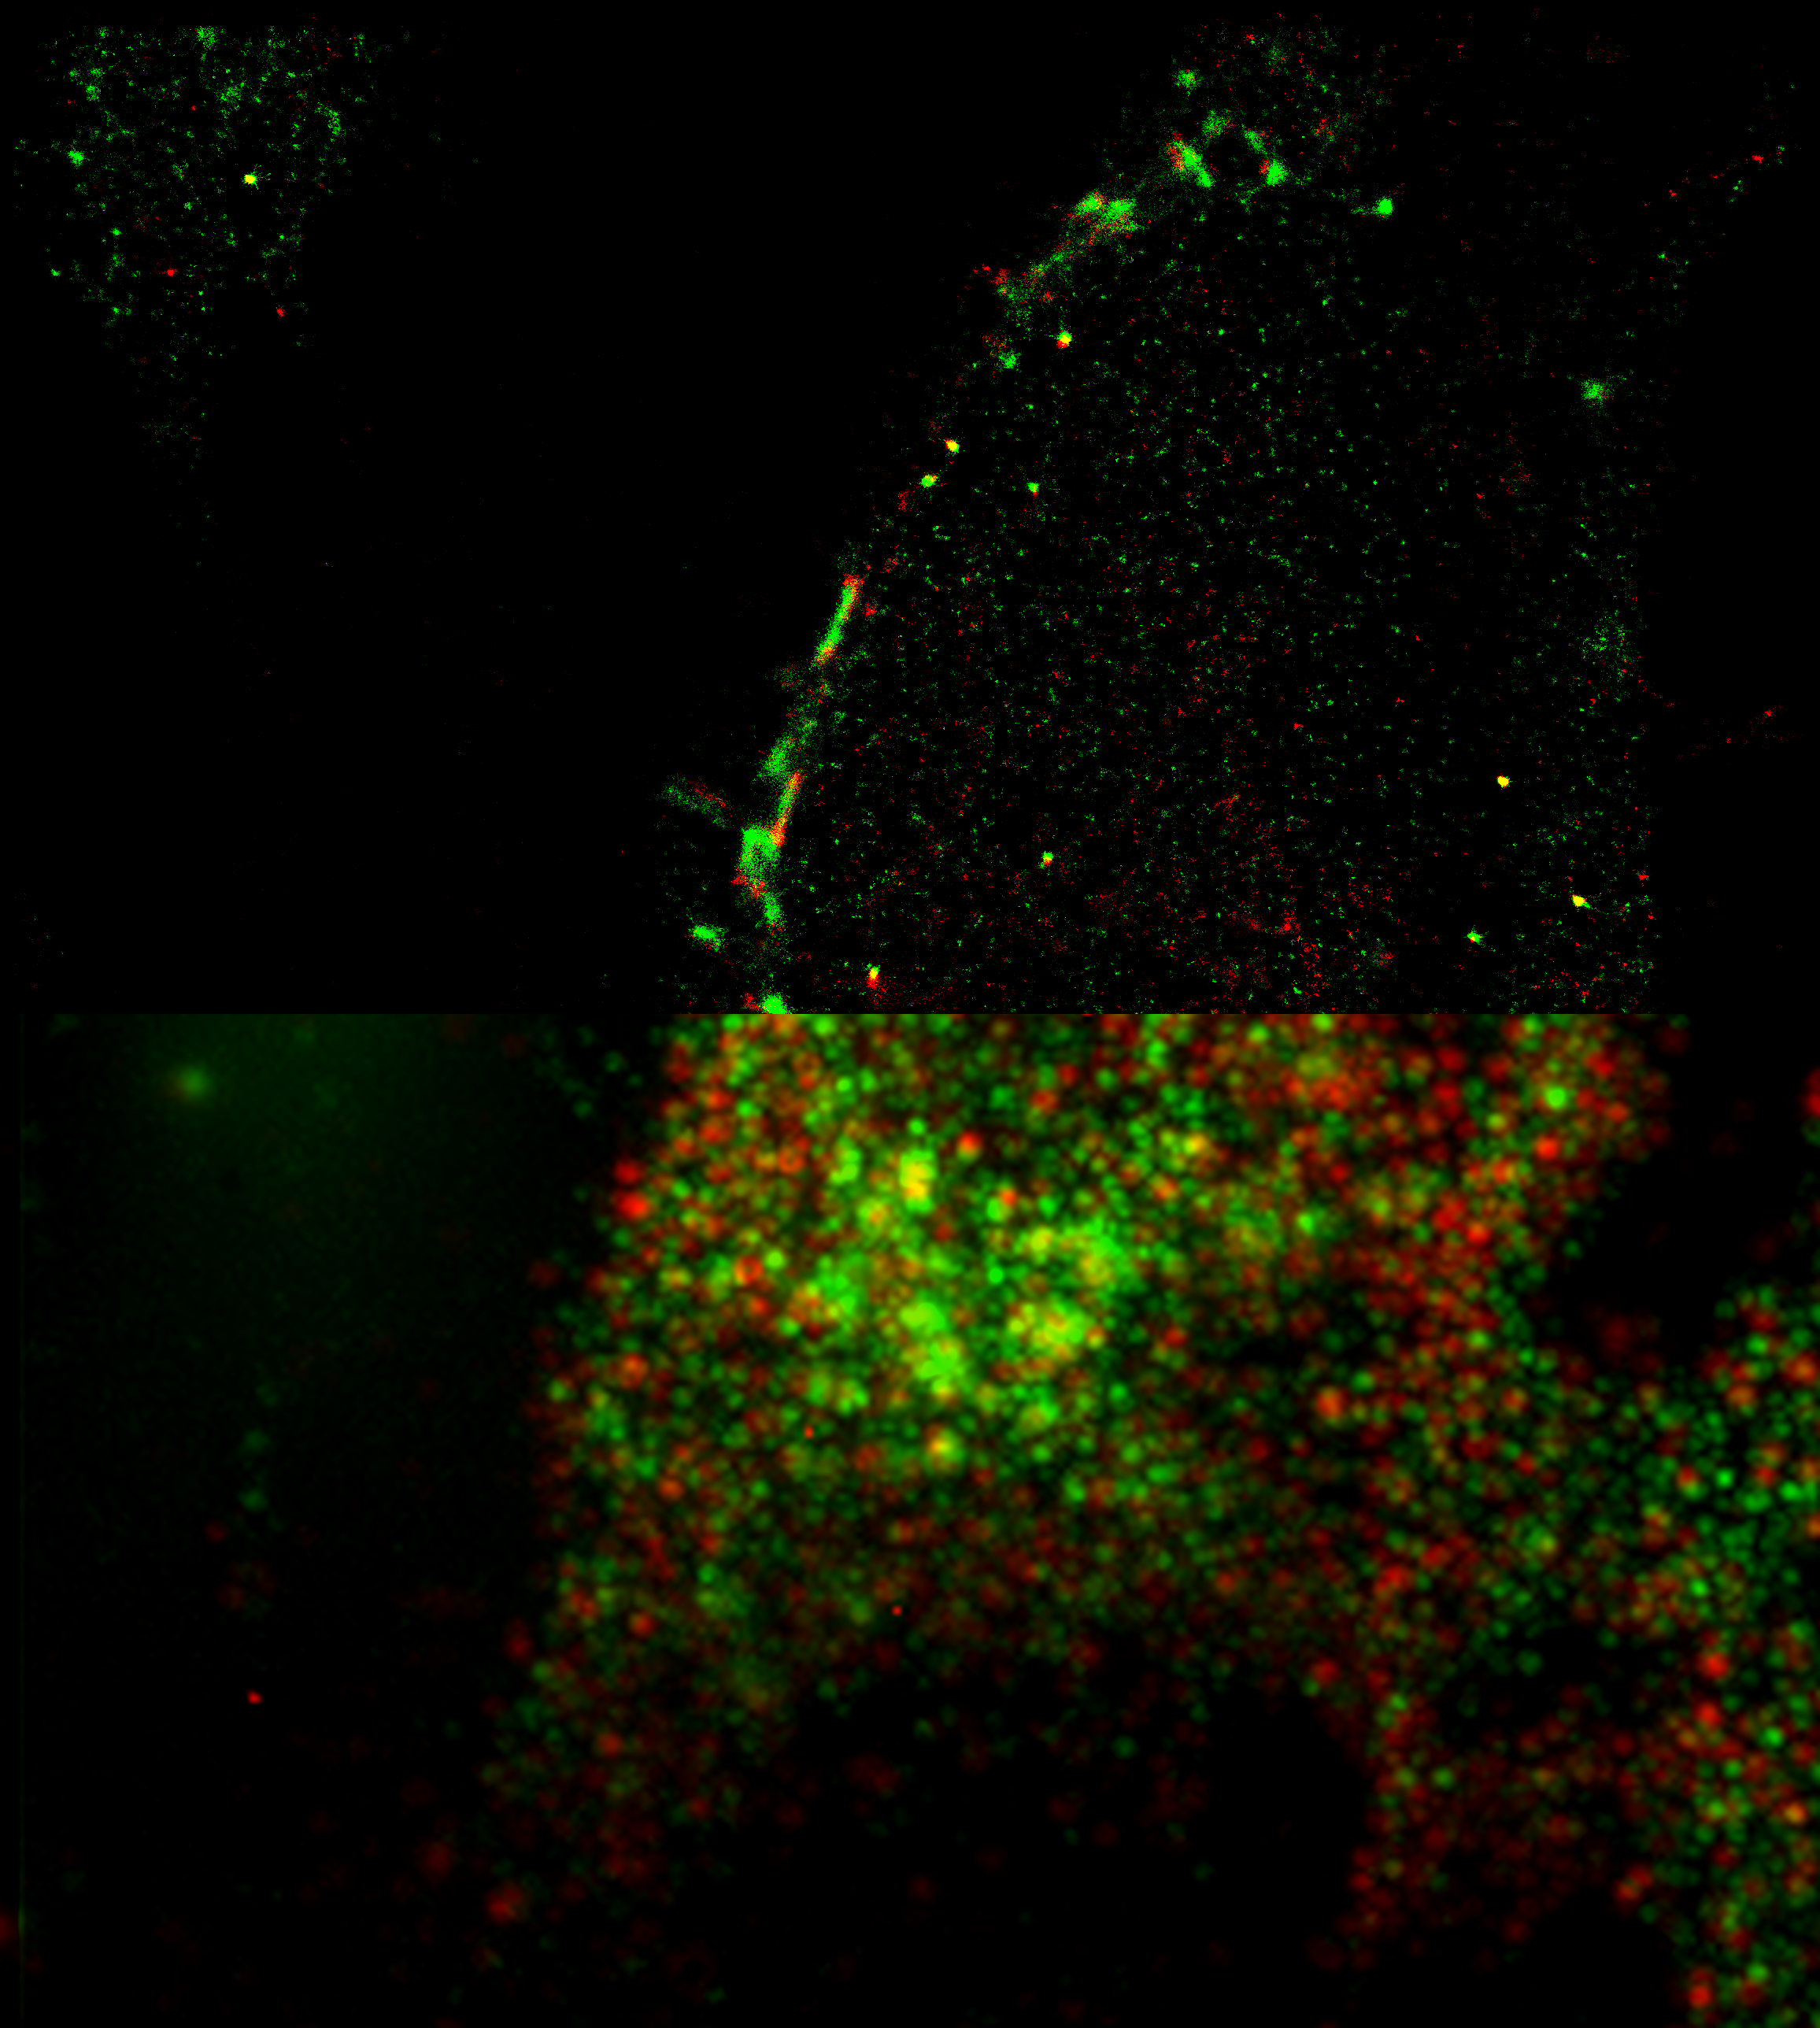
\includegraphics[width = 0.88\textwidth]{pictures/alignedStormWidefield.png}
	\caption{Dual-color image of a cell treated with nocodazole. The upper part shows the reconstructed and aligned image, the lower part the maximum projection of the raw data over all frames.}
	\label{dualcolor}
\end{figure}



\chapter{Theoretical background}
This chapter gives an overview over the most important distributions and transformations that are used for the SimpleSTORM algorithm and the Colorcomposer. An introduction to the most important parts of regular Charge-coupled Device (CCD) cameras is also given, as well as a section about the data the algorithm is designed for. 

\section{The data}
\subsection{Labeling}
The concept of direct stochastic optical reconstruction microscopy (dSTORM) (\cite{heilemann}) is, to label structures of interest with fluorophors that can be exited using a laser with the appropriate wavelength directly, in contrast to STORM techniques which need an additional activator fluorophore. Shortly after the activation the fluorophors emit a photon and fall back to the unexited state or lose the ability to get exited, they bleach out. Special fluorophores have to be used that have a low probability to get activated. Each fluorophore is visible only every thousandth frame or even less frequently. A movie that shows the frames consecutively shows blinking spots.\newline
The technique to stain the samples that was used for all real-world images in this thesis is called immunofluorescence. For this technique antibodies are used to attach the fluorescenic molecules to the samples. Antibodies target specific biomolecules within a cell that show their antigen. There are two classes of immunofluorescence techniques.\newline
Primary immunofluorescence uses only one antibody that the fluorophore is directly attached to.\newline
For secundary immunofluorescence two kinds of antibodies are used. First the primary antibody that binds to the molecule or structure of interest and then a second antibody that binds to the primary and carries the fluorophore.

\subsection{Description of the data sets}
The datasets for dSTORM microscopy that we recieve from our collaborators from
Bioquant, Heidleberg are big datasets of several gigabyte in the Andor ".sif" format. Each
file contains a stack of pictures, usually between 1000 and 10000, taken
consecutively with a fixed exposure time normally between 20 and 200 milliseconds. From now on the first two dimensions are called spatial dimensions. The third dimension of the data, resulting from the consecutive capturing of the images, is refered to as temporal dimension.\newline

Figure \ref{rawStorm} shows a typical frame of raw data. In each frame there might be multiple fluorophores visible at the same time. Due to the large magnification, beyond the diffraction limit, the almost pointlike fluorophores appear as approximatly Gaussian shaped signals, their point spread functions. The fluorophores are either attached to the biological structures that are of interest or form a cluster, called a bead.\newline

Beads are larger and brighter than spots from only one fluorophore and are used to align multiple channels in the postprocessing step. Designed to show up in every frame of the sequence at the same position they can be used as landmarks for alignment. They are composed of fluorophores of different colors to be visible in every channel.\newline

The other spots, such as spots from fluorophores bound structures, often proteins of interest, only light up for a very short time. This is the key aspect of STORM. Instead of one frame that shows all fluorophores at the same time, thousands of frames are captured containing only a couple of point spread functions per frame. This makes it possible to determine the center of each point spread function with a sub-pixel precision. A high resoluion image, with resolutions beyond the diffraction limit, can be reconstructed by plotting all detections found into one image.

\begin{figure}
\centering
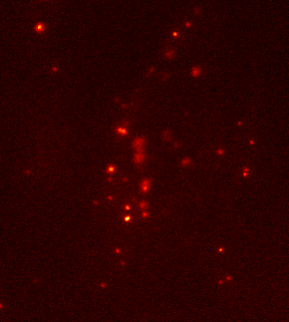
\includegraphics[width = 0.88\textwidth]{pictures/Pos2_2_red2-2frame2475Color.png}
	\caption{Raw image for dSTORM processing}
	\label{rawStorm}
\end{figure}


\section{Distributions}
\subsection{Gaussian distribution}
The Gaussian distribution is characterised by its mean $\mu$ and its variance $\sigma^2$ which is its standard deviation squared. The probability density function is:
\begin{align}
f(x) &= \frac{1}{\sqrt{2\pi}\sigma}\text{exp}\left(-\frac{(x-\mu)^2}{2\sigma^2}\right)&\text{1-D}\\
f(x_1,...,x_k)&=\frac{1}{\sqrt{(2\pi)^k \text{det}(\Sigma)}}\text{exp}\left(-\frac{1}{2}(\bf{x}-\pmb{\mu})^T\Sigma^{-1}(\bf{x}-\pmb{\mu})\right) &\text{$k$-D}
\end{align}
$\Sigma$ is the covariance matrix, $\pmb{\mu}$ is the $k$-dimensional mean. Figure \ref{poisgaussdistr} shows some Gaussian distributions. The two dimensional Gaussian distribution is used for the Gaussian filter.
\subsection{Poisson distribution}
A very important probability distribution in Physics is the Poisson
distribution. Its probability mass function is:
\begin{equation}
	p(n,\mu) = \frac{\mu^n}{n!}\exp(-\mu)
\end{equation}
The larger the mean value $\mu$ becomes the more likely the Poisson distribution results in a Gaussian distribution with a mean and a variance of $\mu$. Figure \ref{poisgaussdistr} shows Poisson and Gaussian distributions with different parameters. The mean value of the gaussian was shifted by 0.5 which results from continuity correction.\newline
Poisson distributions describe the results of ``counting experiments'' and are
therefore important for image processing as pictures taken with a
camera are in principle counts of photons reaching the camera.  \newline
A Poisson distribution is defined for integer values only and its variance is
the same as the mean value of the distribution.\newline
The median of a Poisson distribution is approximatively given by
\begin{align}
	\text{median Pois}(\lambda) \approx \lambda + \frac{1}{3} - \frac{1}{50\lambda} \label{meanMedianPoiss}
\end{align}
Another important attribute is
the skewness which describes the assymetry of the distribution.
\begin{align}
 \text{skewnes Pois}(\lambda) = \frac{1}{\sqrt{\lambda}}
\end{align}
The sum of Poisson-distributed independent variables is also Poisson-distributed.
\begin{figure}
\centering
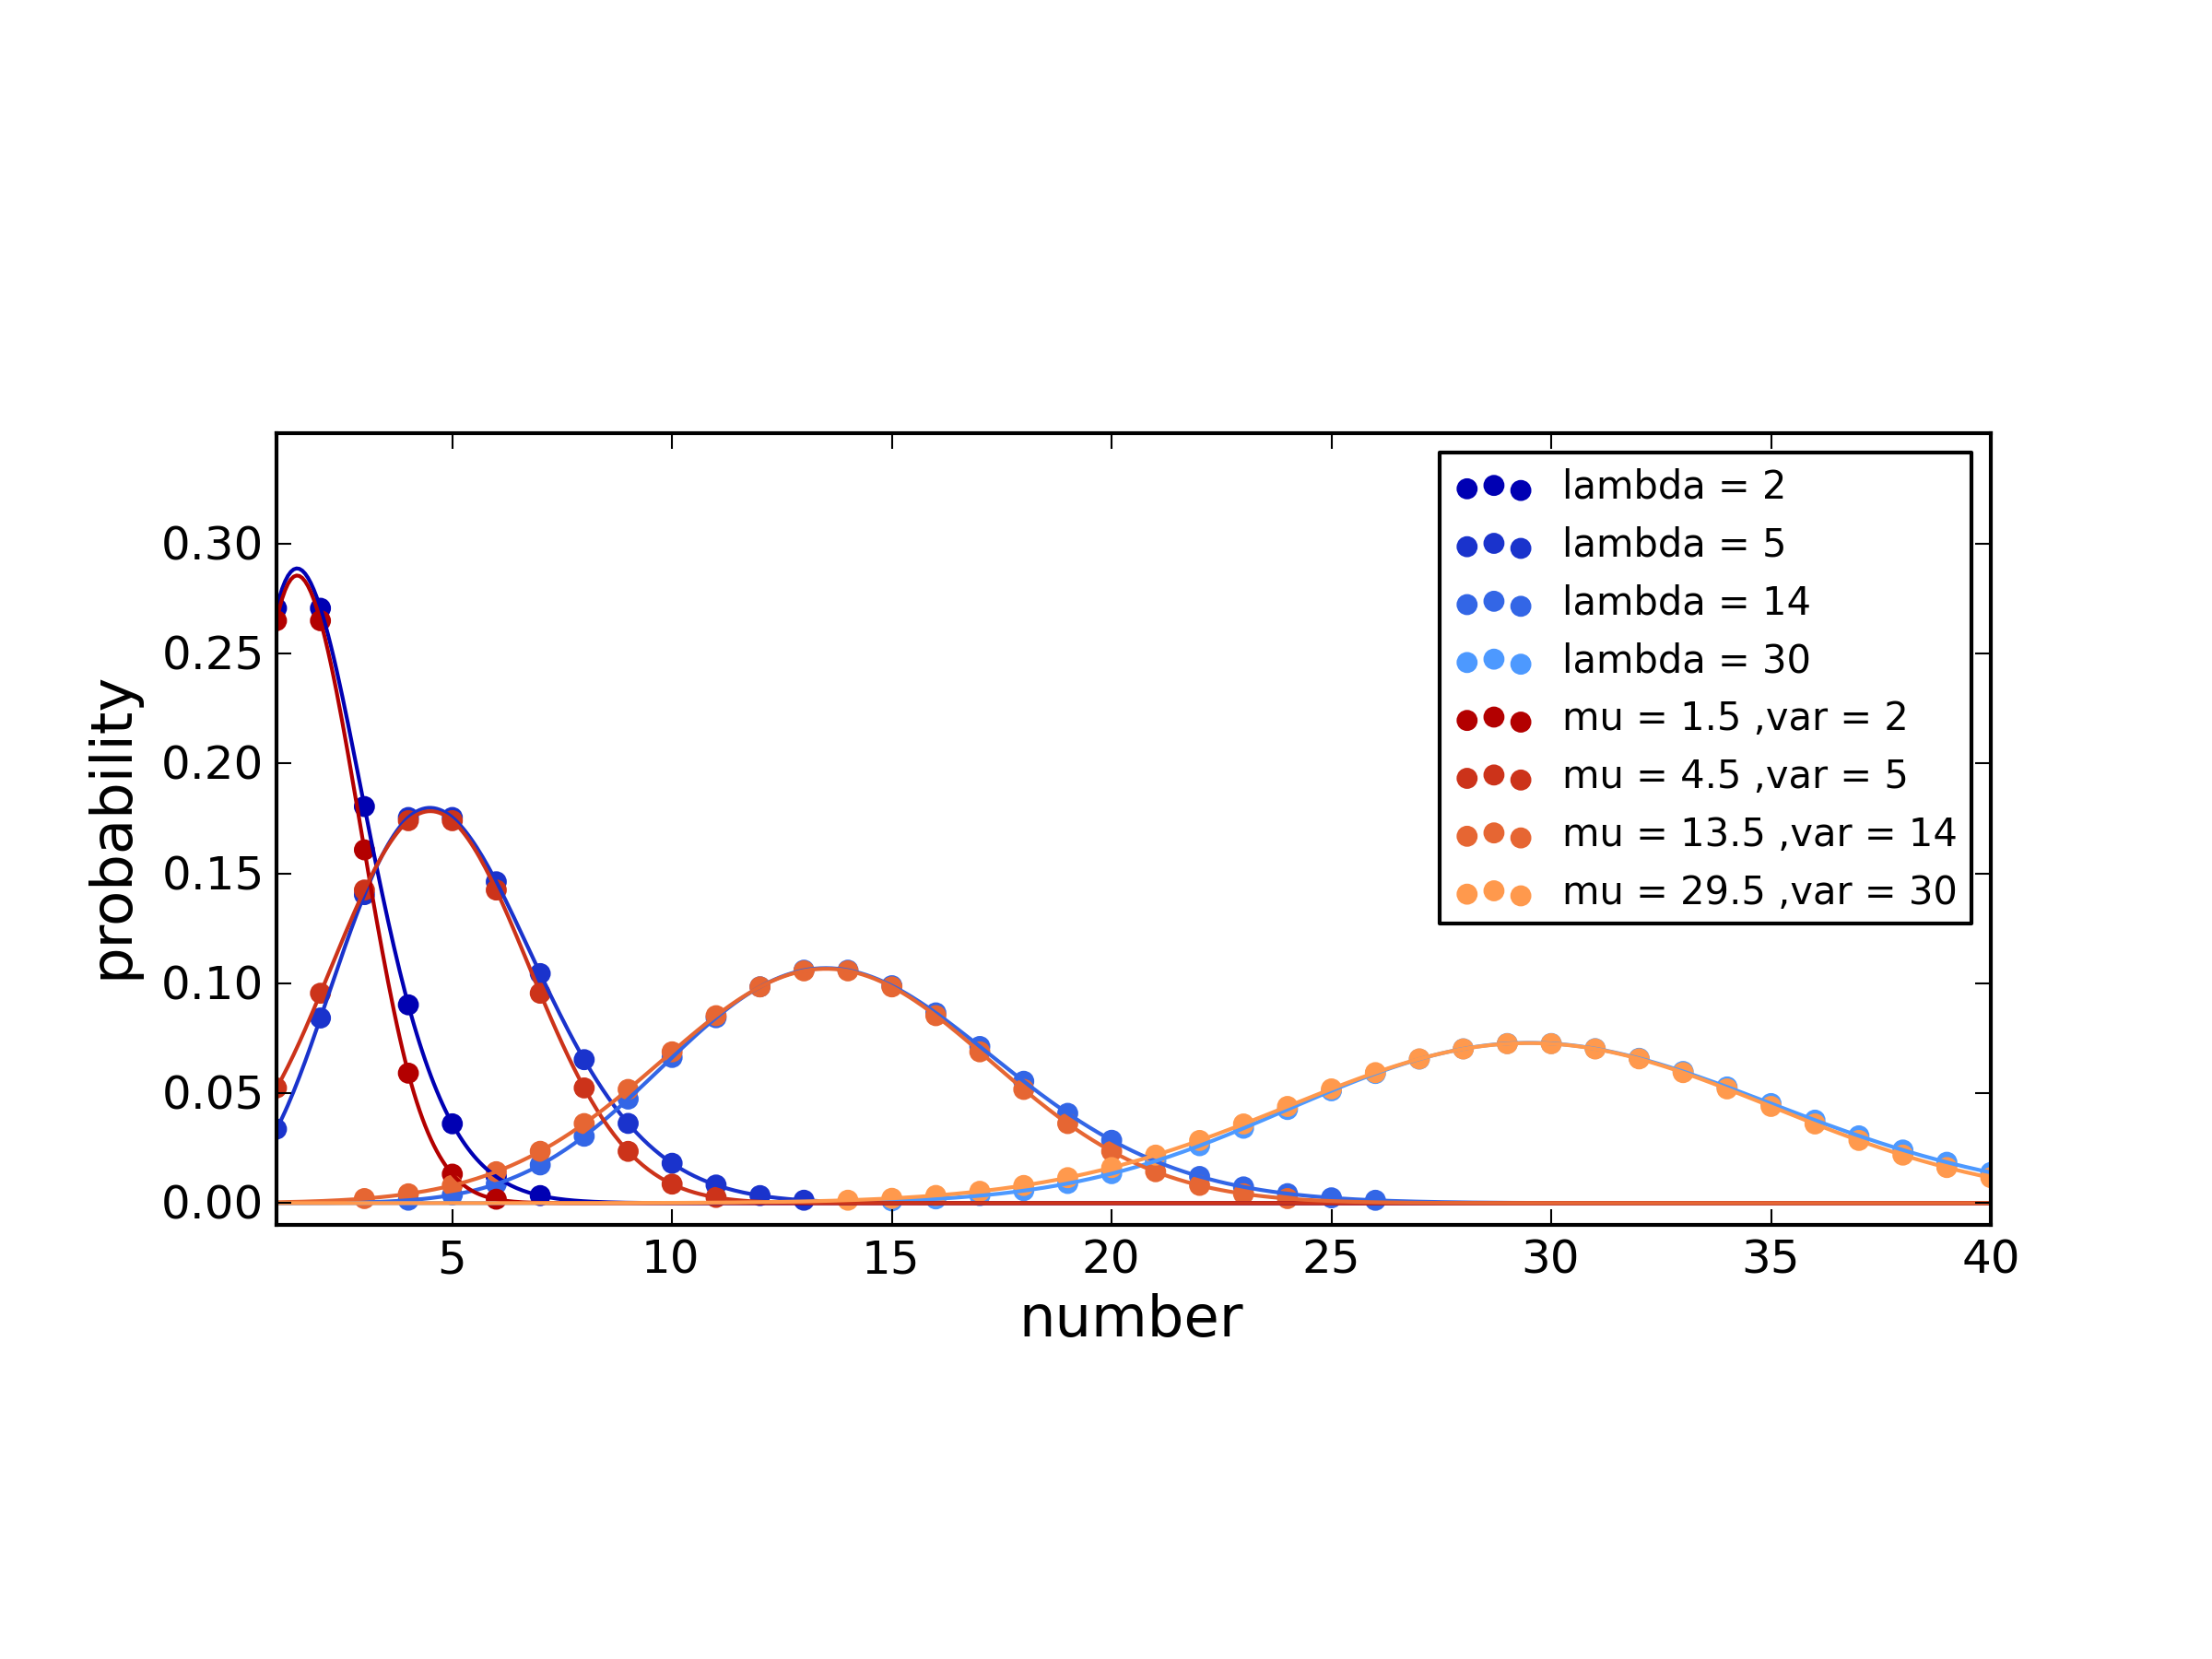
\includegraphics[width = 0.9\textwidth]{pictures/poissgaussdistr.png}
	\caption{Poisson and Gaussian distrubutions with different parameters. Especially for small numbers the Poisson and the Gaussian distribution differ. The larger $\mu$ gets for the Poisson distribution the more similar it gets to a Gaussian with mean $\mu$ and sigma $\sqrt{\mu}$. The Poisson distributions were interpolated between their defined values. For better comparision the integer values of the Gaussian distribution were also marked with dots.}
	\label{poisgaussdistr}
\end{figure}

\subsection{Skellam distribution}\label{skellamdist}
The variance of a Poisson distribution can be estimated using a Skellam distribution based.
The probability
mass function of the Skellam distribution is a function of the difference between
two Poisson random variables
\begin{equation}
	p(k;\mu_1, \mu_2) =
	\exp(-(\mu_1+\mu_2))\left(\frac{\mu_1}{\mu_2}\right)^{k/2}~I_{|k|}\left(2\sqrt{\mu_1
	\mu_2}\right)
\end{equation}  
$n_1$ and $n_2$ are the Poisson distributed random variables and $k = n_1 - n_2$.
$I_{|k|}$ is the modified Bessel function of the first kind.\\
Mean $\mu$ and variance $\sigma^2$ of the Skellam distribution are given by
\begin{align}
	&&\mu &= \mu_1 - \mu_2,& \sigma^2 &= \mu_1 + \mu_2\\
	\Rightarrow &&\mu_1& = \frac{\mu + \sigma^2}{2},& \mu_2 &=\frac{-\mu +
	\sigma^2}{2}
\end{align}
Figure \ref{skellamdistfig} shows two Poisson distributions ($P_\text{red}$ and $P_\text{blue}$) and the resulting Skellam distribution (puple) of the difference $P_\text{blue} - P_\text{red}$.
\begin{figure}
\centering
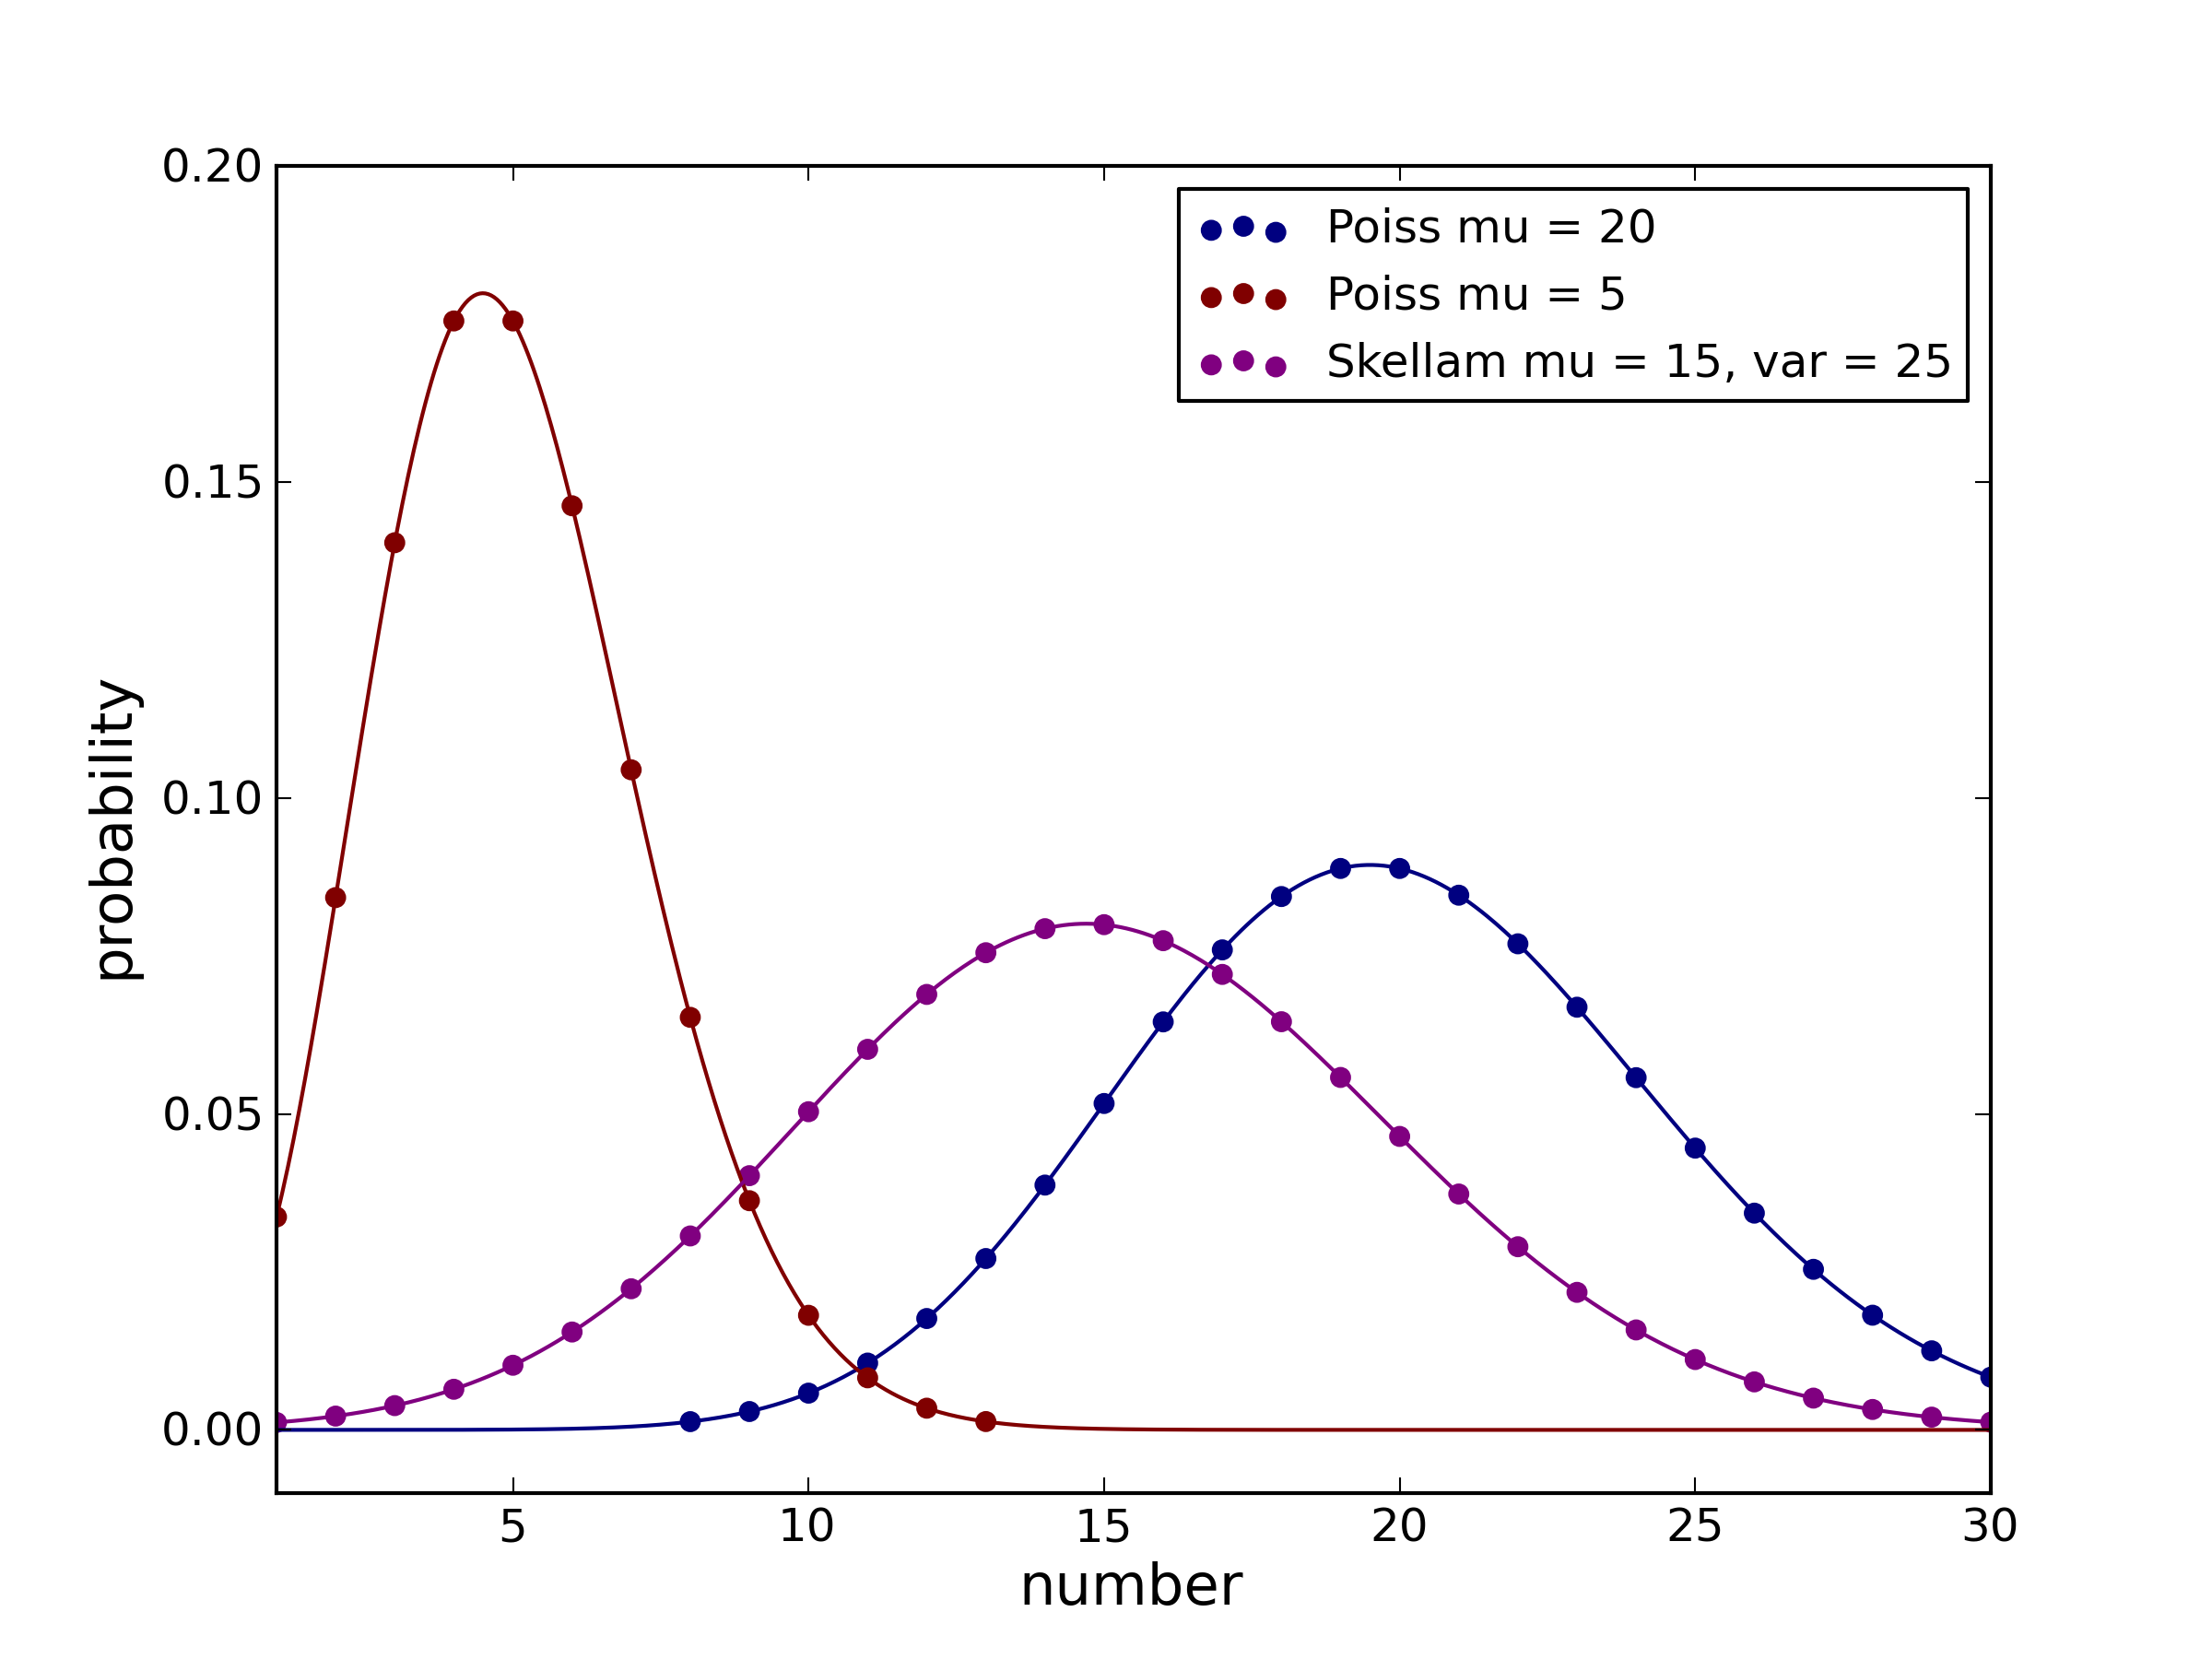
\includegraphics[width = 0.7\textwidth]{pictures/skellamdist.png}
	\caption{Two Poisson distributions and the resulting Skellam distribution. The distributions were interpolated between the integer values.}
	\label{skellamdistfig}
\end{figure}
If the differences between following values of a single Poisson distribution are used for the Skellam distribution the variance of the Poisson distribution is given by the Skellam parameters $\mu_1$ or $\mu_2$ (the mean of the Skellam distribution $\mu$ will be close to zero if the same Poisson distributions are used).\newline
In section \ref{skellambettervariance} is shown which way to estimate the variance works better and more reliable.



\section{Charge-coupled Device (CCD) camera}
The light emmited by the fluorophores is captured by a CCD camera. During the capturing process the true measure, the photons arriving at the aperture of the camera, is transformed to electrons and eventually to a digital number. This section gives a short overview over the most important parts of the signal processing within a CCD camera.
\subsection{Photon counting noise}
The emission of photons is a random process that occures at unpredictible times. Therefore the number of photons passing through a plane is never constant but varies around some average value. This means, that one can never determine exactly how many photons will hit the sensor chip of a CCD camera for example. This phenomena is called shot noise. It playes a major role if the total number of photons is low, for example from dark sources or with short exposure times of the camera.
\subsection{Quantum efficiency}
Quantum efficiency describes the fraction of photons creating a detectable electron in a sensor chip. The quantum efficiency depends on the wavelenght of the incoming photon. Photons with energies below the band gap can not produce a free electron that can be detected. The quantum efficiency has a maximum for a certain wavelength. This maximum of the quantum efficiency is basically caused by two effects. The higher the energy of the photon is the higher is the kinetic energy of the freed electron and therefore the diffusion length is greater, but the electron is absorbed further from the detector and is more likely to recombine with an electron hole.
\subsection{Gain}
There are two different gain factors involved in the capturing process of a camera. Firstly the electric signal for each pixel may be amplified. Secondly there is a gain factor that describes the proportionality between collected electrons and the digital number it is associated with.
\subsection{Readout noise}
The origin of readout noise is the amplifier. The amplification is never perfect, this means that the exact number of electrons at the end of the amplification variates around the expected linearly increased value. There might also be some random signals in the electronics adding to the "true" signal. The readout noise does not depend on the exposure time.
\subsection{Dark current noise}
The dark current noise is generated by the thermal movement of the atoms in the sensor chip. The movement of molecules and atoms depends on the temperature of the material, therefore the dark current noise strongly depends on the temperature of the chip and can be reduced by cooling. Dark current noise generates electrons in the bins of each pixel, even with closed shutter. It increases constantly with time and follows Poisson statistics.
\subsection{Quantisation}
The signal must fit into the output color depth. It has to be rounded or truncated to fit in. This process introduces errors that can be seen as additional noise that is dependent on the intensity of the signal. High intensities are disturbed less relative to low intensies.


\section{Transformations}
\subsection{Transformation to Poisson distributed signal} \label{trafoPoiss}
The images aquired from the camera do not show the real intensities
$I_\text{true}$, which result from the photon emission of the probe, but
transformed ones $I_\text{meas}$.\newline
A linear transformation of the data is assumed with two parameters, the gain $g$ and the offset $o$.
Incoming photons create electrons via inner photoelectric effect. These electrons
are collected for each pixel and might be amplified to get the final result.
Assuming a linear relation between the number of incoming photons and the number
of electrons created and a linear amplifier results in a factor $g$. This factor
is multiplied with the number of photons captured during exposure time for each
pixel.\\
There might also be a constant offset for the pixel intensities that is not affected by the gain factor.
If the gain factor $g$ and the offset $o$ are known the true intensity, the
number of photons detected is:
\begin{equation}
	I_\text{true} = \dfrac{I_\text{meas}-o}{g}. \label{transtopoiss}
\end{equation}
After this transformation the intensities of the background are assumed to be Poisson distributed.
\subsection{Anscombe transformation}
\label{trafoAnscombe}
The Anscombe transform \cite{anscombe} is used to transform a random variable with a Poisson
distribution into one with an approximatly constant standard deviation. The
transformation is defined as:
\begin{equation}
	A(x) = 2\sqrt{x+\frac{3}{8}}
\end{equation}
Figure \ref{anscombe} shows the standard deviation of Poisson distributions with increasing mean (green line) and the standard deviation of Poisson distributions that are transformed unsing the Anscombe transformation (blue line). As can be seen in Figure \ref{anscombe} the Anscombe transformations result has
an intensity independent standard deviation of one for mean intensities greater than 4.
\begin{figure}
	\centering
	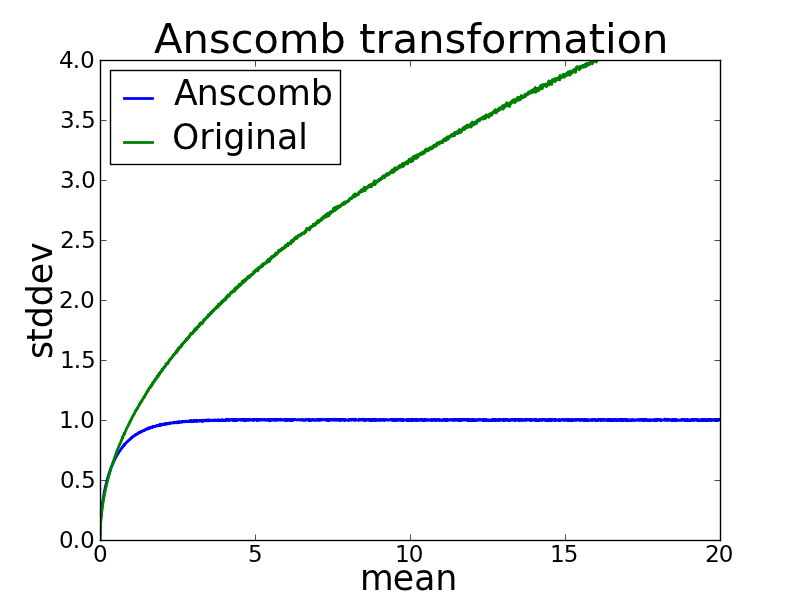
\includegraphics[width = 0.5\textwidth]{pictures/anscombe.png}
	\caption{Standard deviation over mean intensities of different Poisson
	distributions (green) and their Anscombe transformed distributions (blue)}
	\label{anscombe}	
\end{figure}
 

\section{Estimation of camera gain and offset}\label{estimationCameraGain}
Two different ways of estimating the camera parameters have been investigated. For both approaches it is assumed that the background and the beads are Poisson distributed. This data $I_\text{true}$ is then transformed in the following way:
\begin{equation}
	I_\text{meas} = g \cdot I_\text{true} + o \label{trafoGain}
\end{equation}
This is the inverse transformation of equation \ref{transtopoiss}.
\subsection{Using variance-mean plot} \label{skellam1}
The approach for the parameter estimation using the variances of the pixels is shown using a minimalistic example. It is then used in a generalised form.\newline
Consider two pixels with different Poisson distributions $P_1$ and $P_2$ with mean value and variances of this distributions $\lambda_1$ and $\lambda_2$. If these distributions are transfomed as given in equation \ref{trafoGain} their mean and variance in temporal domain change as shown in equation \ref{meanvarPoiss1} and \ref{meanvarPoiss2}. This allows to determine the gain and offset using only two pixels.
\begin{align}
	\text{var}(I_{\text{meas}1})& = g^2\cdot\text{var}(I_{\text{true}1}) \label{calcvar}\\ 
	\text{var}(I_{\text{meas}2})& = g^2\cdot\text{var}(I_{\text{true}2})\\
	\text{mean}(I_{\text{meas}1})& = g\cdot \text{mean}(I_{\text{true}1}) + o\\
	\text{mean}(I_{\text{meas}2})& = g\cdot \text{mean}(I_{\text{true}2}) + o
\end{align}
The values for $\text{var}(I_{\text{meas}1}), \text{var}(I_{\text{meas}2})$, $\text{mean}(I_{\text{true}1})$ and $\text{mean}(I_{\text{true}2})$ can be calculated from the data and can be used to calculate the gain as follows:
\begin{align}
	\frac{\text{var}(I_{\text{meas}1})-\text{var}(I_{\text{meas}2})}{\text{mean}({\text{meas}1})-\text{mean}(I_{\text{meas}2})}&= \frac{g^2\cdot \lambda_1  - g^2\cdot \lambda_2 }{g\cdot \lambda_1 + o - (g\cdot \lambda_2+o)}\\
	& = \frac{g^2\cdot(\lambda_1-\lambda_2)}{g\cdot (\lambda_1-\lambda_2)}\\
	& = g
\end{align}
The offset $o$ can be calculated in the same way.
\begin{align}
	\text{mean}(I_{\text{meas}1}) - \frac{\text{var}(I_{\text{meas}1})}{g} &= g\cdot \lambda_1 + o - \frac{g^2\cdot\lambda_1}{g}\\
	&= o
\end{align}
The estimation gets more stable if more than two points are used and if the points are taken from a wide range of intensities. If more than two points are used a straight line must be fitted through them. This lines slope gives the gain factor and the intersection on the $x$-axis the offset. The variance of the pixels intensities are calculated directly, instead of using the Skellam approach. This is motivated in section \ref{skellambettervariance}.
\subsection{Using skewness of poisson distribution}
A second approach is to use the skewness of the Poisson distribution to estimate the mean value.\newline
For every pixel there are multiple intensities in temporal dimension. One can
calculate mean and variance of the measured intensities for each pixel $I_\text{meas}(i,j)$ and
gets
\begin{align}
	\text{mean}(I_\text{meas}(i,j))& = g\cdot \text{mean}(I_\text{true}(i,j)) + o \label{meanvarPoiss1}\\
	\text{var}(I_\text{meas}(i,j))& = g^2\cdot\text{var}(I_\text{true}(i,j)) \label{meanvarPoiss2}
\end{align}
Assuming a Poisson distribution as the true intensity, mean and variance would
be the same. Unfortunately the mean true intensities are unknown and it is
not possible to determin $g$ and $o$ so far. For large mean Intensities $\mu$
the Poisson distribution becomes more and more symmetric and therefore similar to a Gaussian distribution
with the same mean and variance as the Poisson distribution. However, for small means, the Poisson distribution is not
symmetric. The skewness $s_p$ of a Poission distribution is the inverse of the
square root of the mean $(\mu)^{-.5}$. It can also be directly
calculated from data
\begin{equation}
	s_p = \frac{1}{n}\sum_{i = 1}^n \left(\frac{x_i - \bar x}{\sigma}\right)^3
\end{equation}
The skewness is invariant to shift and multiplication with a constant. This
means that the transformation caused by the camera gain and the offset
does not affect the skewness. This gives a third equation to solve for $g$ and
$o$.\\
This approach is strictly limited to, at least for background pixels, low intensities. Tests have shown that if the mean of the true Poisson distribution is higher than roughly 30, the skewness gives no stabel results. This is shown in section \ref{skewnesssucks}. For data sets with high background intensities it is not possible to determine the camera parameters in this way.

\section{Check for correct gain factor} \label{checkGain}
The gain factor may have been determined or entered incorrectly. Assuming there is the true gain factor $g_\text{true}$ and the incorrect gain factor $g_\text{false}$. Let be Poiss$(\mu)$ the true Poisson distribution of one background pixel and $o$ the offset. The pixels raw intensities are therefore $g_\text{true} \cdot \text{Poiss($\mu$)} + o$. The following shows the effects of the incorrectly chosen gain factor on the transformed images:
\begin{align}
	\frac{(g_\text{true} \cdot \text{Poiss($\mu$)} + o)-o}{g_\text{false}} &= \underbrace{\frac{g_\text{true}}{g_\text{false}}}_{r}\text{Poiss($\mu$)}&\text{Transformation \ref{trafoPoiss}}\\
	2\sqrt{r\text{Poiss($\mu$)}+\frac{3}{8}}&\approx \text{Gauss}(2\sqrt{r\mu},r)&\text{Transformation \ref{trafoAnscombe}}
\end{align}
The variance of the Gaussian can be determined. Since the incorrect estimate of the gain factor and the Gaussians variance $r$ are known, the correct gain factor can be determined by multiplication of the incorrect one with $r$.

\section{Filters}
\subsection*{Gaussian filter}
The Gaussian filter uses a Gaussian for the convolution with the image that shall be filtered. The convolution of an image with a Gaussian filter alters the intensities of the pixels by adding some fraction, depending on the parameters of the filter, of the intensities of the surrounding pixels. The Gaussian filter can be used for noise suppression.
\subsection*{Wiener filter}
The Wiener filter is also known as Wiener-Kolmogoroff filter. One application of the Wiener filter is noise suppression. It is designed to minimize the mean square error of the filtered image compared to the original image without noise. 
%\chapter{CCD camera}

\section{Image acquisition}
\subsection{Photon sources with shot noise}
The emission of photons is a random process that occures at unpredictible times. Therefore the number of photons passing through a plane is never constant but varies around some average value. The phenomena, that one can never determine exactly how many photons should hit the sensor chip of a CCD camera for example, is called shot noise. It playes a major role if the total number of photons is low, as from dark sources or with short exposure times of the camera.
\subsection{Quantum efficiency}
Quantum efficiency describes the fraction of photons that create a detectable electron in a sensor chip. The quantum efficiency is dependent of the wavelenght of the incoming photon. Photons with energies below the band gap can't produce a free electron that can be detected. The quantum efficiency has a maximum basically caused by two effects. The higher the photons energy the higher the kinetic energy of the freed electron, but it is absorbed earlier and can therefore recombinate with a electron hole more likely.
\subsection{Gain}
There are two different gain factors involved in the capturing process of a camera. First the electric signal for each pixel might be amplified. And there is also a gain factor that describes the proportionality between collected electrons and the digital number it is associated with.
\subsection{Readout noise}
The origin of readout noise is the amplifier. The aplification is never perfect, this means the exact number of electrons at the end of the amplification has some variation around the expected linearly increased value. There might also be some random signals of the electronics that add to the "true" signal. The readout noise is independent of the exposure time.
\subsection{Dark current noise}
Dark current noise is generated by the thermal movement of the atoms in the sensor chip. The movement of molecules and atoms is dependent of the temperature of the material, because of that dark current noise depends strongly on the temperature of the chip and can be reduced by cooling. Dark current noise generates electrons in the bins of each pixel even with closed shutter it is constantly increasing with time and follows Poisson statistics.
\subsection{Quantisation}
The signal must fit into the output color depth. It has to be rounded or truncated to fit in. This process introduces errors that can be seen as additional noise that is dependent on the intensity of the signal. High intensities are disturbed less relative to low intensies.

\chapter{The improved SimpleSTORM algorithm}
STORM data from different cells or structures show many different features: there can be clusters of fluorophores with a high density of spots, areas with low density, variable background in space and time, beads can be present or absent.\newline
This section describes how the algorithm processes the data sets and how it is possible to find good settings that will work for all kind of input data. The changes and improvements over the previous version are described and discussed. The new GUI design and the new features are introduced.\newline
All real world images shown in this thesis were acquired from members of Prof. Dr. Mike Heilemanns group.


\section*{Import and processing}
STORM data usually has a size of around 3 gigabytes. However larger data sets are possible too, making it necessary to work on smaller parts of the data, instead putting the whole dataset into memory. This is done using chunks of a user defined size. The data is processed chunkwise, and the processing of the frames of each chunk can be parallelized. This parallelization is possible because the signals in each frame are considered to be independent from each other. There is a dependency between different chunks. The mean values of several chunks are used to estimate the background. Therefore a certain number of mean values has to be stored in memory.

\section{Workflow}
\subsection{Choosing parameters}
Initially the user has the option to set all important parameters. If no parameter is set the default ones are used and will give a good result because all crucial parameters are either determined from the data or set to reasonable values that work for every data set. The goal of the default parameters is to give a good result with no adjustment. This means parameters are chosen to produce almost 100 \% precision. It is assumed that the loss of some points that are not detected using this conservative setting will not affect the final result as much as a lower precision would.
\subsection{Estimating camera gain and offset}
First the application checks for a file containing settings for gain and offset from an earlier run. If this is not the case new parameters are estimated based on the first part of the data; usually 200 frames are sufficient.\newline
A set of 2000 pixels is chosen by their mean intensity with respect to time. Therefore the mean intensity range is divided in 2000 bins. For each bin one pixel with the appropriate mean is selected. For faster computation the mean is not calculated over all frames but only over a certain, user defined, number. The goal is to get pixels with the whole range of mean intensities, good representatives from the darkest background pixel to the brightest beads.\newline 
The method described in section \ref{skellam1} is used to estimate the gain factor, based on the preselected points. The variances of the pixels are computed based on the first part of the data.
Each dataset is three-dimensional, where time is the third
dimension. Therefore mean $\mu$ and variance $\sigma^2$, in time, can be calculated from
the data for each pixel individually
\begin{align}
	\mu(i,j) & = \frac{\Sigma_t(I_t(i,j)(i,j))}{n}\\
	\sigma^2 & = \frac{\Sigma_t(\mu(i,j)-(I_t(i,j)))^2}{n-1}
\end{align} 
$I_t(i,j)$ describes the intensity of the pixel of frame $t$ at position $i,j$.
To determine the gain factor the variances $\sigma^2$ for each pixel are plotted over the mean
intensities. A straight line can be fitted, and its slope gives the gain
factor, the $x$-intersection gives the offset.\newline 
Figure \ref{skellamplot} shows the scatter plot for the selected points and the fitted line. The data is taken from a real world data set. The red dots result from pixels that have a constant mean intensity over time. They are either dark the whole time, these are the dots on the left or they are beads and show signal in every frame. The blue dots result from pixels that are sometimes covered by a PSF. This blinking has much stronger influence on the variance than for the pixels mean values. This is the reason why this points are clustered on the lower end of the mean intensities. \newline
For a robust estimation of the straight line a RANSAC (random sample consensus) algorithm is used. It is described in section \ref{ransacdescr}. 

\begin{figure}
\centering
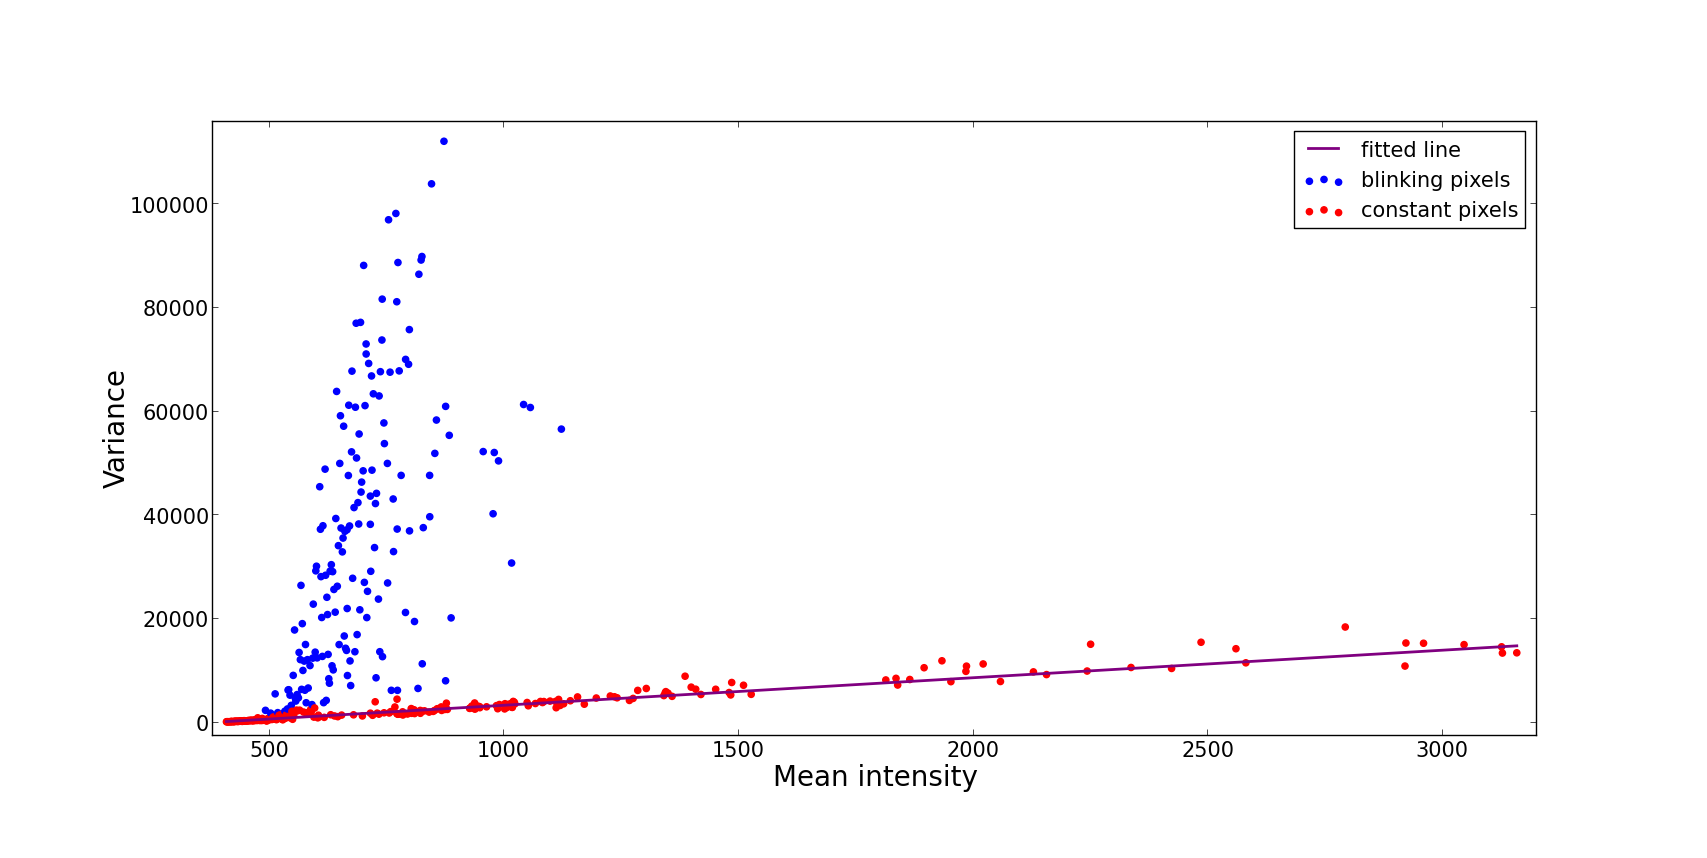
\includegraphics[width = 0.99\textwidth]{pictures/skellamplot.png}
	\caption{Scatter plot for the preselected points. Blue points result from pixels that show at least once a higher intensity caused by a fluorophore. The red dots are used to determine the gain and offset.}
	\label{skellamplot}
\end{figure}
\subsection{Recursively adjusting gain and offset}
After the estimation of gain factor and offset, the transformations described in section \ref{trafoPoiss} and section \ref{trafoAnscombe} are applied and the background is subtracted.\newline
Due to the Anscombe transformation, the background pixels of the image should only vary around a mean intensity of zero with a variance of one. Therefore, a histogram of the pixel intensities is created. After background subtraction, the background pixels should contribute only to the lower intensities in the histogram. A Gaussian function is fitted to the histogram's values. This is done under the assumptions that there is much more background in the image than signal, or that the intensities coming from signals are distributed over a larger range, so the Gaussian for the background intensity distribution can be fitted correctly.\newline


If the estimated value for the variance is too far from one, the originally estimated gain factor is corrected and applied, and the fit is done again (compare section \ref{checkGain}). This is done until the background variance converges within a small threshold or the maximal number of iterations is reached. In this case the initial gain factor will be used and a warning will be shown on the screen.\newline
It might be that the correction of the gain factor gets trapped duo to overshooting. In that case the estimated background variances oscillate around one. If this is the case the mean gain factor from the last two corrections is used.
\subsection{Estimating the width of the point spread function}
An inverse Anscombe transformation (equation \ref{invAnsc}) is applied to the data. This is necessary because the Anscombe transformation increases the point spread functions width, depending on the intensity of the point spread function. This is shown in section \ref{PSF}.\newline  
For 20 local maxima of a certain, user defined, number of frames the square of the Fourier transformation off each region of interest around the chosen local maxima is calculated. This squared Fourier transformations are then averaged. The result is called the mean power spectrum. It can be used to estimate the variance of the point spread function of the signal. A two dimensional Gaussian function's Fourier transform is again a Gaussian but with inverse variance. This relation is used to determine the variance of the point spread function in the spatial domain, using the fit parameter for the variance in the frequency domain.\newline
The script for fitting the two dimensional Gaussian function was implemented by Ilia Kats.
\subsection{Processing the data}
\subsubsection{Import Data}
Storm data sets can consist of several thousand frames with resolutions up to one megapixel per frame. This size makes it necessary to break the data into smaller parts, otherwise it could be larger than the RAM of an ordinary machine. Because of the background estimation, it is not possible to process every frame completely independently as it was in the older version of this software (\cite{MAJoachim}). 
%For the hdf5 data format it is faster to load a larger consecutive part of the dataset into memory instead of loading each frame.
\newline
This algorithm uses chunks of user defined size. There are some limitations to the chunk size that are discussed later. The data set is split into parts of equal size in the $x$- and $y$-dimensions and independently also in the $t$-dimension. If this partition does not fit at the edge of the data set, the last chunks will be smaller.\newline
The data is transformed to be Poisson distributed, then the Anscombe transform is applied which gives background intensities with unit variance.\newline
The implementation of the workflow using chunks was done by Ilia Kats.
\subsubsection{Background estimation} \label{bgestimation}
For each chunk, the median of the Anscombe transformed data is determined to get a robust estimate of the background value for this chunk. 
B-spline interpolation, implemented in vigra (\cite{vigra}), is used to get interpolated values for the full resolution of the current frames. For this interpolation, three chunks in both the spatial and the temporal domain have to be available. Therefore the maximal chunk size into $t$-dimension must not be larger than a third of the total stack size, the same holds for the chunk size in $x$ and $y$ direction which must not exceed the spatial resolution of the image stack. These values are checked automatically and changed if necessary.\newline
The interpolated background is then subtracted from the transformed data to give background pixels with zero mean and unit variance, both in $xy$- and in $t$-dimension. Figure \ref{removedBG} shows an frame with variable background before and after background subtraction.
\begin{figure}
\subfloat[Original image]{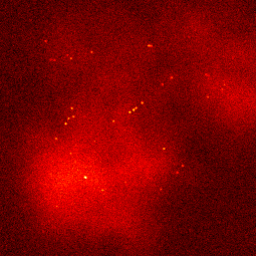
\includegraphics[width = 0.485\textwidth]{pictures/Tubulin2OrigFrame50Color.png}}\hfill
\subfloat[image after background subtraction]{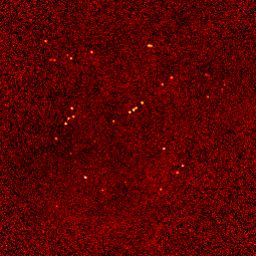
\includegraphics[width = 0.485\textwidth]{pictures/Tubulin2normalprocessFrame50Color.png}}
	\caption{Effect of background subtraction on an inhomogeneous background. For the human eye no more points are visible but for computers it is much easier to find the bright spots in the background subtracted image, because a global threshold can be applied or as in the case of SimpleSTORM the probabilistic model can be tested.}
	\label{removedBG}	
\end{figure}
\subsubsection{Create mask for background suppression}
With the given $p$-value from the settings, a global threshold can be determined, because inhomogeneities of background intensities have been removed. The threshold value is that intensity 
for which the integral over the probability density function of a Gaussian distribution with zero mean and unit variance gives $1-p$. It is that intensity for which it is less likely than $p$ to occur. This threshold is possible because the background intensities follow a Gaussian distribution, with known mean and variance, after all transformations applied.\newline
The threshold is applied to the current frame and a binary mask is stored. For the reason that it is possible for bright background pixels to exceed the threshold, the connected components of the mask are calculated. Pixels that belong to connected components with too few members are discarded. The idea behind using connected components is, that there is a probability for a background pixel to be brighter than the threshold, but it is unlikely that two neighboring pixels exceed the threshold in the same frame and even more unlikely that three of them do so. Therefore the number of pixels necessary for keeping a connected component is set to a minimum of three. If the width of the point spread function is very large the critical size of the connected components can be set depending on the PSF width. But to suppress background pixels efficiently the number of pixels in a connected component has to be larger than two.
\subsubsection{Filtering data and finding maxima}
To improve the accuracy of the spot detection, the transformed signal is convolved with a two dimensional Gaussian function with the previously determined or user-set width. The convolved image will further be used to find the maxima. All local maxima in the frame are detected. Each maximum found is tested to be covered by the mask or discarded otherwise. A region of interest around the remaining maxima is interpolated to a higher resolution. The interpolated region is searched for local maxima once again. These maxima will be detected with super resolution.\\
To determine the signal-to-noise ratio, the unfiltered and uninterpolated pixel intensity is used.
This maxima detection was already implemented by Joachim Schleicher (\cite{MAJoachim}).
\subsubsection{Quality control for detections}
Sometimes, especially in data sets with a high density of spots, two spots are near enough that their point spread functions overlap. It may happen that instead of two maxima only one maximum will be detected between the true ones, as can be seen in Figure \ref{betterthansimplestorm}. This leads to large errors in the localization. To avoid this a threshold for the asymmetry of the spots can be set.\newline
The calculation of the asymmetry was already implemented by Joachim Schleicher \cite{MAJoachim}.


\section{Comparison with older version of the SimpleStorm algorithm}
\subsection{Adjustable filter width} \label{sectionFilterisEvil}
If two or more point spread functions (PSF) overlap, applying a smoothing filter can lead to the merging of point spread functions. This merging becomes a problem if the two distinct maxima of the original unsmoothed PSFs form a new maxima in between. This leads to just one detection somewhere between the true maxima. The number of merging PSFs increases with greater filter widths. For high density data it might be better to use a filter with smaller width and therefore less accuracy, but fewer merged PSFs. In total this might give a better result depending on the number of incorrectly merged PSFs. This is the reason why filtering was changed to use just a Gaussian filter instead of the Wiener filter originally used. 
The effect of the smaller filter width can be seen in Figure \ref{betterthansimplestorm}. The red crosses indicate detections found by the new SimpleSTORM version, the green crosses show the estimated positions found by the previous version of SimpleSTORM, and the white x marks the true location. The predictions by the newer version are not perfect but better than the predictions of the older version. The scores that can be seen in Table \ref{tabelbetterthansimplestorm} are calculated like as described in section \ref{measuresISBI}. Both results have almost the same accuracy, but differ in the scores. There are two effects related to the accuracy canceling each other out. Fewer merged PSFs increase the accuracy, but the positive effect of filtering with the appropriate filter, as shown in Figure \ref{accplot2} or in Figure \ref{matchedFilter1}, is lost.

\begin{table}
\caption{Comparison of results created using almost no smoothing or Wiener filter on high density data. Although the accuracy is almost the same, the number of detections and the scores are higher for the unsmoothed data. For the evaluation software from the \cite{challenge} were used.}
\begin{tabular}{l|llllll}
&intersections&Jaccard&F-Score&Precision&Recall&RMSE\\ \hline
Gaussian filter, $\sigma$ = 0.01& 16955&19.99&33.26&81.10&20.92&27.21\\
Wiener filter& 14480&17.06&29.15&79.19&17.87&27.28
\end{tabular} \label{tabelbetterthansimplestorm}

\end{table}


\begin{figure}
\subfloat[Advanced setting widget]{
\includegraphics[width = 0.485\textwidth]{pictures/betterthanSimplestorm1.png}}\hfill
\subfloat[Easy setting widget]{
\includegraphics[width = 0.485\textwidth]{pictures/betterthanSimplestorm2.png}}
	\caption{This pictures show the effect of a smaller filter width. The red crosses show detections found with a filter width of 0.01, the green crosses the results using a Wiener filter. The white x marks the ground truth.}
	\label{betterthansimplestorm}	
\end{figure}

\subsection{False positive suppression}
In the previous version the background was determined by first estimating a baseline. The minimum of the current frame was taken as the baseline. It was subtracted from the image and the result was smoothed with a Gaussian filter of width ten. The smoothed image was subtracted from the original image to give a background free image. This works fine for subtracting background with variations larger than the filters width, but the resulting intensities do not contain any information about the variability of the background intensities.\newline
If, for example, the resulting intensity, after background subtraction, is five. This can either mean it is most likely signal, given that the variance of the background in the original image was very small, or it can mean nothing, if the variance of the original background pixels were 20. In the latter case the probability that the difference of five between the original image and the smoothed one has a high chance to result from the background variation.\newline
In the older version of SimpleSTORM the intensity of a candidate, considered to be a signal, was checked 
whether its intensity after the background subtraction was higher than the estimated background value at the maximums position minus the baseline. This works for homogeneous background intensities but fails if the baseline, gets a small value from a region with small background values and is applied to a bright region. In that case the intensity of the estimated background gives high values at the maximums position but only a small value is subtracted. This results in discarding many maxima in regions of bright background as in Figure \ref{bgmakesitbad}.
The old version of SimpleSTORM only finds about 8000 spots while the new version finds more than 44000 on a test data set with high background variance. Using the new background suppression results in a reconstructed image that shows the reconstructed structures in a better way.

\begin{figure}
\subfloat[Typical frame showing variable background intensities]{
\includegraphics[width = 0.3\textwidth]{pictures/Tubulin2OrigFrame50.png}}\hfill
\subfloat[Result old SimpleSTORM]{
\includegraphics[width = 0.30\textwidth]{pictures/Tubulin2factor1OldSimpleSTORM.png}}\hfill	
\subfloat[Result new SimpleSTORM]{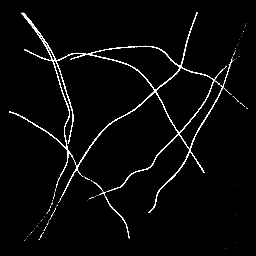
\includegraphics[width = 0.3\textwidth]{pictures/Tubulin2factor1.png}}

\caption{This pictures show the drawback of the old background treatment. On the left a typical frame with variable background is shown. The old version of SimpleSTORM discards many detections in the regions of high background intensity. The new SimpleSTORM software discards detections based on their signal-to-noise ratio and is less affected by variable background.}
\label{bgmakesitbad}	

\end{figure}

The great advantage of the newer version of SimpleStorm is its model for the background. For each pixel, the probability to be signal can be determined based on its signal-to-noise ratio. Using the number of connected components of each cluster, false positive detections caused by bright background pixels can be suppressed.

\subsection{Comparable results based on the signal-to-noise ratio}
The accuracy of the maxima detection relies on the signal-to-noise ratio (SNR). With a given SNR the correct standard deviation of the localization error can be used for further calculations (the calculation for the localization error is done in section \ref{detectionError}). This is not possible if only intensities are saved because without information about the backgrounds variance the reliability of the detection can't be estimated.\newline
Saving the signal-to-noise ratio also enables to compare results from either different cameras or different settings or a different environment that might lead to a higher background variability.  


\section{New graphical user interface (GUI)}
\subsection{Input widget}
The new GUI for SimpleStorm was designed to integrate its many new features. Figure \ref{guiWidgets} shows this new design. \newline
There are three categories of parameters. The first category specifies which upsampling factor will be used, the width of the pixels in nanometers of the input data, the reconstruction resolution, the number of frames that are used to estimate the camera parameters and the PSFs width and sensitivity of the algorithm. The first three parameters are general information that depend on the capturing process of the data and the desired upsampling factor. Two of them must be set and the third is calculated automatically.\newline
The most challenging parameters of this section are the alpha value, which sets the sensitivity for false detections and the number of frames used for estimation of the camera parameters and the PSF. For these values the default setting are set to work well with any data sets. \newline
The next category of parameters defines the width of the region of interest (ROI) for the estimation of the point spread function and the chunk sizes in spatial and temporal dimension can be set. There are two different ways to set these parameters (see Figure \ref{guiSettings}). One is to give values for all parameters. This is difficult without understanding the influence of these parameters on the algorithm. Therefore there is also a second way to set this parameters. The user should know some properties of the data that shall be processed, such as: is the spot density high or low? Is there variable background in time and space? Depending on the sliders' positions, the best parameters are set automatically. How this is done will be described in section \ref{easyParam}. With this second option the user can process his or her data, treating variable background or dense data without deep insight or understanding of the algorithms.\newline
The last category of parameters describes the camera gain and offset, the width of the signals point spread function, and a prefactor that can be used to alter the estimated gain. 
\begin{figure}
\subfloat[Easy setting widget]{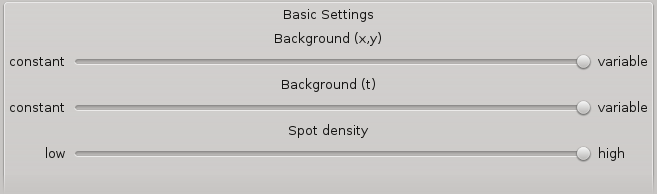
\includegraphics[width = 0.465\textwidth]{pictures/basicSettingsGui1.png}}
\subfloat[Advanced setting widget]{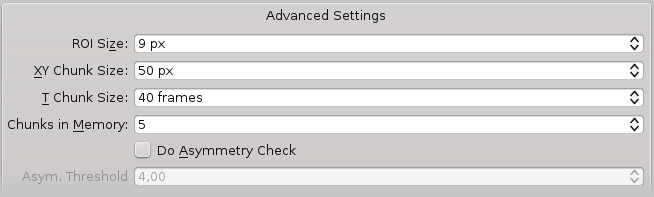
\includegraphics[width = 0.465\textwidth]{pictures/advancedSettingsGui.png}}\hfill
	\caption{There are two different ways to set the parameters for the algorithm. On the right the standard way of setting parameters can be seen. On the left, there are sliders that can be adjusted between the extremes. The program sets the value for the parameters in a way to produce the best results for the selected attributes of the data set.}
	\label{guiSettings}	
\end{figure}
\subsection{Result widget}
After the run button at the lower left edge of the input widget is pressed, a new tab opens. In this widget the reconstructed image is shown. At the bottom there is a progress bar that displays the current processing step and its progress. Buttons to zoom in and out or to fit the displayed image into the window are located in the lower part of the result widget. On the lower right there is the stop/save button. It either stops the program if it is still running or opens a dialog to save the result image and the coordinates of the detection if the program has already been stopped.\newline
The GUI was mainly designed by Ilia Kats.

\begin{figure}
\subfloat[Input widget]{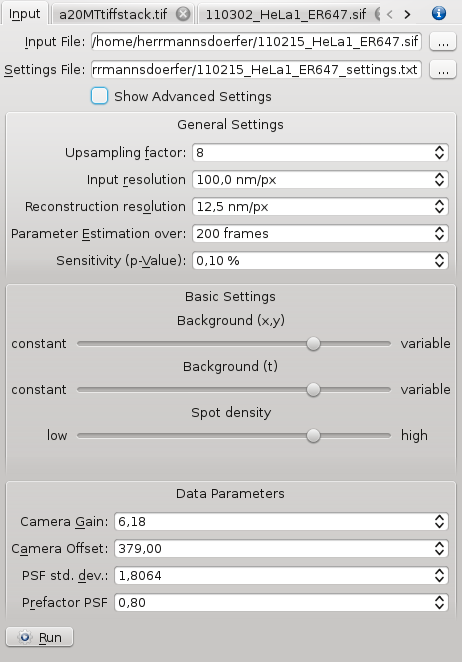
\includegraphics[width = 0.405\textwidth]{pictures/InputWidget.png}}\hfill
\subfloat[Result widget]{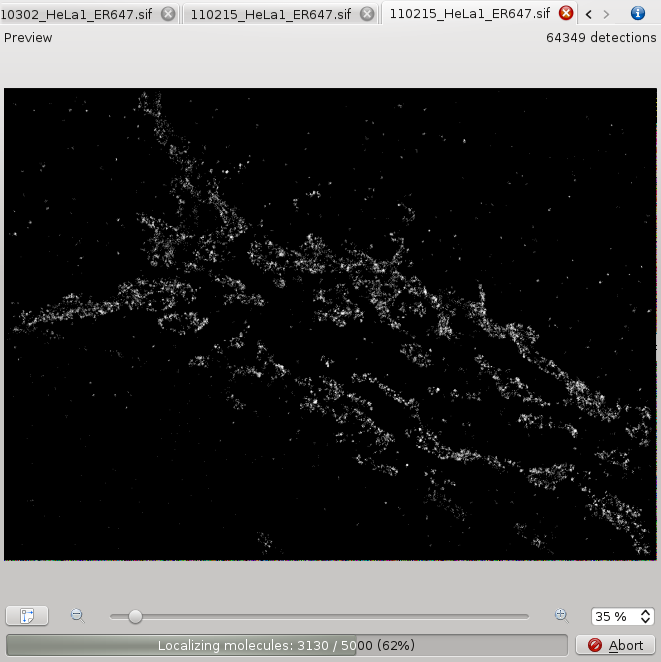
\includegraphics[width = 0.575\textwidth]{pictures/ResultWidget.png}}
	\caption{The new GUI. On the left is the window for selecting input file and parameters. On the right is the result widget showing the processing of a data set in progress.}
	\label{guiWidgets}	
\end{figure}

\subsection{Easy parameter selection}\label{easyParam}
As mentioned above the easy setting widget makes it easy to set reasonable parameters without knowing their influence on the algorithms.\newline
The background sliders have direct influence of the corresponding chunk size. A more constant background gives better results with larger chunks. This is because the median of all pixels in a chunk is used to estimate the mean value of the background. For the estimation of this relation between the median and the mean $\lambda$ of a Poisson distribution, described in equation \ref{meanMedianPoiss}, is used.
Because of the high mean values for $\lambda$ the last summand can be dropped.
This estimation works only if the chunks contain more background pixels than signal, otherwise the mean value will be overestimated. With large chunks this assumption is satisfied. But the smaller the chunk size, the more likely it is that a cluster of points lies in the chunk, and the values of the median are too high. On the other hand, the chunk sizes should be within the range of the changes in background. The best chunksize is therefore in the range of the variable background. The slider position sets the chunk sizes linearly to a value that lies in between the smallest and the largest chunk size possible for the data set.\newline
The minimal possible chunk size is 3 pixels. The largest chunk size possible is half of the shorter border in $x$ and $y$ dimension and the number of frames over which the parameters are estimated divided by the number of chunks in memory in $t$ dimension. These restrictions to the maximal chunk size result from the spline interpolation as described in section \ref{bgestimation}.\newline 
In general, the denser the dataset is, the more likely it is that two neighboring PSFs are merged due to the filtering, as shown in section \ref{sectionFilterisEvil}. There are two ways to avoid inaccurate detections that result from merged PSFs. One is less filtering, to avoid merges, the second one is checking the symmetry of the detected spots. Merged spots become more and more asymmetric the further the two true centers of the PSFs lie apart from each other. A high asymmetry is a good indicator for a detected spot with low accuracy.
The spot density influences the prefactor for the estimated sigma and the value for the asymmetry checks. It sets the threshold for the asymmetry in the same way the sliders for background work, within appropriate limits, with higher values for the asymmetry threshold for less dense data sets. Also, the prefactor is set to values between 1 for sparse data and zero for dense data.
\chapter{Check of the assumptions}
For the whole workflow several assumptions about the data or the results of certain transformations are made. These assumptions have to be met at least roughly to ensure the correctness of the results.\newline
This section gives checks for most of the assumptions like accuracy of the PSF scale estimation or that the matched filter of the matching size compared to the PSF performs best.\newline
Also a discussion about the design choices is present in this chapter.
\section{Calibration measurement}
As described by \cite{meanVar} the gain can be determined using the mean and variance of data with different mean intensities. Therefore a calibration dataset was aquired. The temperature and the gain factor were set to match the settings usually used. A sample with cells was prepared for the Storm measurement. First, eleven time series were taken, with opend shutter and with increasing exposure time from 0 milliseconds up to 1000 milliseconds. Afterwards the same procedure was repeated with the shutter kept closed. Figure \ref{calibplot} shows the results for the first 6 exposure time. All points lie on a straight line. The gain factor determined by the calibration measurement was 3.9, the offset 315. This offset is too small. An other method was used to determine the offset. There were also an other series of  images taken with closed shutter. This series shows the response of the camera without any light around. The mean value of the shortest exposure time was taken as offset. Its value is 380. 
\begin{figure}
\centering
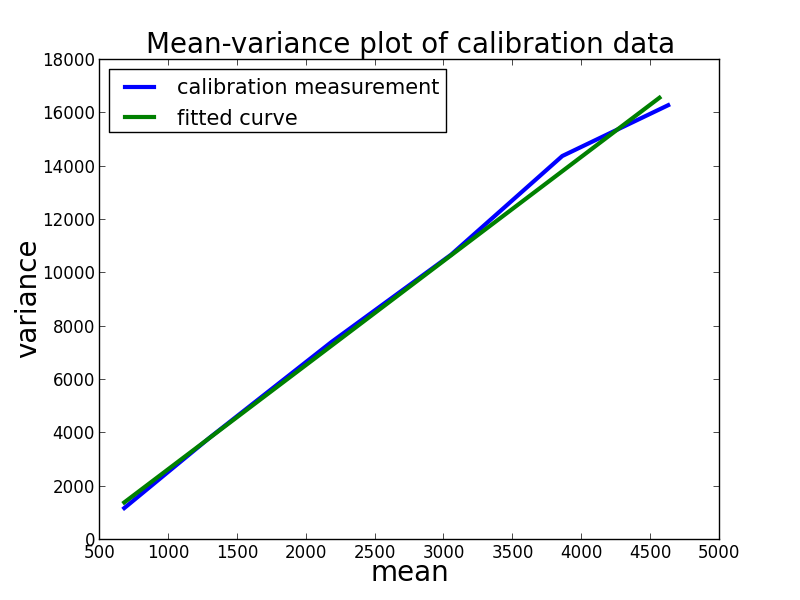
\includegraphics[width = 0.88\textwidth]{pictures/meanVariancePlotCalibration.png}
	 \caption{Result of the calibration measurements. The gain determined from this variance-mean plot is 3.9.}
	\label{calibplot}
\end{figure}


\section{Correction to Poisson distributions}
It is very important for the whole workflow that the first transform results in background intensities that follow a Poisson distribution. To test this, a real world image was transformed with parameters taken from the calibration measurement described in the previous section. The offset was estimated from the minimal intensity of the raw image. The histograms for two generic background pixels are shown in Figure \ref{isitPoisson}. A Poisson distribution with the mean of the pixels intensities is also shown in the figures. These histograms were aquired using the pixel intensities of one pixel for 3000 frames. The histogram matches the expected Poisson distribution.
\begin{figure}
\subfloat[Tubulin2 frame 10]{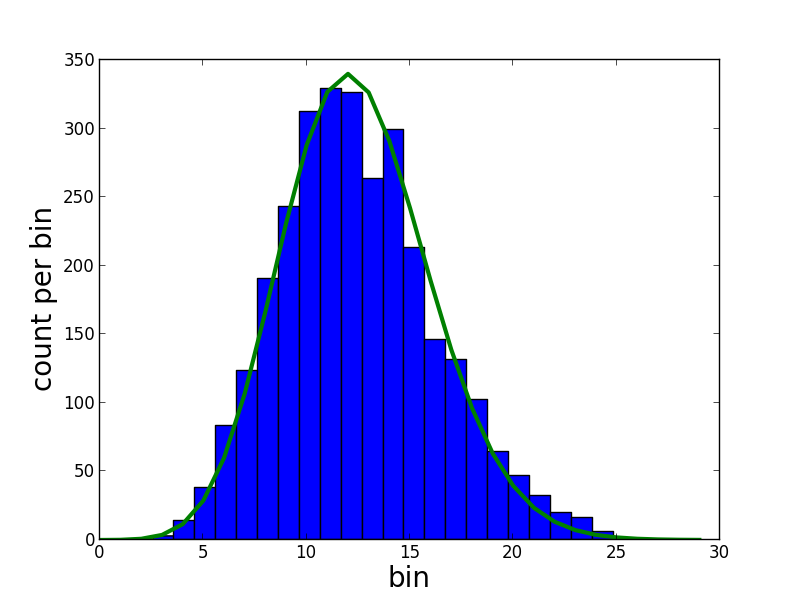
\includegraphics[width = 0.485\textwidth]{pictures/IsItPoisson105_105.png}}\hfill
\subfloat[Tubulin2 frame 1010]{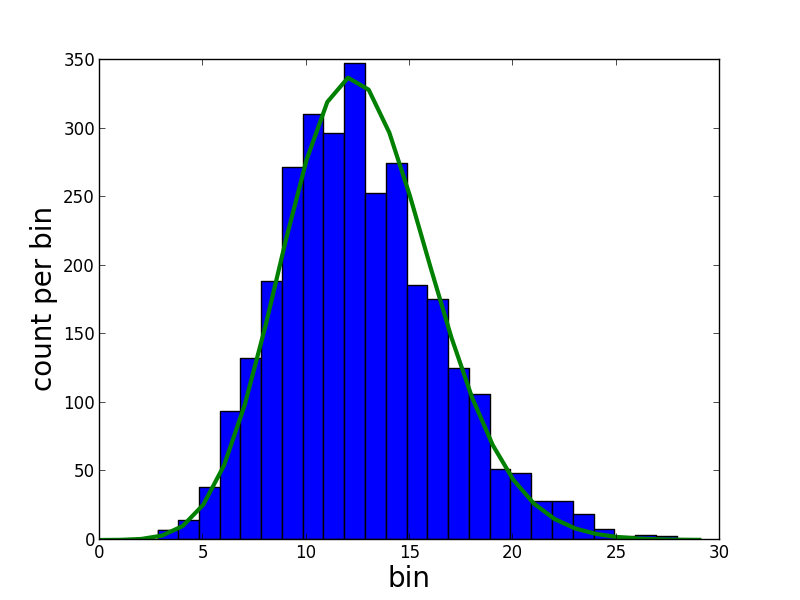
\includegraphics[width = 0.485\textwidth]{pictures/IsItPoisson50_50.png}}
	\caption{These pictures show how well the histograms of background pixels taken over the first 3000 frames, follow a Poisson distribution. For the gain the parameter from the calibration measurement of $g$ = 3.9 was used. The offset was estimated from the minimal intensities of the original image.}
	\label{isitPoisson}	
\end{figure}

\section{Result Anscombe transformation}
After the transformation described in \ref{trafoPoiss}, the Anscombe transformation was aplied on the same data set that was used in the previous section and the background was subtracted. Figure \ref{isitAnscombe} shows the histogram of the intensities of one randomly chosen frame and a Gaussian with zero mean and unit variance. The histogram fits very well to the Gaussian. The tail exceeding the Gaussian on the right side can at least partially be explained by the signal that is present in the image and does not follow the Gaussian distribution, but has higher intensities.\newline
\begin{figure}
\centering
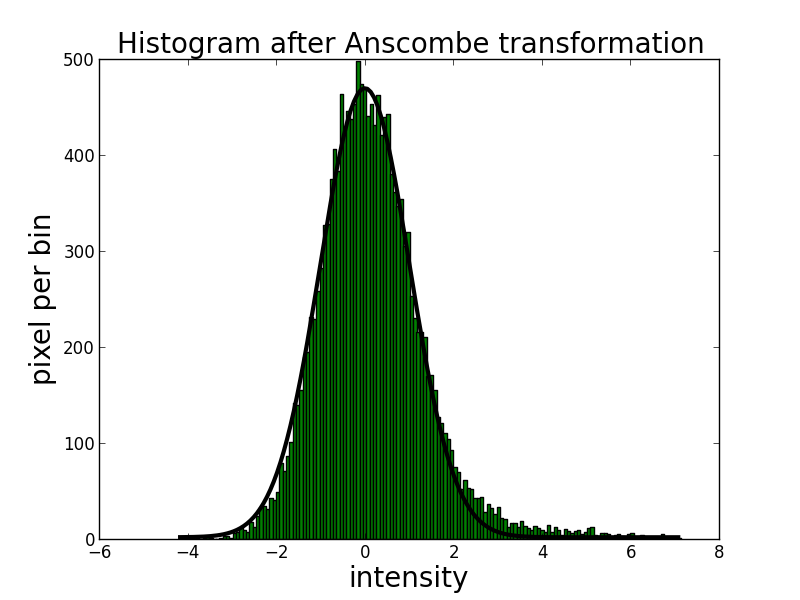
\includegraphics[width = 0.88\textwidth]{pictures/anscombeAndFit.png}
	 \caption{After the Anscombe transformation the background pixel intensities should be distributed with mean zero and variance one. This figure shows the histogram of the pixel intensities and a fitted Gaussian with variance one and mean zero.}
	\label{isitAnscombe}
\end{figure}
There may be confusion why the Anscombe transformation that is applied to all intensities of one time step instead of all intensities of one pixel, does work. This is because the Anscombe transformation is applied to each intensity independently. Therefore all intensities at a certain time step are one sample from the Gaussian distribution in $t$ dimension that results from the Anscombe transformation. All of these Gaussian distributions in $t$ dimension have the same mean (since the background was subtracted) and variance. This means that the distribution created from all intensities of a certain frame has the same mean and variance as the transformed Poisson distributions in $t$ dimension.
\section{Accuracy of detection}
Unfortunately the position of the flourescent molecules can not be detected
perfectly. There are two main contribution to the errors in detection.\\
On one hand, there is a problem with finding the maximum in a noisy signal. Due to
noise the spots maxima might be shifted.\newline
On the other hand, the position of the fluorescent molecule is deteted by upscaling the pixel grid and interpolation.
After that the maximums position of the upscaled grid is taken as the resulting
position. This gives an error from roughly a 12th pixelwidth. This error becomes less important with higher upscaling factors.\newline

Because there is no groundtruth for the real data, test data and groundtruth had to be produce. This was done similar to the method described by \cite{simulated}. The difference was, that instead of generating just one spot per frame a different number of spots were simulated for each frame. For different signal-to -noise ratios, a dataset with 40 times 40 pixels and 1000 frames was created. Each frame containing one, three or five point spread functions. The position of the spots was determined beforehand, to use the same spots for each signal to noise ratio.\newline

To determine the accuracy, the standard deviation between the true position of the signal and its detection were used. For data sets with more than one spot per frame, the best match within a certain distance around the true position was found. If a pair of true spot and detection were found, both were removed for further matching of the remaining signals. In the end the averaged standard deviation of the detection relative to the true positions were calculated as follows:
\begin{align}
	\text{std. dev.} = \sum_i \sqrt{\left(\bf{p}_{\text{true}}^i - \bf{p}_{\text{detec}}^i\right)^2}
\end{align}
$i$ runs over all found pairs of groundtruth and detections, $\bf{p}$ describes the two dimensional spatial vector of the groundtruth or detection respectivly.\newline

The results can be seen in Figure \ref{accplot}. The Figure shows, that the more spots are present per frame the harder it is to detect them properly. This is a result of the fact that spots that lay near each other might be detected as one spot. This gives rise to higher errors in the detection accuracy.


\begin{figure}
\begin{minipage}[t]{0.48\textwidth}
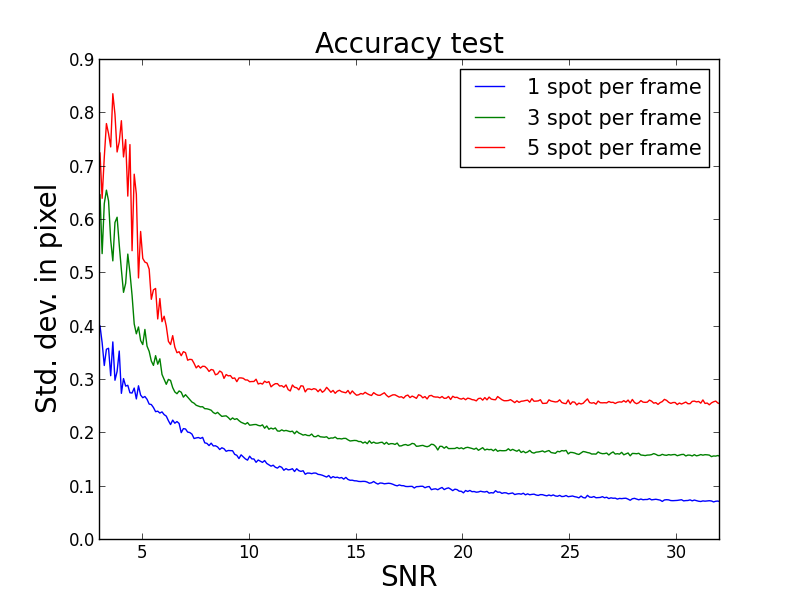
\includegraphics[width = 0.99\textwidth]{pictures/AccuracyTest.png}
	\caption{Result of the accuracy test. For datasets with one, three or five point spread functions per frame, evaluated for different signal to noise levels. The more dense the spots are the less accurate the detections are.}
	\label{accplot}	
\end{minipage}\hfill
\begin{minipage}[t]{0.48\textwidth}
\centering
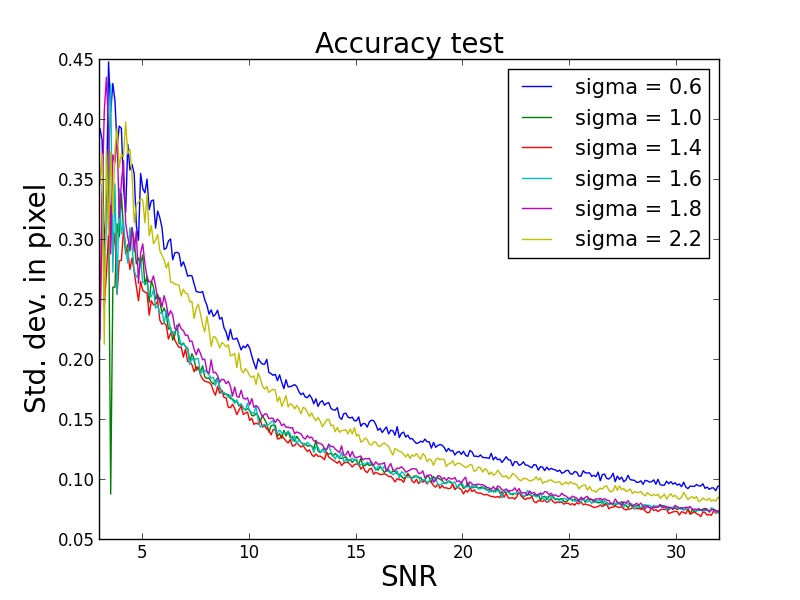
\includegraphics[width = 0.99\textwidth]{pictures/AccuracyTestSigma.png}
	\caption{Result of the accuracy test for different sigmas for the Gaussian smoothing. One data set was processed with different sigma values and evaluated for different signal to noise levels. The true standard deviation of point spread function of the simulated data is 1.4.}
	\label{accplot2}

\end{minipage}
\end{figure}


\section{Matched filter is best filter} \label{detectionError}
For denoising the image a matched filter is used. Since it is assumed that the point spread function is Gaussian, a two dimensional Gaussian filter with the estimated size of the point spread function is used. The following calculation shows why this is the best choice for the standard deviation.\newline
This calculation was inspired by the calculation in \cite{ulli}, page 207.\newline 
The assumptions are, the point spread function is Gaussian shaped with a true standard deviation of $\sigma_\text{PSF}$, the image contains white Gaussian noise with mean zero and unit variance, the applied filter for denoising is a Gaussian filter with standard deviation $\sigma_\text{filter}$.\newline
The image $f$ is composed of Gaussian filter convolved with the signal $s$ and the above mentioned white noise $n$. $s$ and $n$ describe the filtered signal respectivly noise.
\begin{align}
 f=s+n \label{gl91}
\end{align}
Without noise the first derivative of $f$ which is equal to $s$ in the noise-free case vanishs at the center of the Gaussian signal. This center can be set to the origin without losing generality. But noise shifts the zero crossing of the first derivatives to $\Delta x,~\Delta y$. For now just one dimension is considered.
\begin{align}
\frac{\partial f}{\partial x}\left(\Delta x, \Delta y\right) &= \frac{\partial s}{\partial x} \left(\Delta x, \Delta y\right) + \frac{\partial n}{\partial x}\left(\Delta x, \Delta y\right)&=0
\end{align}  

Using Taylor expansion around $x = 0$ at $y= 0$ for the signal, yields:
\begin{align}
f_x(\Delta x, \Delta y)&\approx \underbrace{s_x(0, 0)}_{=0} + s_{xx}(0, 0)\cdot \Delta x + n_x(\Delta x, \Delta y)&=0\\
\Rightarrow \text{var}(s_{xx}(0, 0)\cdot \Delta x)&= \text{var}(n_x(\Delta x,\Delta y)\\
\Rightarrow \text{var}(\Delta x) &= \frac{\text{var}(n_x(\Delta x, \Delta y)}{s_{xx}^2(0, 0)} \label{ch9gl1}
\end{align}

The result for the variance of the first derivative of white noise convolved with a Gaussian filter of width $\sigma_\text{filter}$ can be found at \cite{ulli}, page 204. It is:
\begin{align}
	\text{var}(n_x) = \frac{N^2}{8\pi\sigma_\text{filter}^4},~\text{with }N\text{: noise std. dev} \label{ch9gl2}
\end{align}
The convolution of the Gaussian PSF  with an other Gaussian results in Gaussian with combined scales.
\begin{align}
 \mathcal{N}(0,\sigma_\text{PSF}) \ast \mathcal{N}(0,\sigma_\text{filter}) = \mathcal{N}\left(0,\underbrace{\sqrt{\sigma_\text{PSF}^2+\sigma_\text{filter}^2}}_{=\sigma_\text{comb}}\right)
\end{align}
The value of the second derivative in $x$-direction of the convolved PSF at (0,0) is:
\begin{align}
 \frac{\partial^2 S_0\cdot\mathcal{N}\left((\mu_x,\mu_y),\sigma_\text{comb}\right)}{\partial x^2}  &=  -\frac{S_0}{2\pi \sigma_\text{comb}^4}  \label{ch9gl3}
\end{align}
Combining \ref{ch9gl1}, \ref{ch9gl2} and \ref{ch9gl3} yields:
\begin{align}
\text{var}\left(\Delta x\right) &= \dfrac{\dfrac{N^2}{8\pi\sigma_\text{filter}^4}}{\dfrac{S_0^2}{4\pi^2 \sigma_\text{comb}^8}}\\
&= \frac{N^2\cdot 4\pi^2 \sigma_\text{comb}^8}{S_0^2\cdot8\pi\sigma_\text{filter}^4}\\
&= \frac{N^2}{S_0^2} \frac{\pi \left(\sigma_\text{filter}^2+\sigma_\text{PSF}^2\right)^4}{2\sigma_\text{filter}^4}\\
&= \frac{N^2\pi}{2S_0^2} \left(1+\frac{\sigma_\text{PSF}^2}{\sigma_\text{filter}^2}\right)^2\left(\sigma_\text{filter}^2+\sigma_\text{PSF}^2\right)^2 
\end{align}
The same calculation can be done with respect to $y$. This gives the same variance, yielding a total variance that is square root of 2 times larger, because the variances are orthogonal.
Therefore the standard deviation of the localization is:
\begin{align}
 \text{std. dev loc}&=\frac{N}{S_0}\sqrt{\frac{\sqrt{2}\pi}{2}}
 \left(1+\frac{\sigma_\text{PSF}^2}{\sigma_\text{filter}^2}\right)\left(\sigma_\text{filter}^2+\sigma_\text{PSF}^2\right) 
\end{align}
To verify these results test data sets have been created containing 3500 frames with one PSF per frame. Each created data set contained a PSF with different scale. This data sets have been filtered with Gaussian filters of different sizes. After that the maximum for each frame was detected and compared with the true position. Figure \ref{matchedFilter1} shows the accuracy for different PSF scales and filter widths.\newline
The best results were achieved using a Gaussian filter with the PSFs size. The larger the PSFs scale the more inaccurate the localization becomes.\newline

\begin{figure}
\centering
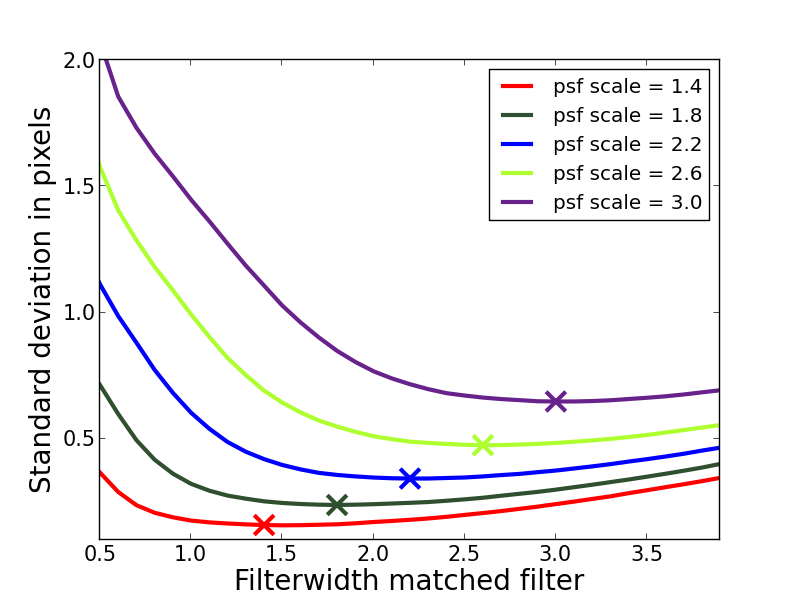
\includegraphics[width = 0.88\textwidth]{pictures/matchedFilterPlots1.png}
	 \caption{This figure shows the accuracy of detection achieved using different Gaussian filters for denoising. The cross marks the minimum of each curve.}
	\label{matchedFilter1}
\end{figure}

The figures in \ref{matchedFilter2} show the measurement, a shifted measurement curve and the result of the calculation. The measured error was larger than the calculated error, therefore the shifted line is also shown to state that the curves shape match but there is an additional error that shifts the line. \newline
These results show that the calculated standard deviation of the localization can be used to estimate the localization error of SimpleSTORM for further calculations or error propagation.

\begin{figure}
\subfloat[PSFs scale = 2.6]{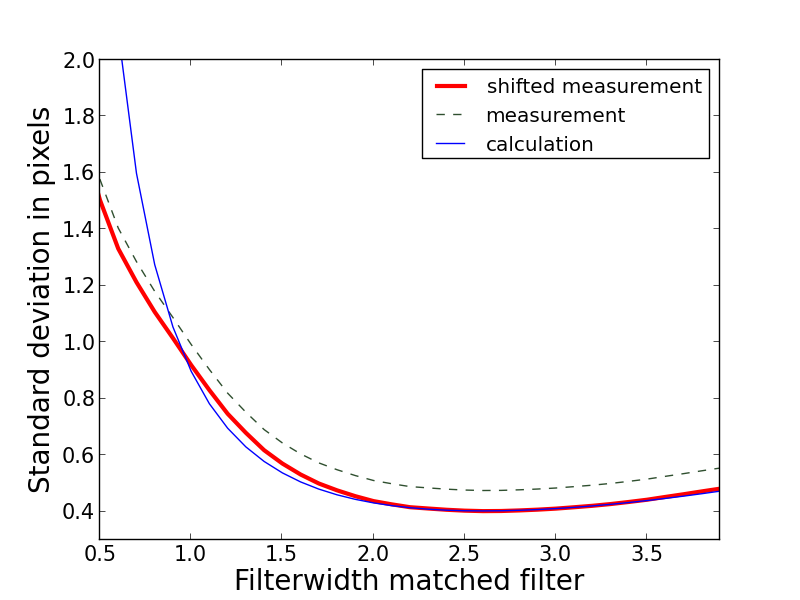
\includegraphics[width = 0.485\textwidth]{pictures/matchedFilterPlots2.png}}\hfill
\subfloat[PSFs scale = 1.8]{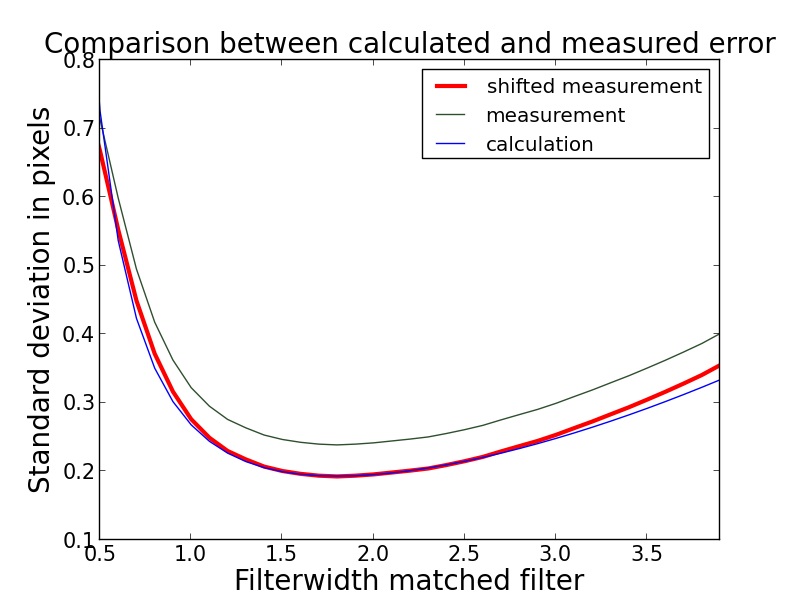
\includegraphics[width = 0.485\textwidth]{pictures/matchedFilterPlots3.png}}
	\caption{Comparison between the measured and the calculated localization error. The dashed lines show the unchanged measurement results, for better comparism the line was shifted to match the calculated error.}
	\label{matchedFilter2}	
\end{figure}

\section{Test PSF estimation}
The estimation of the width of the point spread function of the signal is very important. The localization error increases with larger deviations of the matched filters width from the true width of the PSF, as shown in \ref{detectionError}. \newline
Figure \ref{estimatedSigma} shows the results of an accuracy test. For this test, data was created artificially. One PSF was simulated at a random location with a fixed width, poisson noise was added. The signal-to-noise ratio was set to 10. Then this width was estimated by the SimpleSTORM algorithm. This was done with values for the standard deviation of the Gaussian in a range from 0.2 up to 4. The plot shows that for standard deviations up to 2.5 the estimated value for the width is very close to the actual value. The wider the PSF becomes in the spatial domain the smaller it gets in the Fourier domain. This is the reason why the accuracy of the estimation is decreasing for larger widths. This effect can be reduced by choosing a larger region of interest for the power spectrums acumulation. The parameter chosen for the plot in figure \ref{estimatedSigma} was the default value. The typical width of the PSF for real world data is in a range of 1 to 2, this is a range in which the estimation gives reliable results.\newline
\begin{figure}
\centering
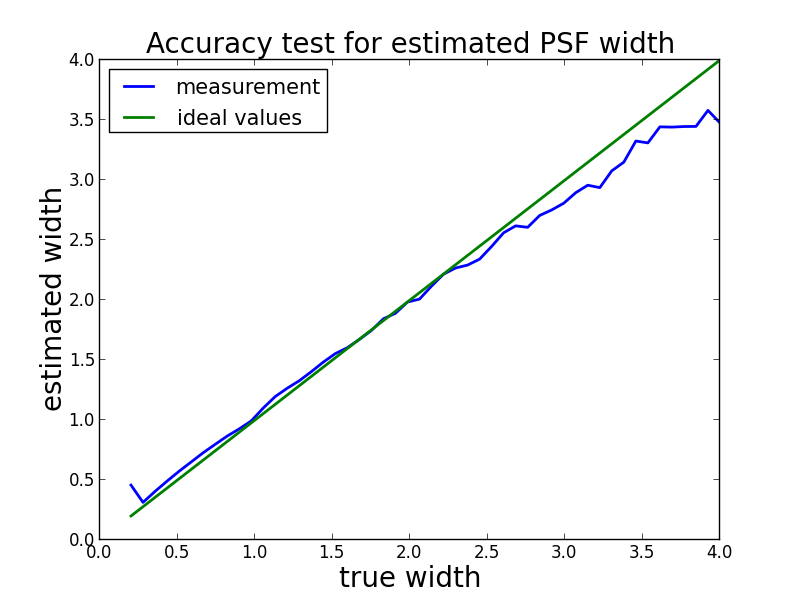
\includegraphics[width = 0.88\textwidth]{pictures/AccuracyTestPSFWidth.png}
	 \caption{The figure shows the estimated widths of the point spread function plotted over the true widht of the simulated signal. The signal-to-noise ratio was 10 for this test. The green line shows the simulated values.}
	\label{estimatedSigma}
\end{figure}


\section{Bleaching signal}
One assumption was that the backgrounds illumination is caused mainly from out of focus fluorophors and is therefore Poission distributed. If this is the case the background illumination should decrease over time. Bleaching of fluorophores describes the process in which the fluorescent molecules change their conformation and lose the ability to emit light permanently. The spectrum of the emission can also change so that the fluorescent molecules can not be detected any more. All fluorophores used for the STORM images available to us bleach over time. This decay of the mean backgrounds intensity is shown in figure \ref{bleaching}.

\begin{figure}
\centering
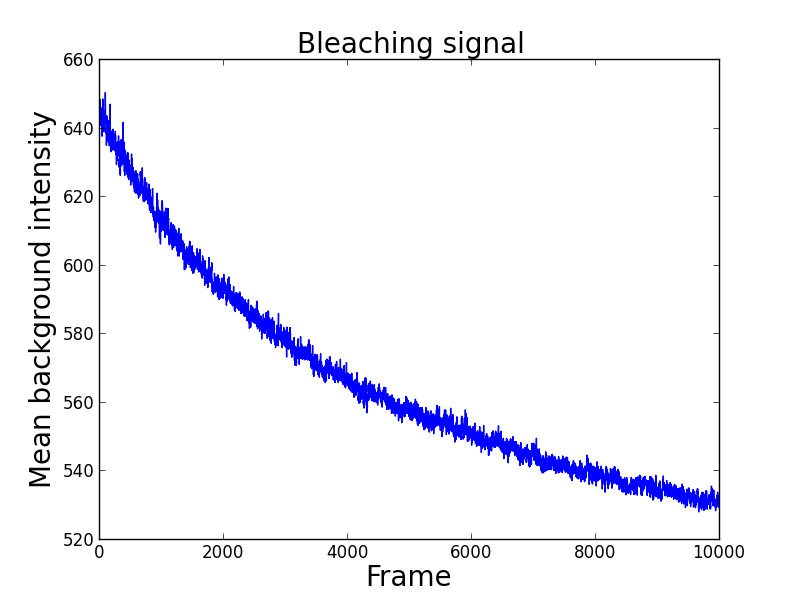
\includegraphics[width = 0.5\textwidth]{pictures/bleaching.png}
	\caption{The number of active fluorophores decreases over time and so does the mean intensity of the image. This picture shows the mean intensities of 10 background pixel over time. }
	\label{bleaching}
\end{figure}

\section{Reliability of skewness estimation} \label{skewnesssucks}
To estimate the true Poisson distributions mean using its skewness is a direct way to get to the true distribution regardless of the camera parameters.\newline
This approach has one drawback. The larger the mean value of a Poisson distribution gets, the more similar the Poisson distribution gets to a Gaussian. This means that the skewness, which measures the assymetry of the distribution gets smaller and smaller, converging to zero. The inverse of the skewness squared is used to estimate the mean of the Poisson distribution, this means that small uncertainties for the skewness lead to a high uncertainty for the estimated mean. Also a single distribution with a couple of hundred samples yields no reliable estimate. A robust estimate can be achieved if the median of several distributions is calculated. Figure \ref{skew1000} show the results of the estimate of the mean using the skewness approach on patches of different size. The plot shows the estimated value on the ordinate, the true value on the abscissa. The different lines show the results for different sizes of the distribution. Figure \ref{skew100} shows the same plot but for smaller distribution sizes.

\begin{figure}
\subfloat[10 times 10 pixel patch]{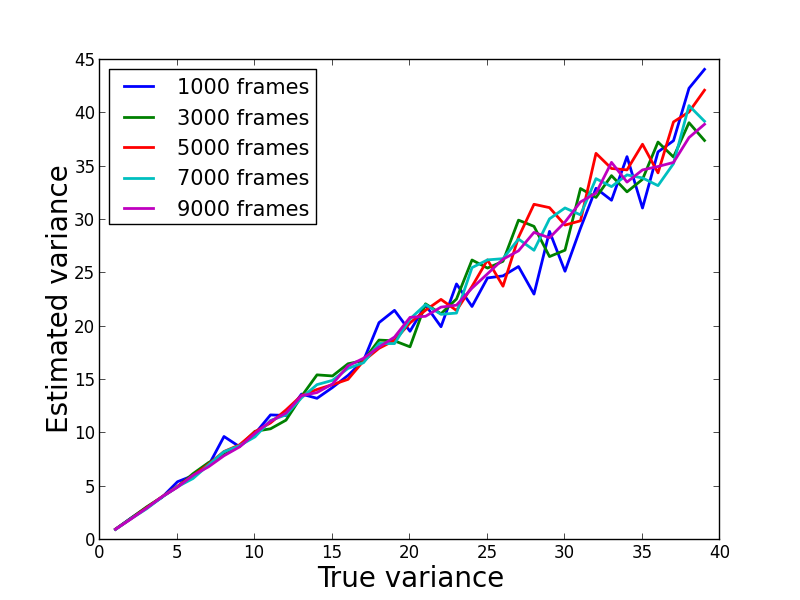
\includegraphics[width = 0.485\textwidth]{pictures/skewness100.png}}\hfill
\subfloat[20 times 20 pixel patch]{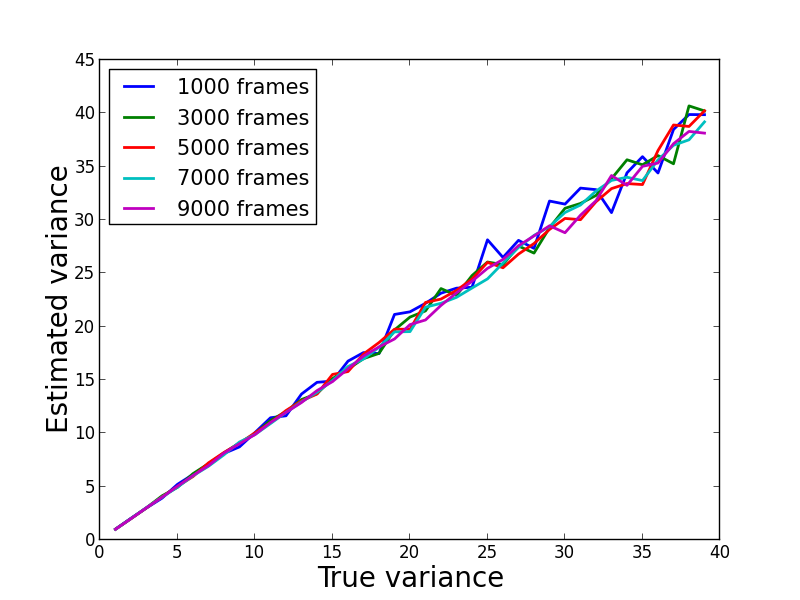
\includegraphics[width = 0.485\textwidth]{pictures/skewness400.png}}
	\caption{Result of mean estimation using skewness approach.}
	\label{skew1000}	
\end{figure}
\begin{figure}
\subfloat[10 times 10 pixel patch]{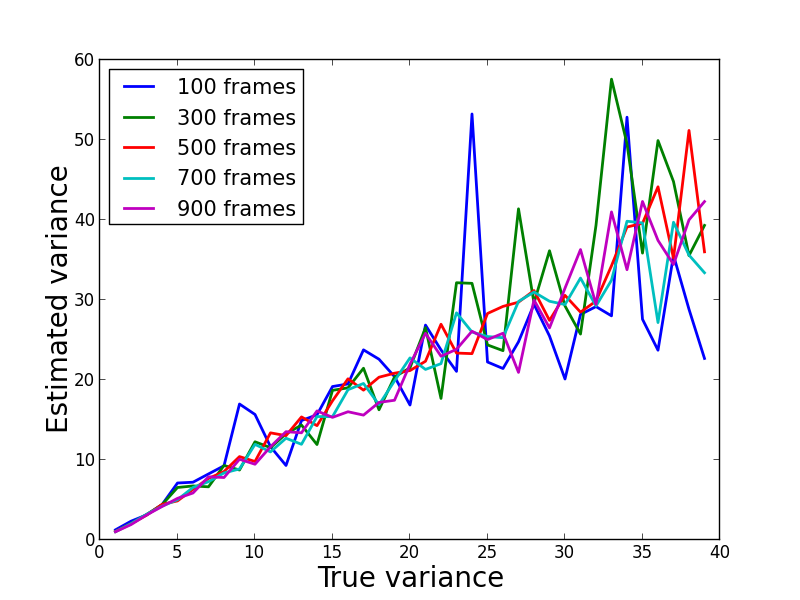
\includegraphics[width = 0.485\textwidth]{pictures/skewness2100.png}}\hfill
\subfloat[20 times 20 pixel patch]{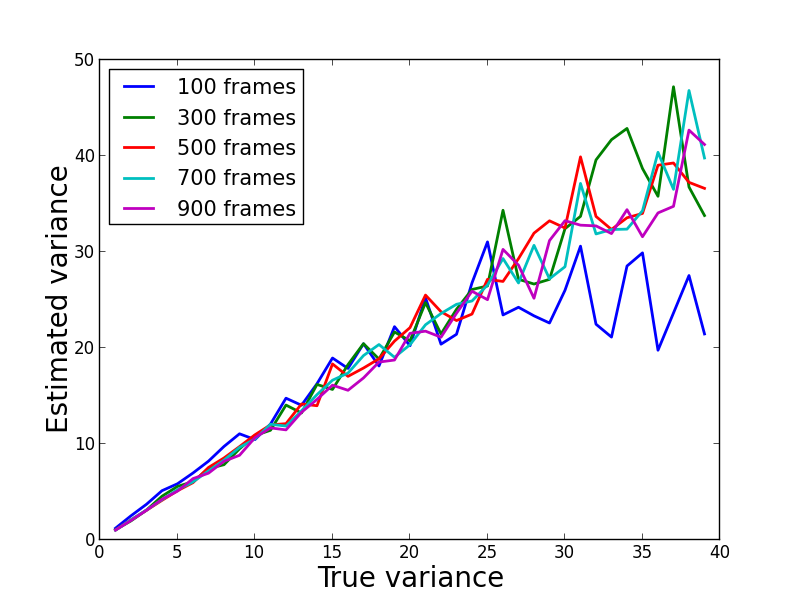
\includegraphics[width = 0.485\textwidth]{pictures/skewness2400.png}}
	\caption{Result of mean estimation using skewness approach.}
	\label{skew100}	
\end{figure}
The estimate for the mean is accurate even for a smaller number of samples up to 15 to 20.\newline
This approach has the drawback that for small data sets with only several hundred frames the accuracy of the estimated values is low. An other problem are artificially created data sets with a background intensity of 100 or above. In that case the skewness approach gives no reliable results.

\section{Points lie above desired line}\label{pointsabove}
To estimate the camera gain and offset from the raw data the method described in \ref{skellam1} is used. Ideally the intensities for every pixel would follow a Poisson distribution with a certain mean. However this assumption only holds for beads and background pixel that never show any signal. The resulting points in the variance over mean plot will lie on a straight line. But what happens if background pixels are illuminated by a fluorophore in one or several frames?\newline
This section proves that points in the variance over mean intensity plot lie on the straight line or above, but almost never below.\newline
Set $A$ contains $n$ samples drawn from a Poisson distribution. The variance and mean of the set shall be $\mu_p$. Set $B$ is equal to set $A$ but the last ($n^\text{th}$) member $p_n^A$ is replaced by $p_n^A+c$. $c$ is a positive value that describes the difference in intensity between a background pixel and an illuminated pixel.\newline  

The exchange of the last pixel increased the mean intensity:
\begin{align}
\mu_B&=\frac{1}{n}\sum_{i=1}^n(p_i^B)\\
&=\frac{1}{n}\left(\sum_{i=1}^{n-1}(p_i^A) +p_n^A+c \right)\\
&=\frac{1}{n}\left(\sum_{i=1}^{n}(p_i^A) +c \right)\\
&=\mu_p + \frac{c}{n}
\end{align}
The variance of set $B$ times $(n-1)$ is given as:
\begin{align}
(n-1)\cdot\text{var}(B)&=\sum_{i=1}^n \left(p_i^B - \left(\mu_p+\frac{c}{n}\right)\right)^2\\
&=\sum_{i=1}^n \left(\left(p_i^B\right)^2 - 2p_i^B\mu_p-\frac{2p_i^Bc}{n}+\left(\mu_p+\frac{c}{n}\right)^2\right)\\
&=\sum_{i=1}^n \left(\left(p_i^B\right)^2 - 2p_i^B\mu_p+\mu_p^2 -\frac{2p_i^Bc}{n}+\frac{2c\mu_p}{n}+\frac{c^2}{n^2}\right)\\
&=\sum_{i=1}^{n-1} \Big(\underbrace{\left(p_i^A\right)^2}_{=p_i^B \text{for } i\neq n} - 2p_i^A\mu_p+\mu_p^2\Big)+\underbrace{\left(p_n^A+c\right)^2}_{=\left(p_n^B\right)^2} -2\left(p_n^A+c\right)\mu_p + \mu_p^2 \\
&~~+\sum_{i=1}^n\left(-\frac{2p_i^Bc}{n}+\frac{2c\mu_p}{n}+\frac{c^2}{n^2}\right) \nonumber\\
&=\sum_{i=1}^{n} \left(\left(p_i^A\right)^2 - 2p_i^A\mu_p+\mu_p^2\right)+2p_n^Ac+c^2-2c\mu_p\\
&~~+\sum_{i=1}^n\left(-\frac{2p_i^Bc}{n}+\frac{2c\mu_p}{n}+\frac{c^2}{n^2}\right) \nonumber\\
%&=(n-1)\mu_p+2p_n^Ac+c^2-2c\mu_p+\sum_{i=1}^n\left(-\frac{2p_i^Bc}{n}+\frac{2c\mu_p}{n}+\frac{c^2}{n^2}\right)\\
&=(n-1)\mu_p+2p_n^Ac+c^2+\frac{c^2}{n}-\sum_{i=1}^n\frac{2\left(p_i^B\right)c}{n}\\
&=(n-1)\mu_p+2p_n^Ac+c^2+\frac{c^2}{n}-\sum_{i=1}^{n-1}\frac{2\left(p_i^A\right)c}{n} -\frac{2\left(p_n^A+c\right)c}{n}\\
&=(n-1)\mu_p+2p_n^Ac+c^2+\frac{c^2}{n}-\sum_{i=1}^{n}\frac{2\left(p_i^A\right)c}{n} -\frac{2c^2}{n}\\
&=(n-1)\mu_p+2p_n^Ac+c^2+\frac{c^2}{n}-2c\mu_p -\frac{2c^2}{n}\\
&=(n-1)\mu_p+2c\left(p_n^A-\mu_p\right)+c^2 \left(1-\frac{1}{n}\right)
\end{align}
The exchange of $p_n^A$ increased the mean intensity, the variance of $B$ must exceed $\mu_p+1/n$ to lie above the line. Therefore the second part of the sum in equation \ref{gliwa} must be larger than $1/n$.
\begin{align}
\text{var}(B)&=\mu_p+\underbrace{\frac{2c\left(p_n^A-\mu_p\right)+c^2 \left(1-\frac{1}{n}\right)}{n-1}}_{>\frac{1}{n}}\label{gliwa}\\
&~~\frac{1}{n-1}\Big(2c\underbrace{\left(p_n^A-\mu_p\right)}_{> -\mu_p}+c^2 \left(1-\frac{1}{n}\right)\Big)&\overset{!}{>}\frac{1}{n}\\
\Rightarrow c &>\frac{\sqrt{\left(\mu_p^2+1\right)n^2-2n+1}+\mu_pn}{n-1}
\end{align}
\begin{align}
\frac{\sqrt{\mu_p^2n^2+n^2-2n+1}+\mu_pn}{n-1}&=\frac{\sqrt{\mu_p^2n^2+(n-1)^2}+\mu_pn}{n-1}\\
&\leq \frac{2\mu_p n}{n-1}+1 ,\text{because $\mu_p, n>0$ and $n>2$}\\
&< 2\mu_p + 1
\end{align}
This result confirms that if the additional intensity caused by signal $c$ is at least two times the mean intensity plus one, the pixels variance rises.\newline
If $n$ samples from a Poisson distribution with mean $\mu_p$ are drawn, and one sample has the lowest value possible, for a Poisson distribution, one, at least two times the mean value has to be added to increase the variance. Lower values for $c$ would decrease the summand $(p_n - \mu_p)^2$. The mean of the set increases if the replaced value lies further apart from the mean after replacement than before.\newline
The variance increses even stronger when the pixel is illuminated by a fluorophore more than once. The variance is not affected by a constant offset, but increases even more rapidly if a gain factor larger than one is present. In case of a gain factor $g$ the equations would get multiplied by $g^2$.\newline

Figure \ref{simulatedScatter} shows a scatter plot of simulated data. For this plot a normal data set with 200 frames were simulated. The data set contains background pixel with mean intensitie between five and ten and beads with intensities between 80 and 160. For each pixel a Poisson distribution with the given mean is drawn. 30 PSFs per frame with a standard deviation of two and an intensity of 80 were added. The data was multiplied by 4 and an offset of 400 was added. Only a subset of all points is plotted. In Figure \ref{simulatedScatter} the blue line shows the expected position for pixels with constant intensity. Pixels that were not affected by any signal are displayed as green dots. The color of all the other pixel is calculated based on the value $c$ added by the PSF. A red color is used if the added $c$ is larger than the mean intensity, a blue color is used if the additional intensity is lower than the mean value of the pixel. The brighter the dots are the more often they are affected by signal. It can be seen, that the points tend to lie above the line, even when less than the mean value is added.
\begin{figure}
\centering
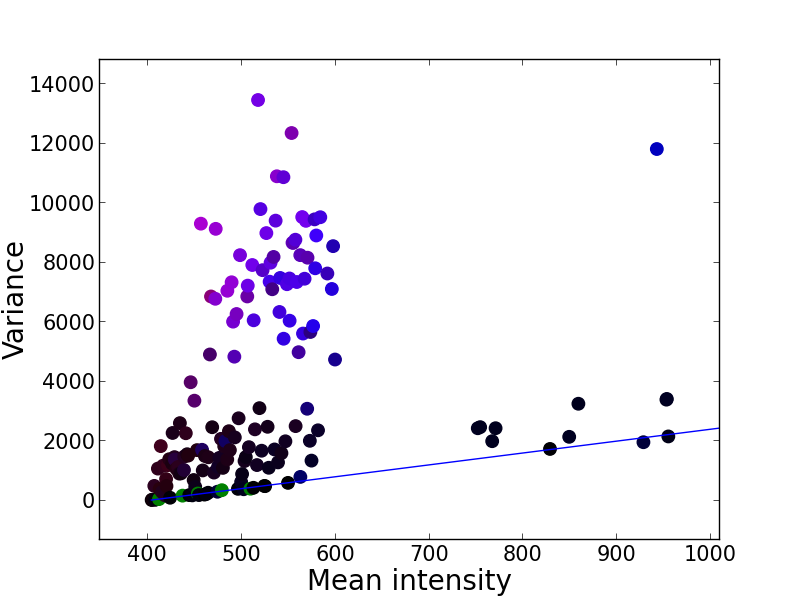
\includegraphics[width = .7\textwidth]{pictures/scatterplot_psfint_2000intmax_80_resx_150psfw_2.png}
\caption{Variance mean scatter plot. The blue line indicates where pixels with constant mean would be displayed.}\label{simulatedScatter}
\end{figure}

\section{Variance vs Skellam}\label{skellambettervariance}
For the estimation of the camera gain and offset the method described in section \ref{estimationCameraGain} is used. There are two different ways to estimate the variance of pixel intenensities.\newline
The variance can be computed directly or the Skellam distribution as described in section \ref{skellamdist} can be used.\newline
The problem is to estimate the variance of the Poisson distribution of the pixels as good as possible, with as few samples as possible. The condition to work well on as few frames as possible araises, because there may be data sets with only 200 or 300 frames or the user does not want to spend more time on the parameter estimation.\newline
To test which method for the variance estimation performs best, from a Poisson distribution with variance one, 200 samples are drawn, multiple times. Both methods were used to estimate the true variance. From all estimations the mean value of the estimated variance and the variance of the estimated variance were calculated. After that the procedure was repeated with increased true variance.\newline
Figure \ref{skellamvarmean} shows the results of for the mean of the estimated variances, Figure \ref{skellamvarvar} shows the variance of the estimated variances, plotted over the true variance of the Poisson distribution.\newline
Figure \ref{skellamvarmean} shows, the mean estimates for the variance of a Poisson distribution with variances between zero and 40. The mean of all estimates from the Skellam approach is almost the same as the true variance (a straight line with slope one and zero intercept). The variance approach underestimates the true variance. Figure \ref{skellamvarvar} shows the variances of the estimates for both approaches. The variance approach has a lower variance than the Skellam approach.\newline
Only one estimate is calculated in practice, therefore the variance approach is taken, because of the lower variance for the estimated values.

%\begin{figure}
%\begin{minipage}{0.48\textwidth}
%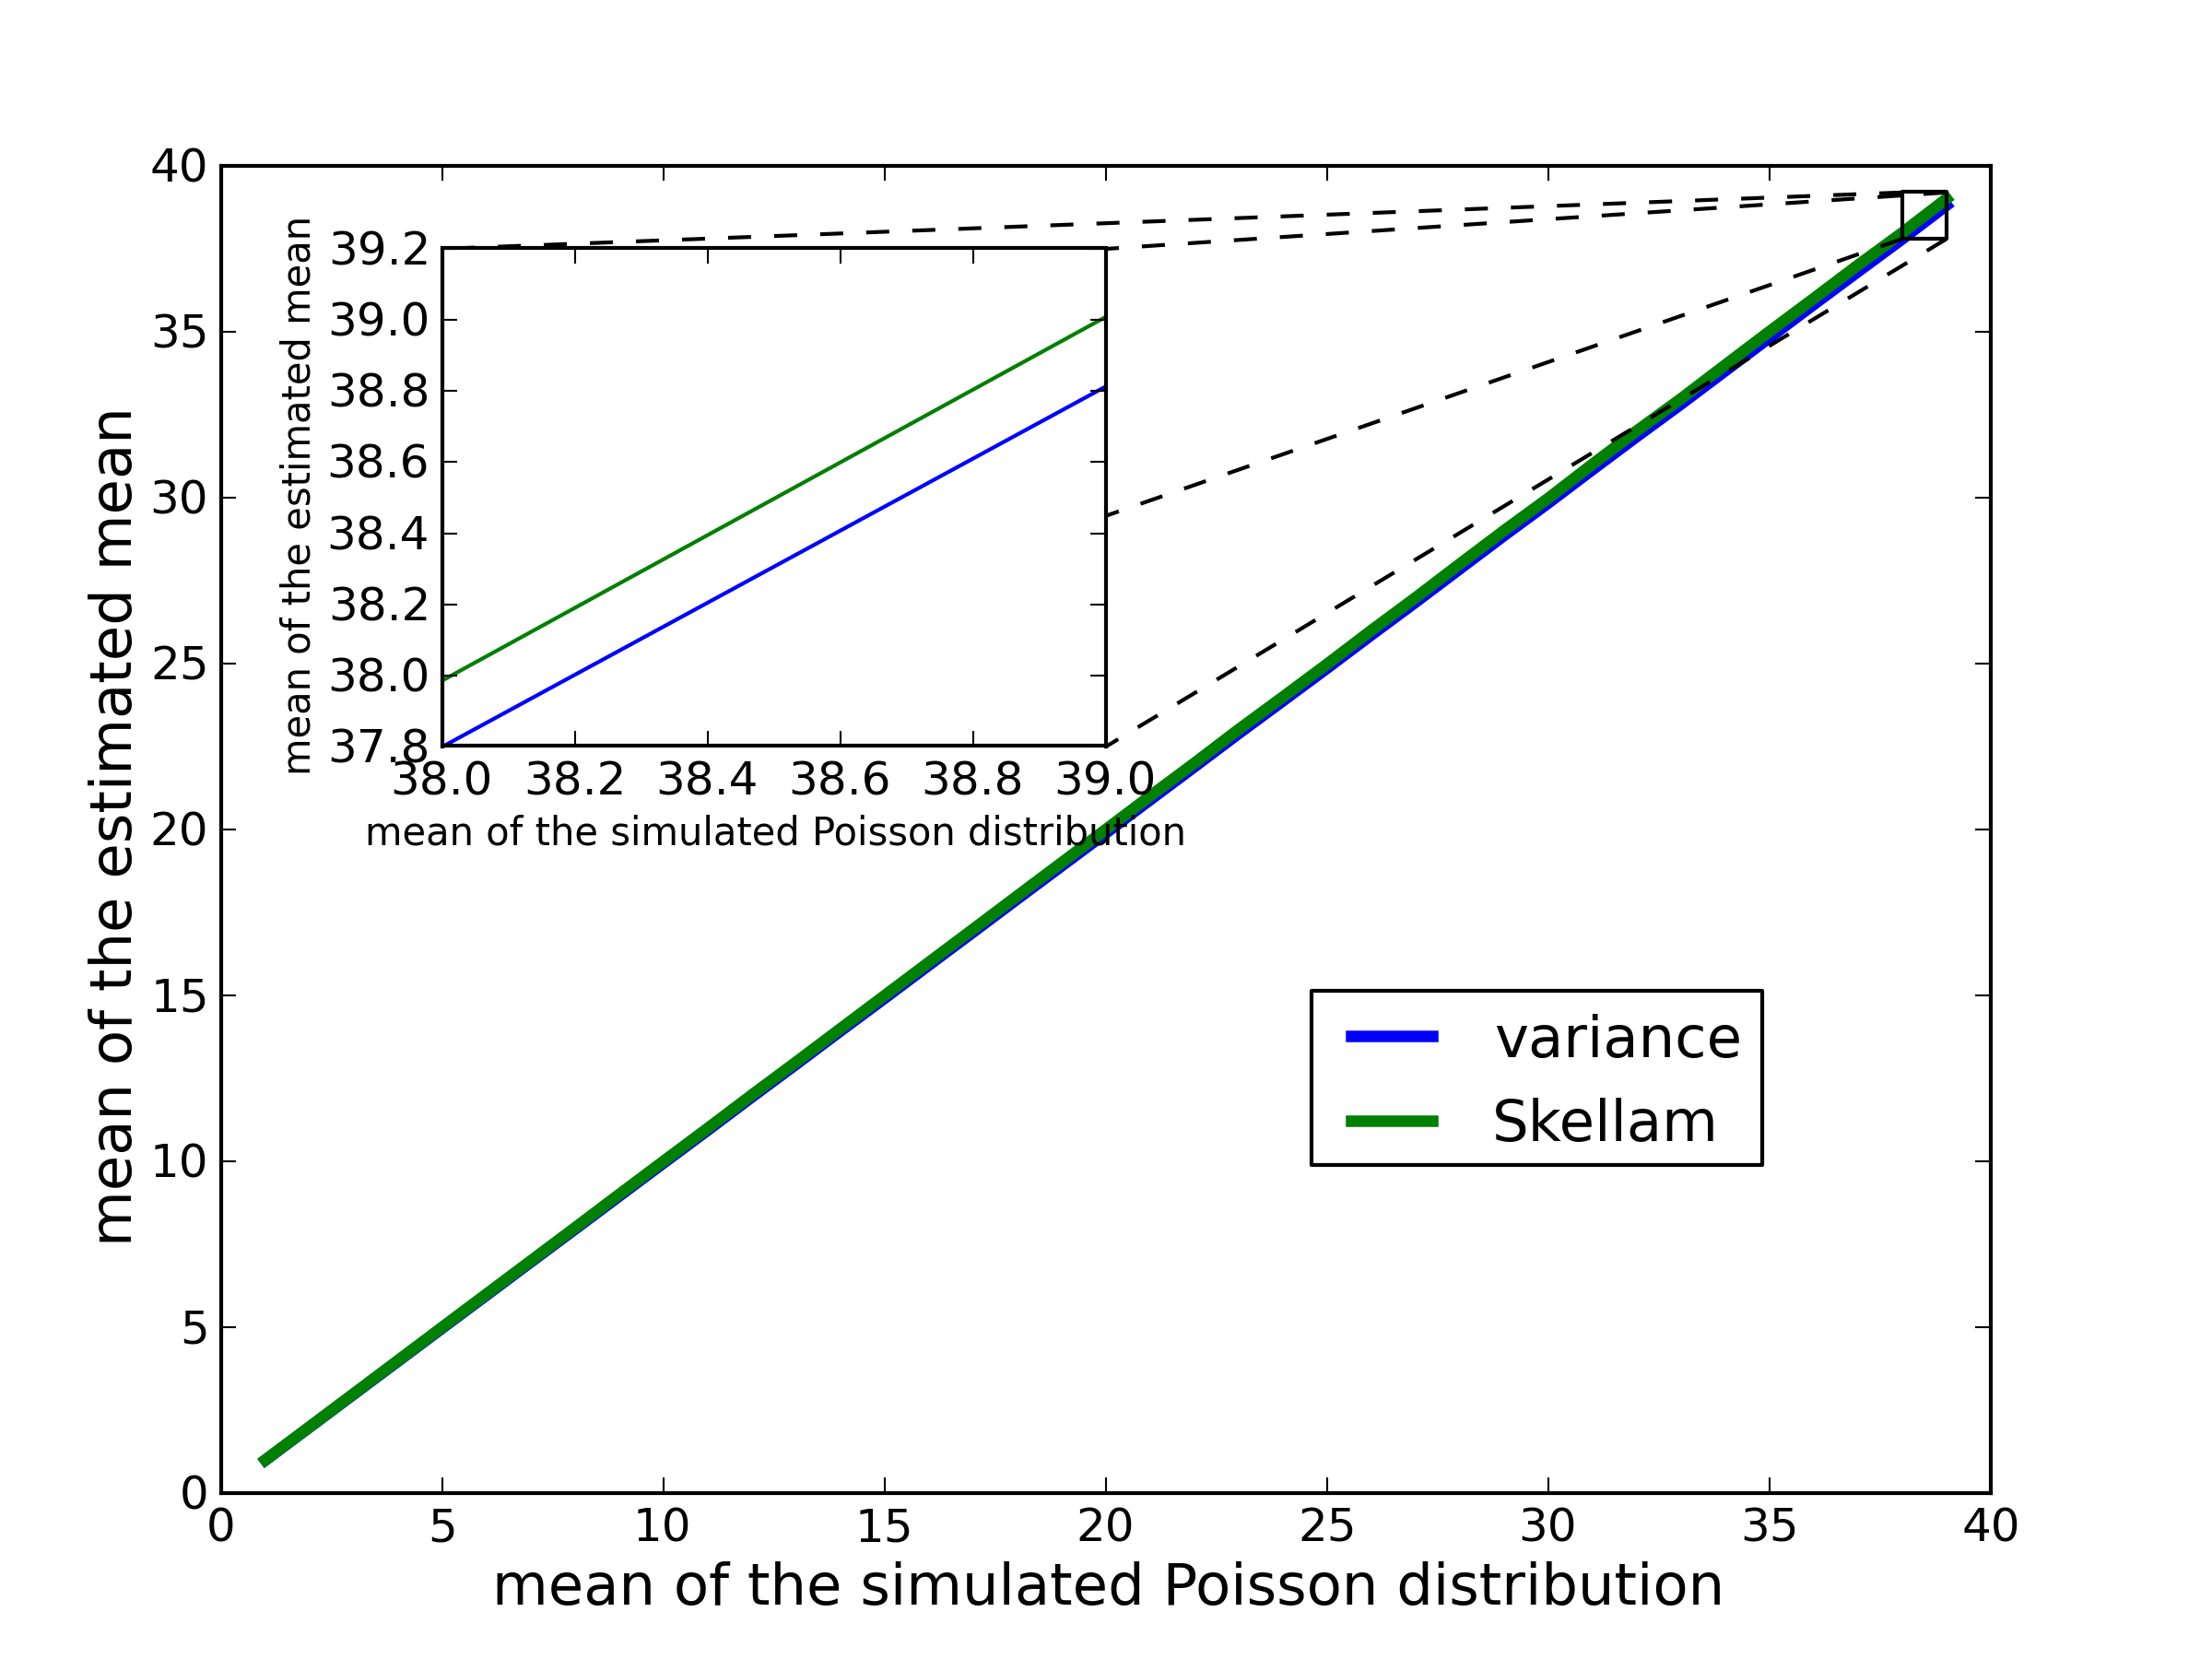
\includegraphics[width = \textwidth]{pictures/SkellamVarMean.png}
%\caption{Mean of the estimated variances.}\label{skellamvarmean}
%\end{minipage} \hfill
%\begin{minipage}{0.48\textwidth}
%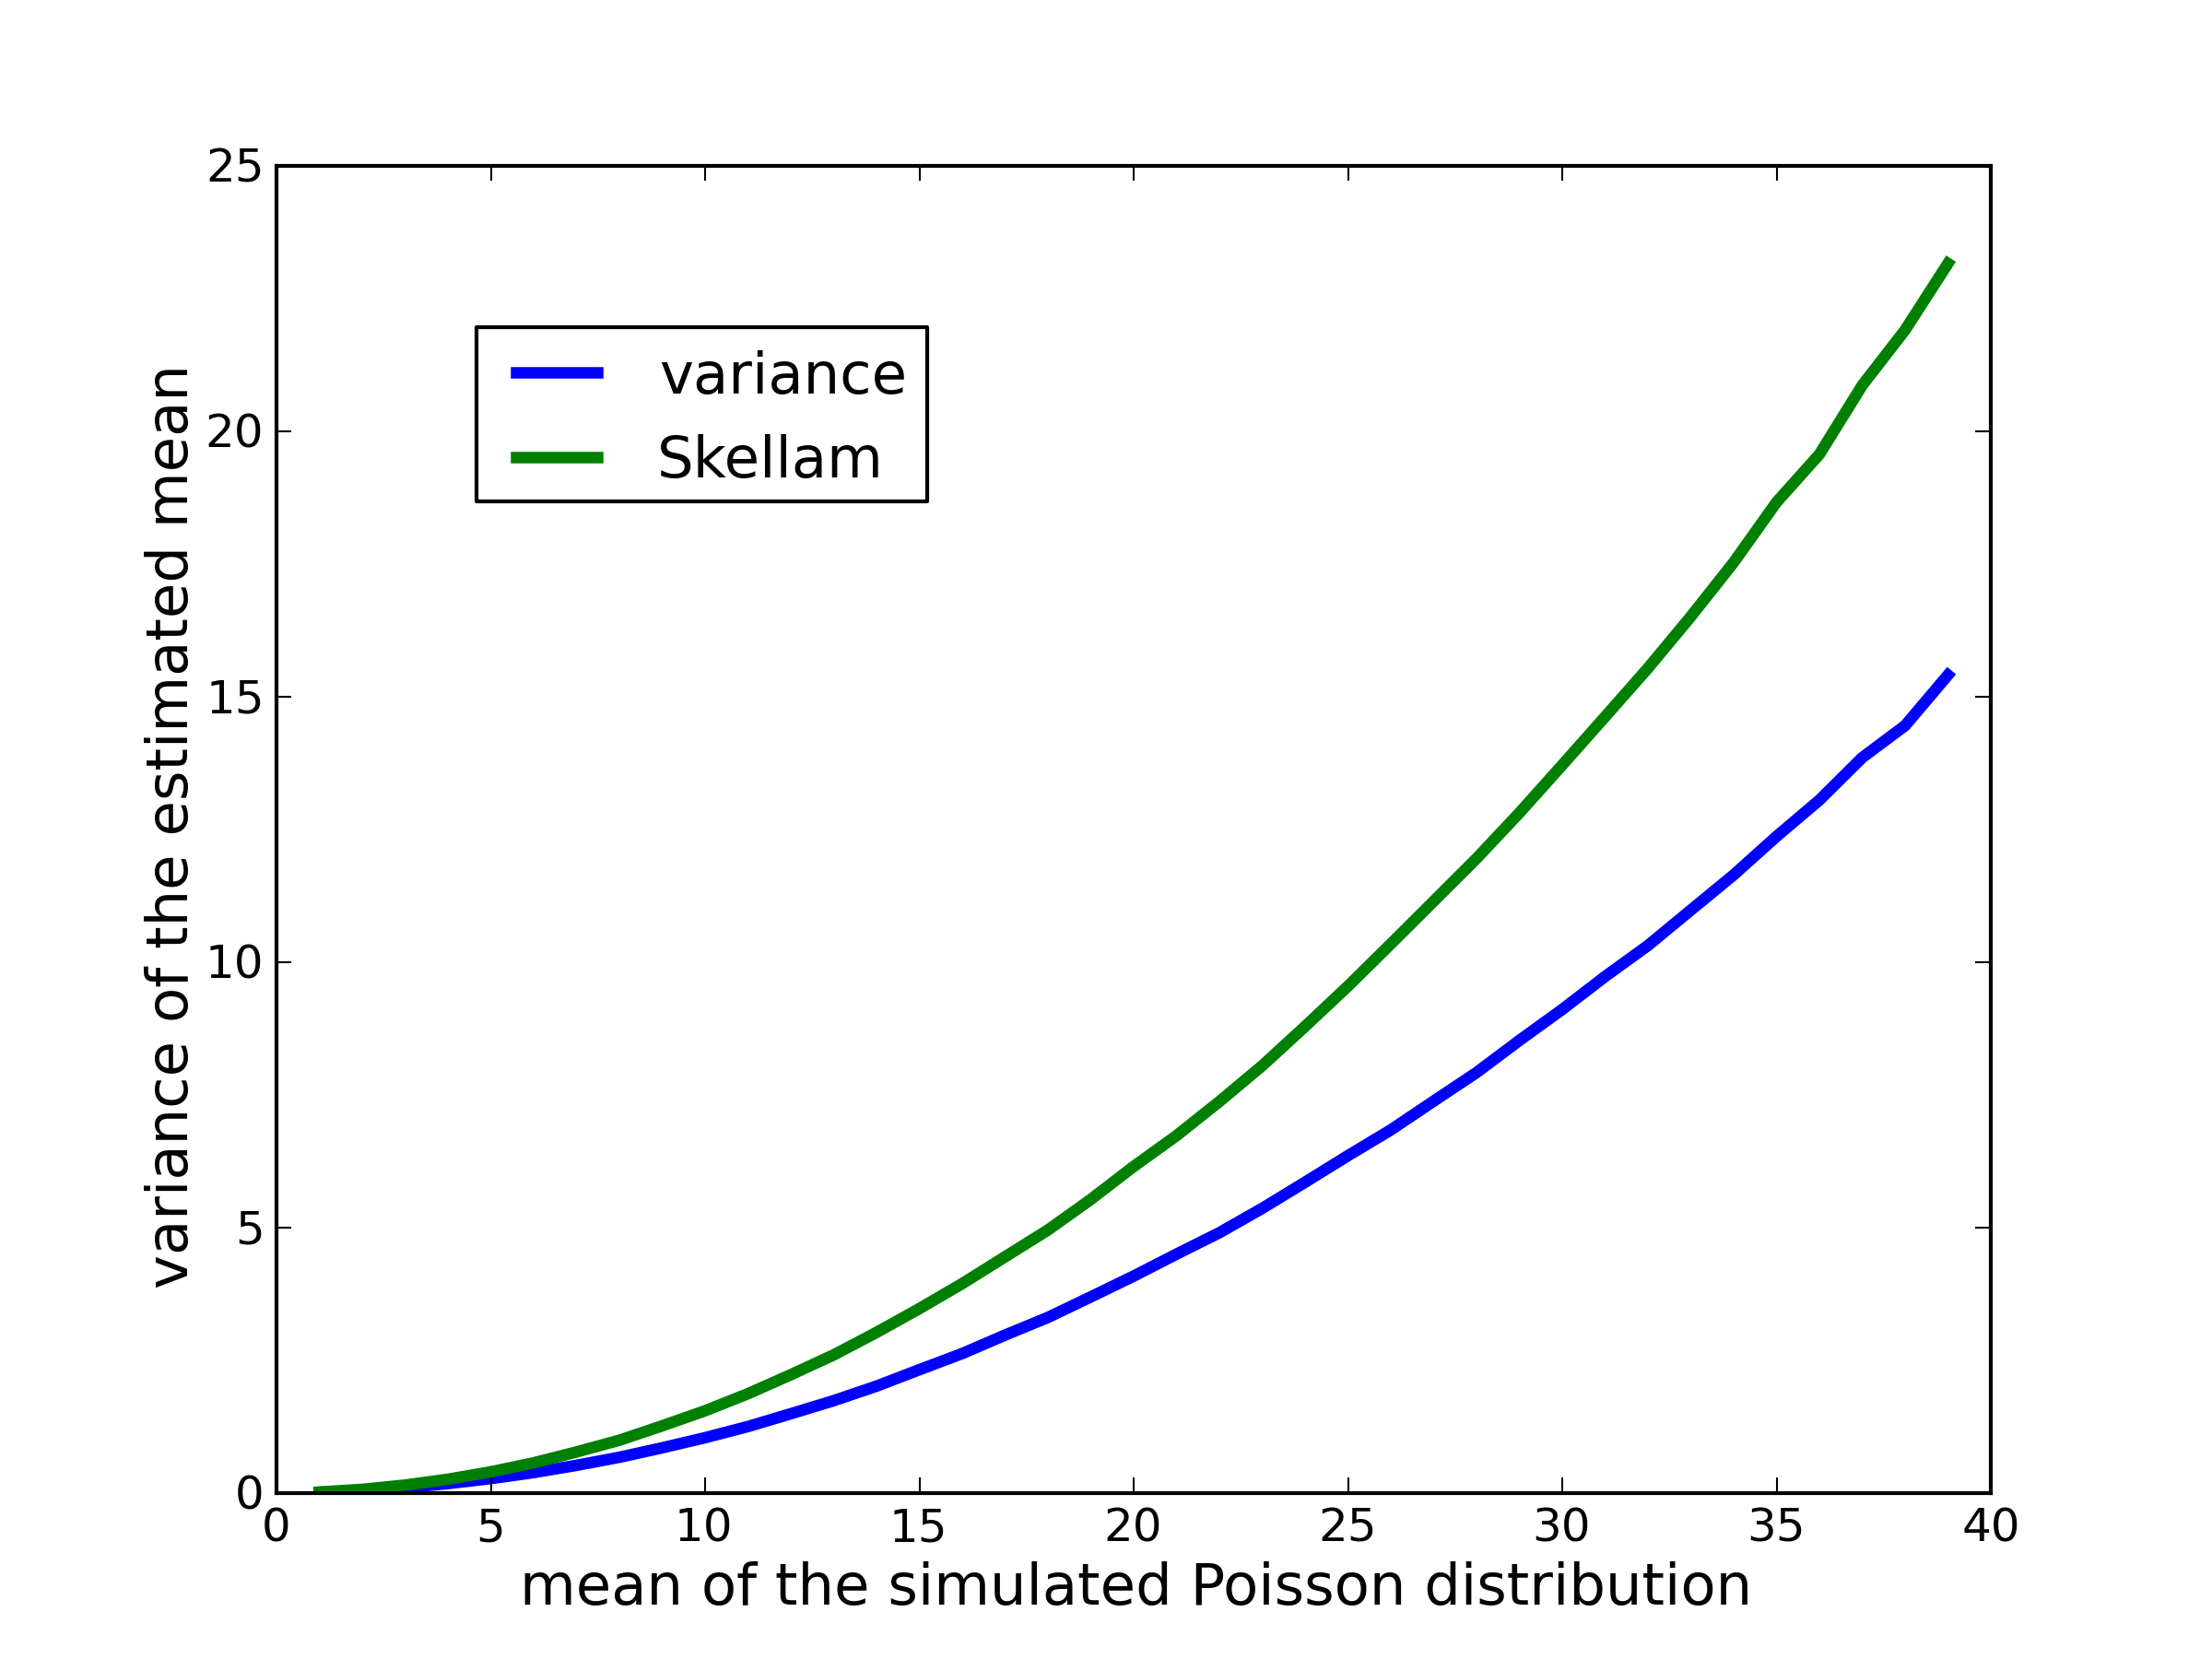
\includegraphics[width = \textwidth]{pictures/SkellamVarVar.png}
%\caption{Variance of the estimated variances.}\label{skellamvarvar}
%\end{minipage}
%\end{figure}
\begin{figure}
\centering
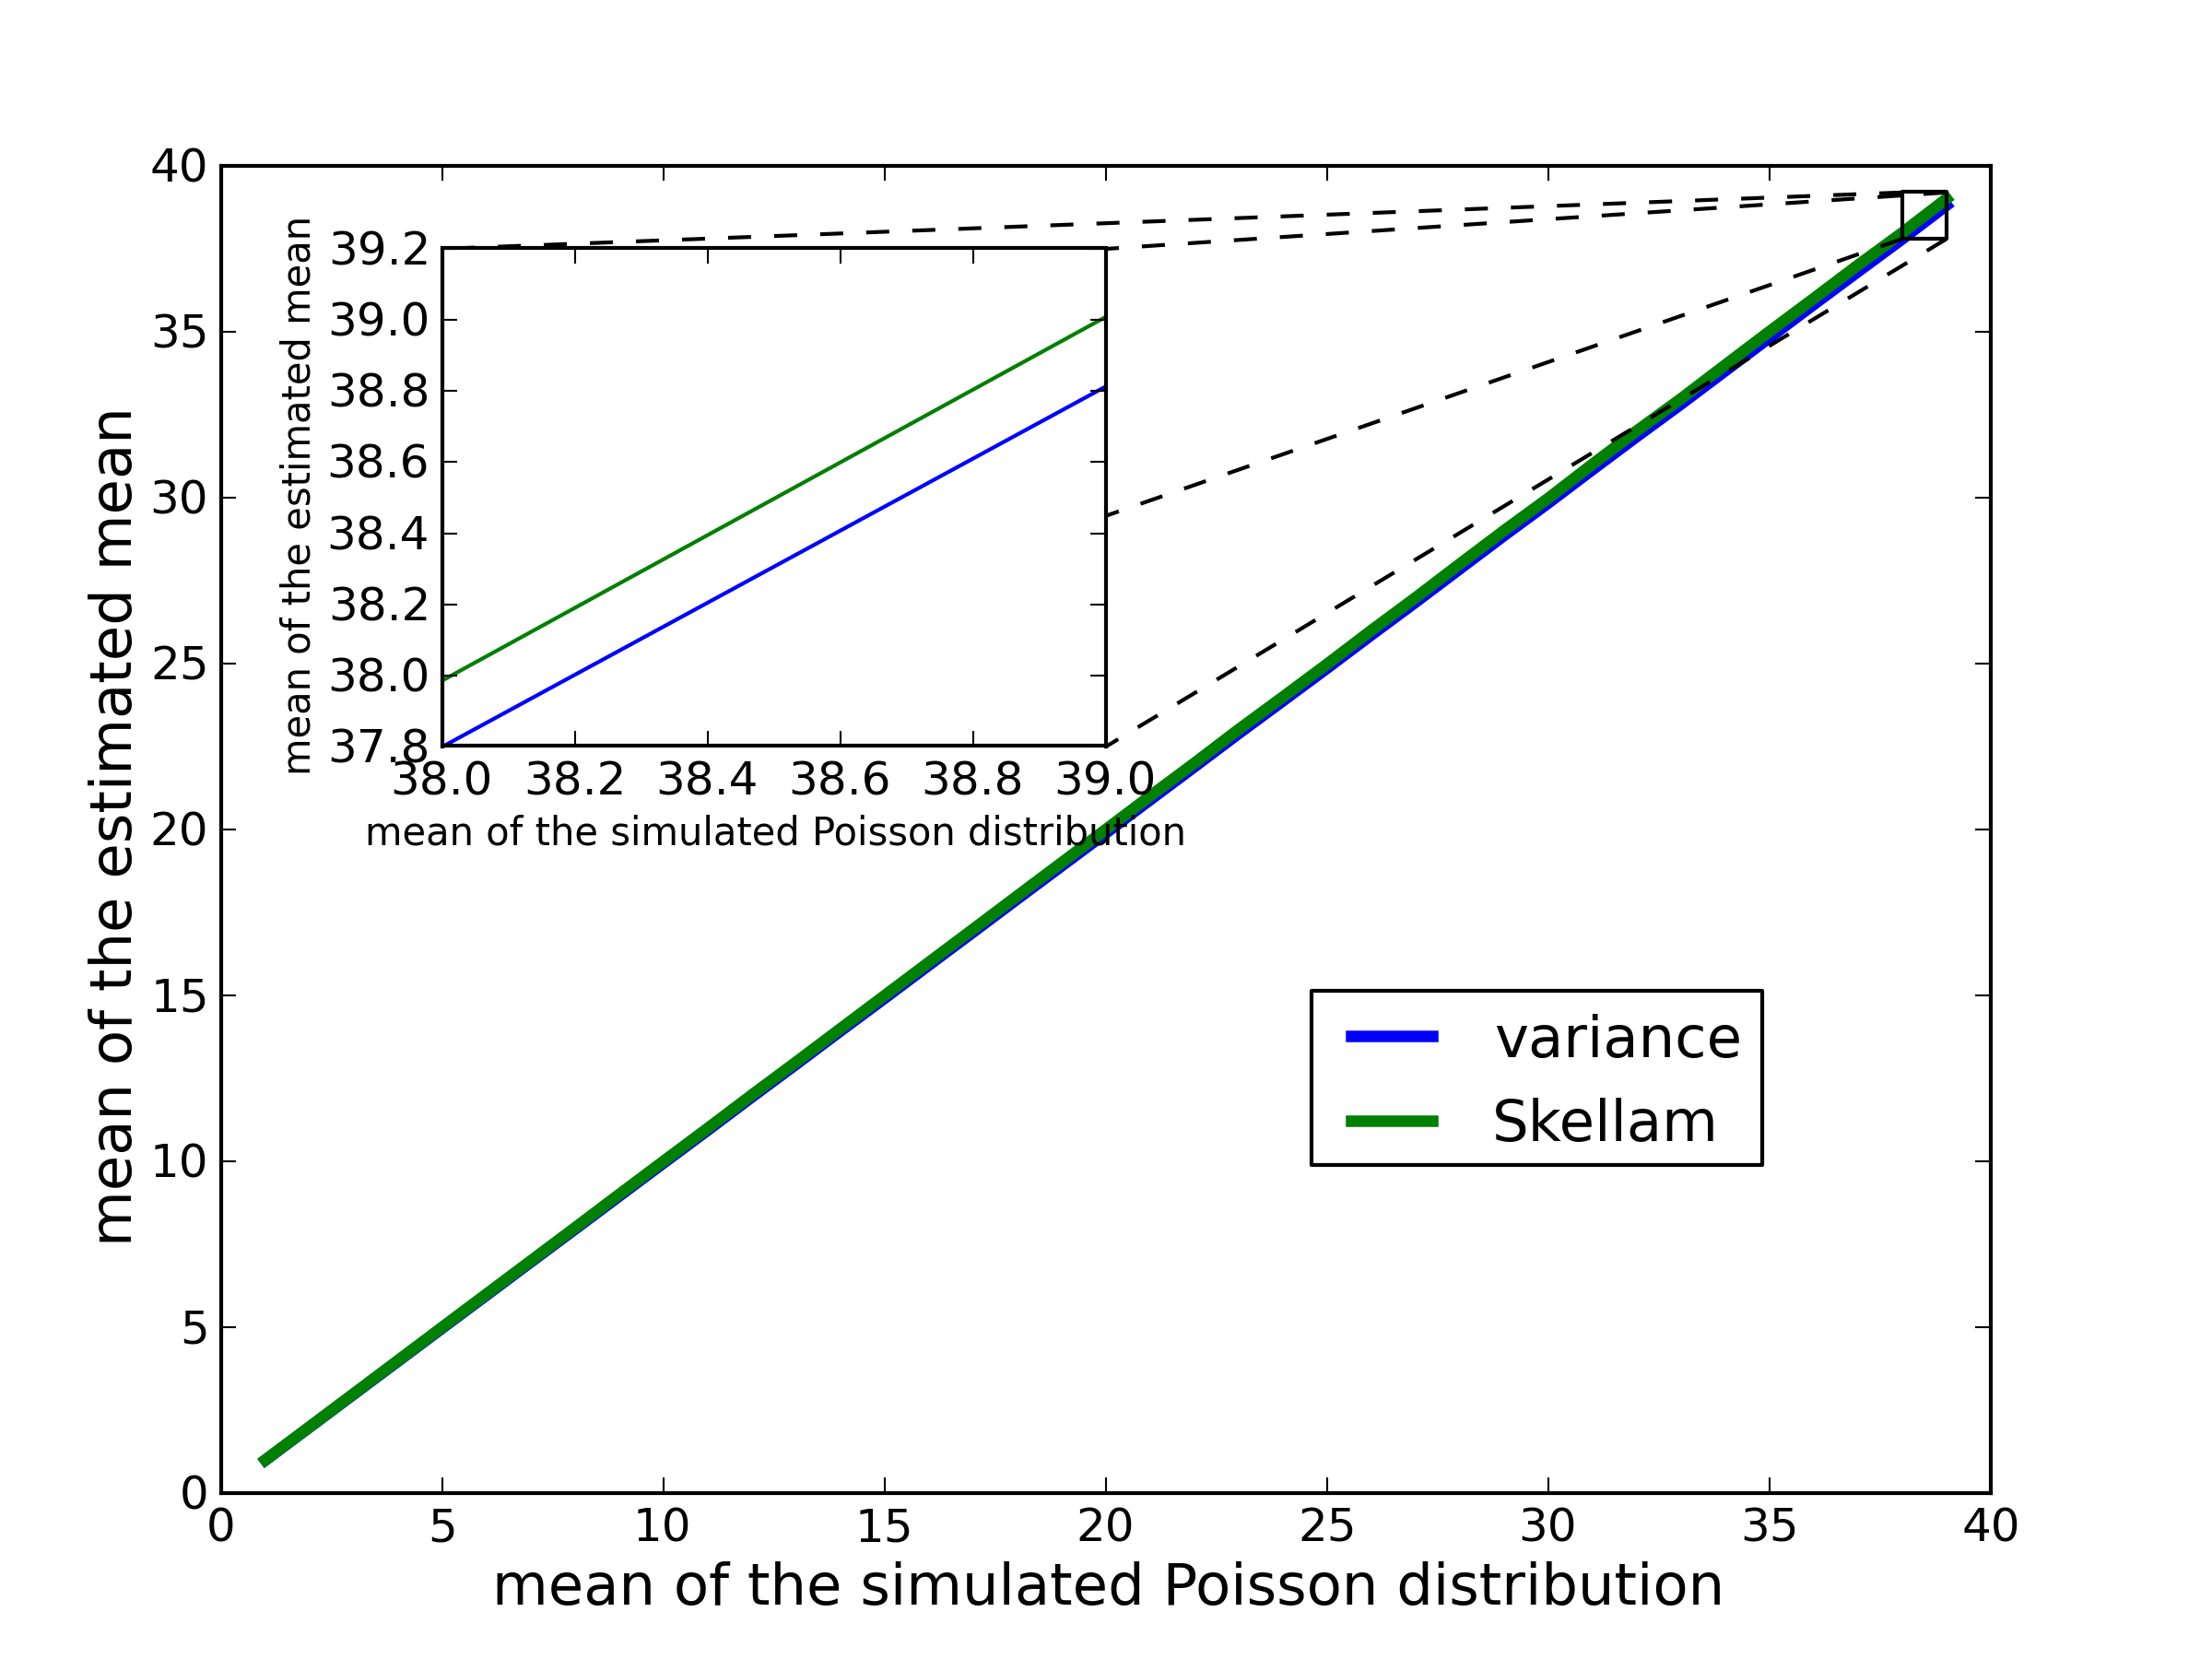
\includegraphics[width = .7\textwidth]{pictures/SkellamVarMean.png}
\caption{Mean of the estimated variances.}\label{skellamvarmean}
\end{figure}

\begin{figure}
\centering
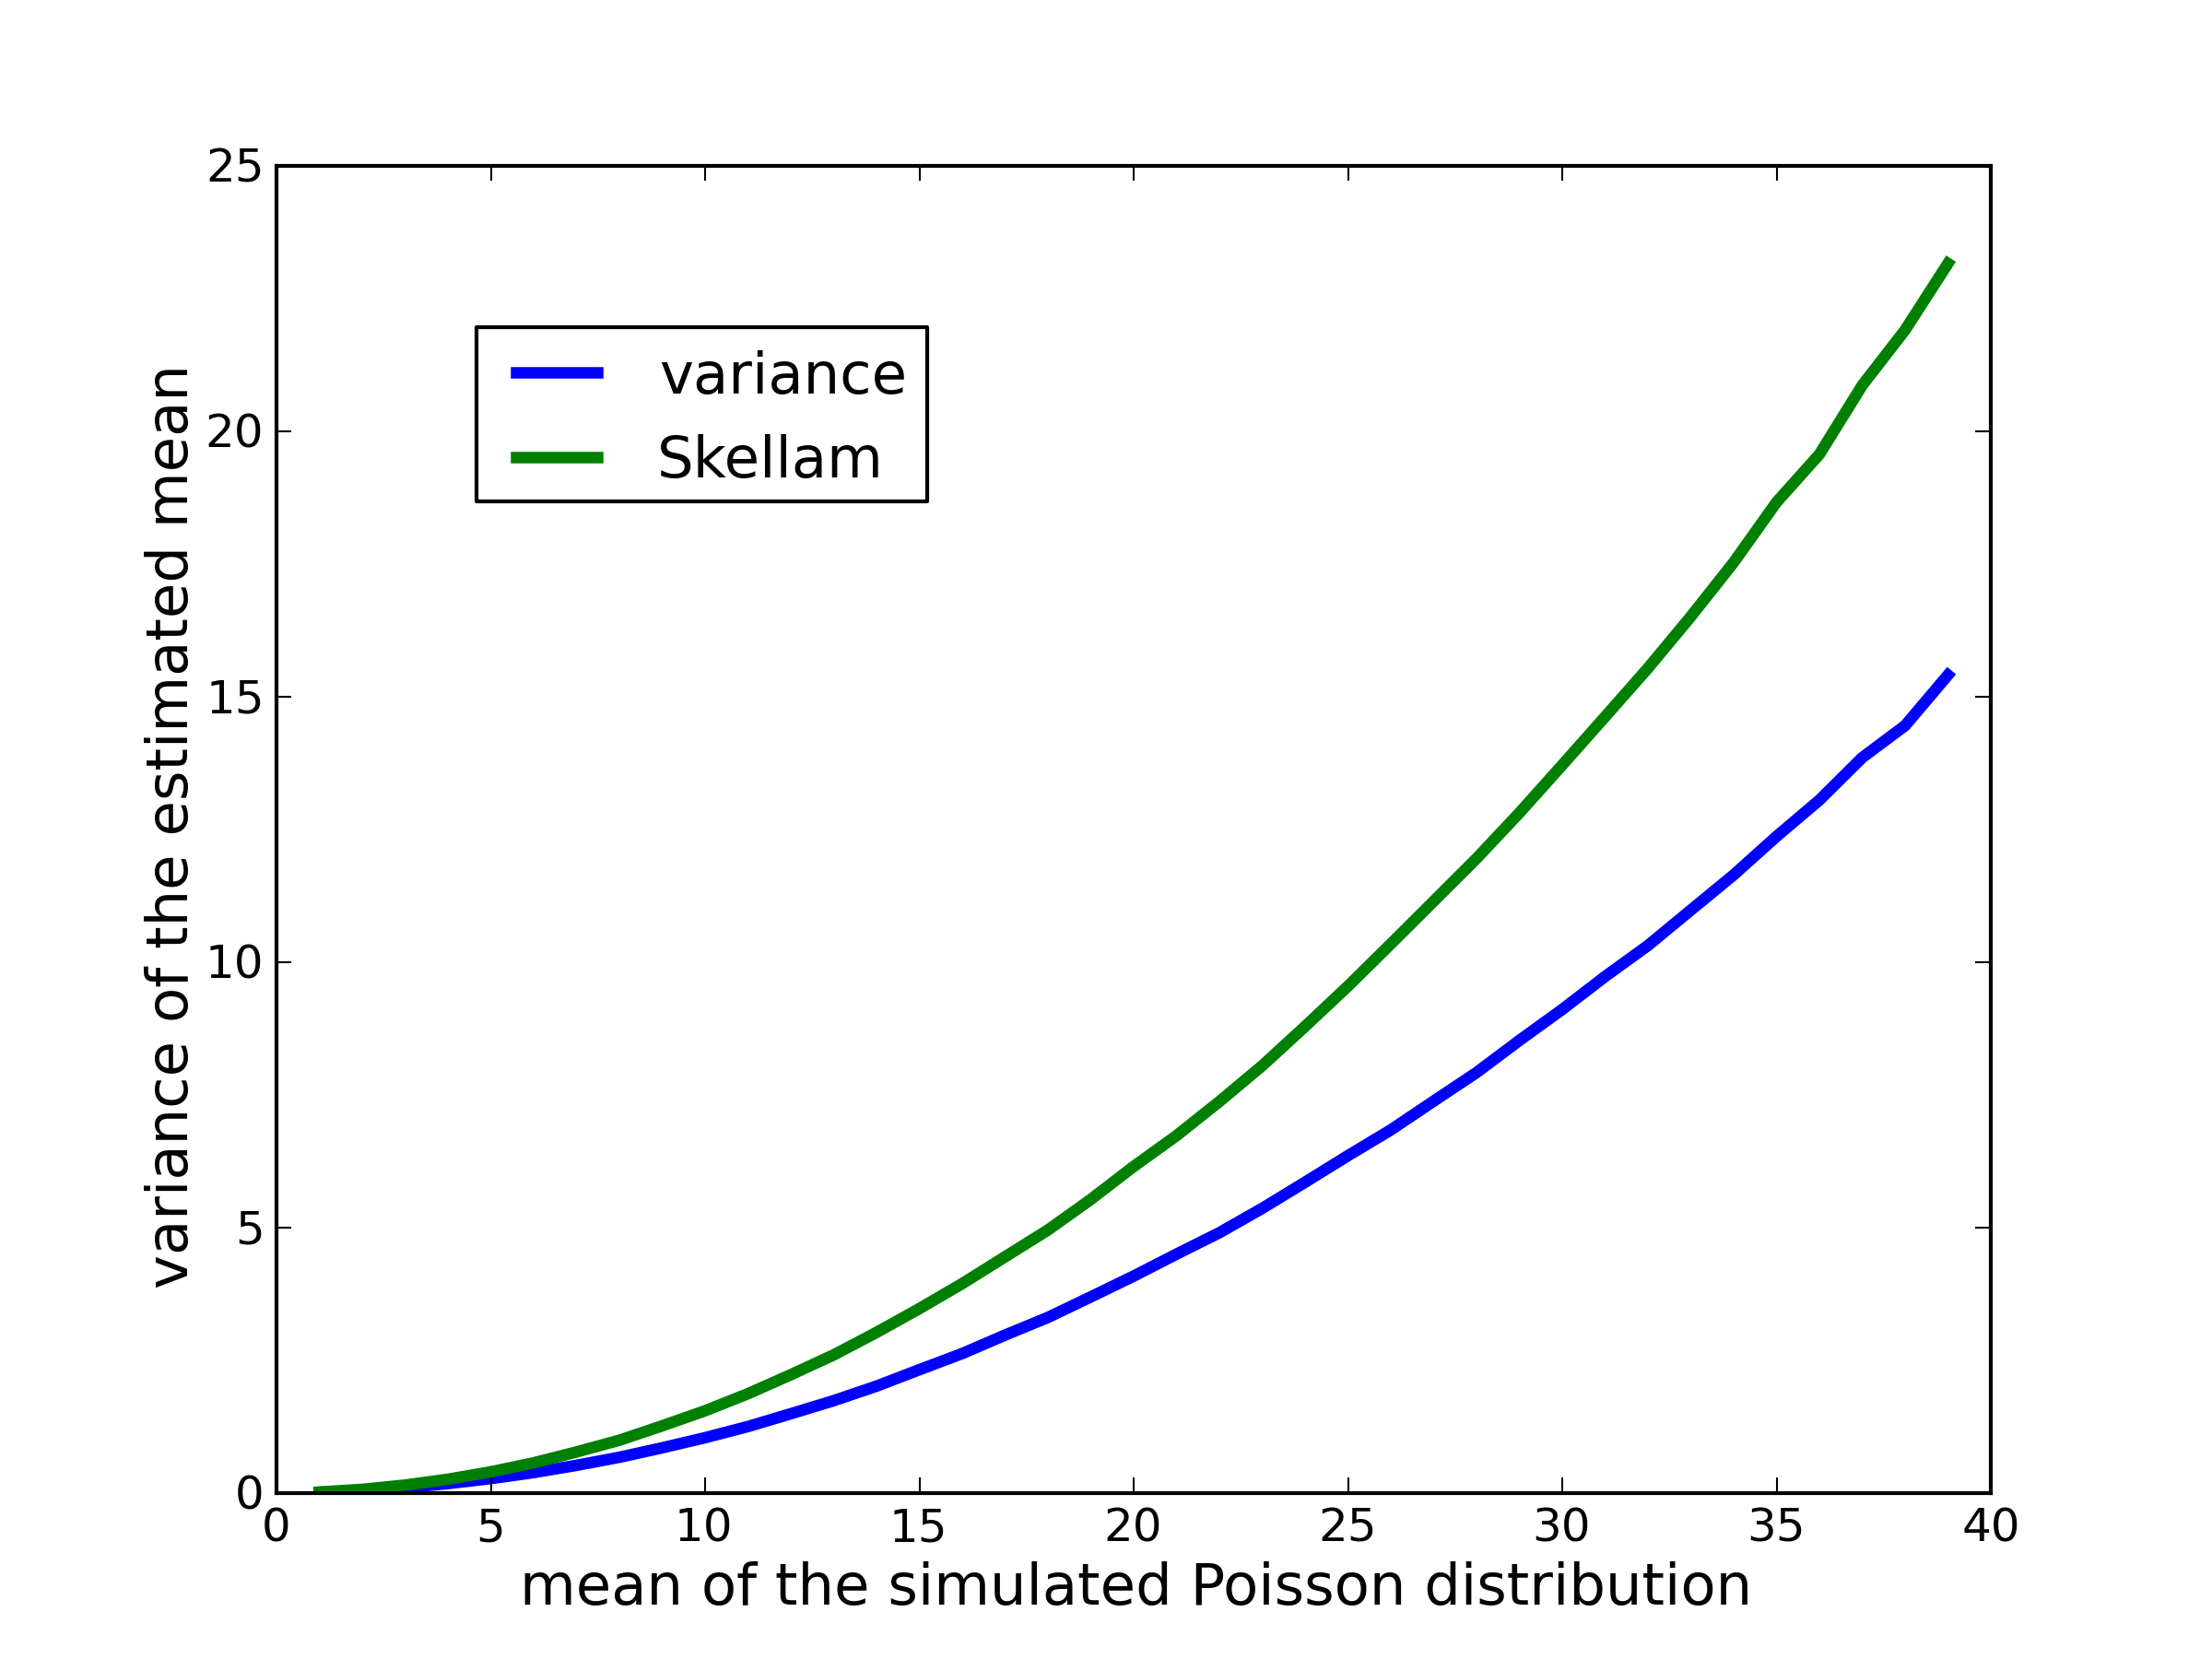
\includegraphics[width = .7\textwidth]{pictures/SkellamVarVar.png}
\caption{Variance of the estimated variances.}\label{skellamvarvar}
\end{figure}


\section{Best line fit method}
To get the correct gain and offset based on the mean intensities and the corresponding variances of the pixels intensities, a robust fitting method is needed. This is because of the phenomena described in section \ref{pointsabove}. In this section four different methods will be described and their performances compared.
\subsection{Different methods}
\subsubsection*{Based on minimum covariance determinant (Fit1)}
The base of this fitting approach is to find a compact subset of points that represent the inliers. To do so a R function based on the algorithm of \cite{ilia1} is used. For this algorithm many initial subsets of  the data are drawn. For each subset the of points the minimal covariance determinant is calculated. The subset with the smallest covariance determinant is taken. Weighted linear regression is performed on the selected subset of points. Therefore the $x$ range is split into several bins. For each bin the variance of the points is calculated and its inverse is used as weights for linear regression.
\subsubsection*{Use just lowest variances, weighted (Fit2)}
For each run half of the preselected points is chosen randomly. 
The mean values are splited into bins of equal witdth. Withing each bin the point with the lowest variance is found. Linear regression is performed on all this lowest points with the inverse variance of each bin as weights. 
\subsubsection*{Linear fit of a random number of points (Fit3)}
Bins are determined as above. From each bin just the lowest variance is considered. A linear fit is performed on a subset of this lowest points with varying size.
\subsubsection*{RANSAC (Fit4) and weighted RANSAC (Fit5)}\label{ransacdescr}
A standard RANSAC (random sample consensus) algorithm is used. Its pseudo code looks like this:
\begin{verbatim}
input:
    data - set of mean intensities and variances
    model - straight line 
    k - number iterations
    t - threshold for determining if a point fits the model
    d - number of close points that must be found at least not to discard the found model instantly
output:
    slope m and intercept c of the straight line

iteration = 0
best_m = 0
best_c = 0
best_error = inf
while iterations < k
    initial_guess_set = 2 random points from data
    m,c = fit_line(initial_guess_set)
    for every point in data
        if |y_point - m*x_point+c| < t
            add point to consensus_set
    m,c,current_error = fit_line(consensus_set)
    if len(consensus_set)>d and current_error < best_error
        best_error = current_error
        best_m = m
        best_c = c

return best_m, best_c
\end{verbatim}
For the weighted RANSAC instead of a linear fit, a weighted line fit is done. The weights are determined as for the other weighted fitting methods.
\subsubsection*{Simple fit (Fit6)}
For this very simple approach, a certain number of points is chosen randomly from all points. A straight line is fitted and the mean square error for the current set of points is computed. This is done several times. The best fit with the lowest mean square error is taken as the final result.

\subsection{Discussion} 
The goal is to find a robust fitting method. Figures \ref{lineplot1} and \ref{lineplot2} show scatter plots of the means and variances of the preselected points and the results of the fits.
It is difficult to determine the best fit by looking at the results, because there is not only one line but two or more visible.
The calibration measurement yields a gain factor of 3.9 and a offset off 380. Table \ref{tablefits} shows the fit results for offset and gain. The results from the weighted RANSAC method (Fit 5) are closest to the results from the calibration measurement. This table also illustrates why for the offset the minimal value is used instead of the estimated value.\newline
For the parameter estimation the weighted RANSAC method is used.


\begin{footnotesize}
\begin{center}
%\caption{Results for the main submission (with postprocessing)}
\captionof{table}{Fitting results for gain and offset for various data sets from our collaborators from Bioquant.}\label{tablefits}%
\begin{tabular}{l||c|c||c|c||c|c||c|c||c|c||c|c||}
Data set&\multicolumn{2}{c||}{Fit 1}&\multicolumn{2}{c||}{Fit 2}&\multicolumn{2}{c||}{Fit 3}&\multicolumn{2}{c||}{Fit 4}&\multicolumn{2}{c||}{Fit 5}&\multicolumn{2}{c||}{Fit 6}\\
&$g$&$o$&$g$&$o$&$g$&$o$&$g$&$o$&$g$&$o$&$g$&$o$\\\hline
110215\_HeLa1\_Er647&21.4&435&16.6&430&20.0&474&2.37&282&4.17&350&8.37&402\\\hline
110302\_ER-Alexa647&12.3&458&19.1&432&11.3&479&4.42&358&4.42&358&8.00&410\\\hline
110302\_HeLa1\_ER647&7.56&437&6.45&452&6.68&474&3.22&228&2.69&156&4.21&269\\\hline
Pos2\_2\_green&12.6&484&7.05&452&7.12&483&3.13&308&3.44&329&5.76&407\\\hline
Pos2\_2\_red&6.67&378&7.26&443&7.78&474&3.82&374&4.31&380&6.18&396\\\hline
Pos11\_2\_green&12.9&442&8.17&395&9.15&474&4.51&376&4.59&378&5.83&390\\\hline
Pos11\_2\_red&11.0&390&20.3&839&10.6&443&3.78&359&3.84&361&9.89&416\\\hline
Tetra1\_high\_568&5.33&387&4.74&394&3.97&387&4.11&379&4.12&380&4.68&382
\end{tabular} 

\end{center}
\end{footnotesize}
 
\begin{figure}
\subfloat[110215\_HeLa1\_Er647]{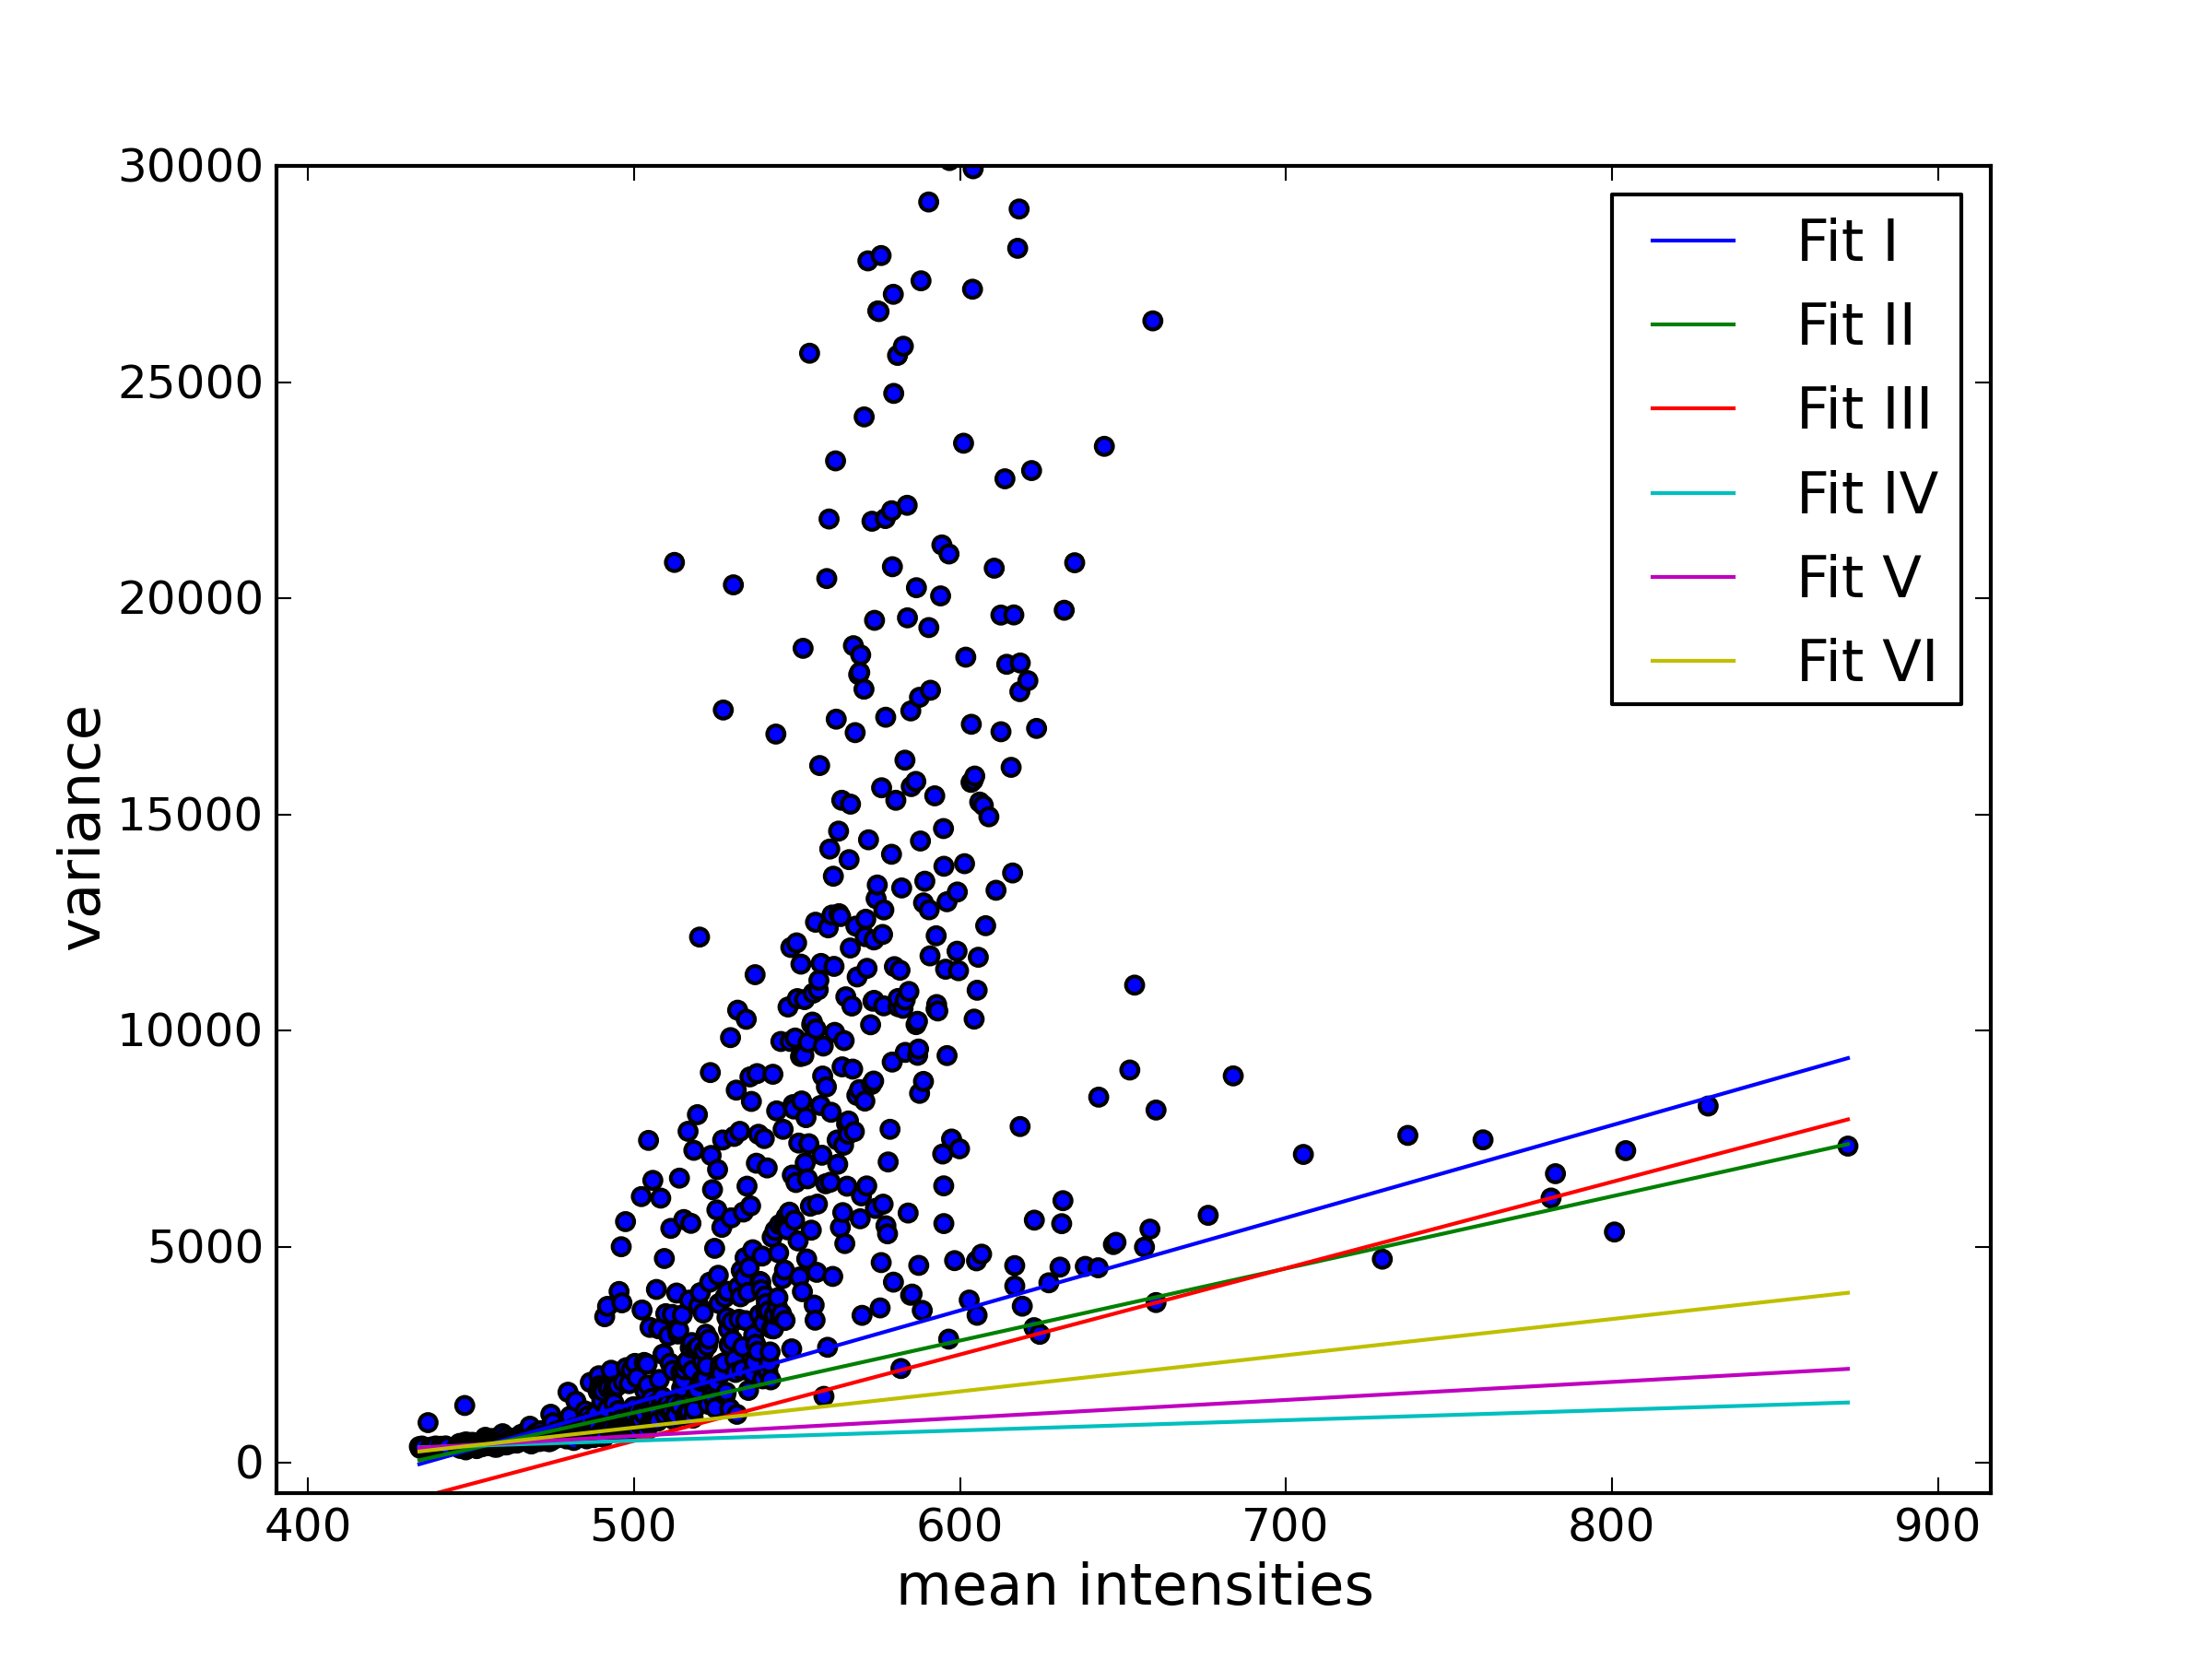
\includegraphics[width =0.48\textwidth]{pictures/geradenplots/110215hela.png}}\hfill
\subfloat[110302\_ER-Alexa647]{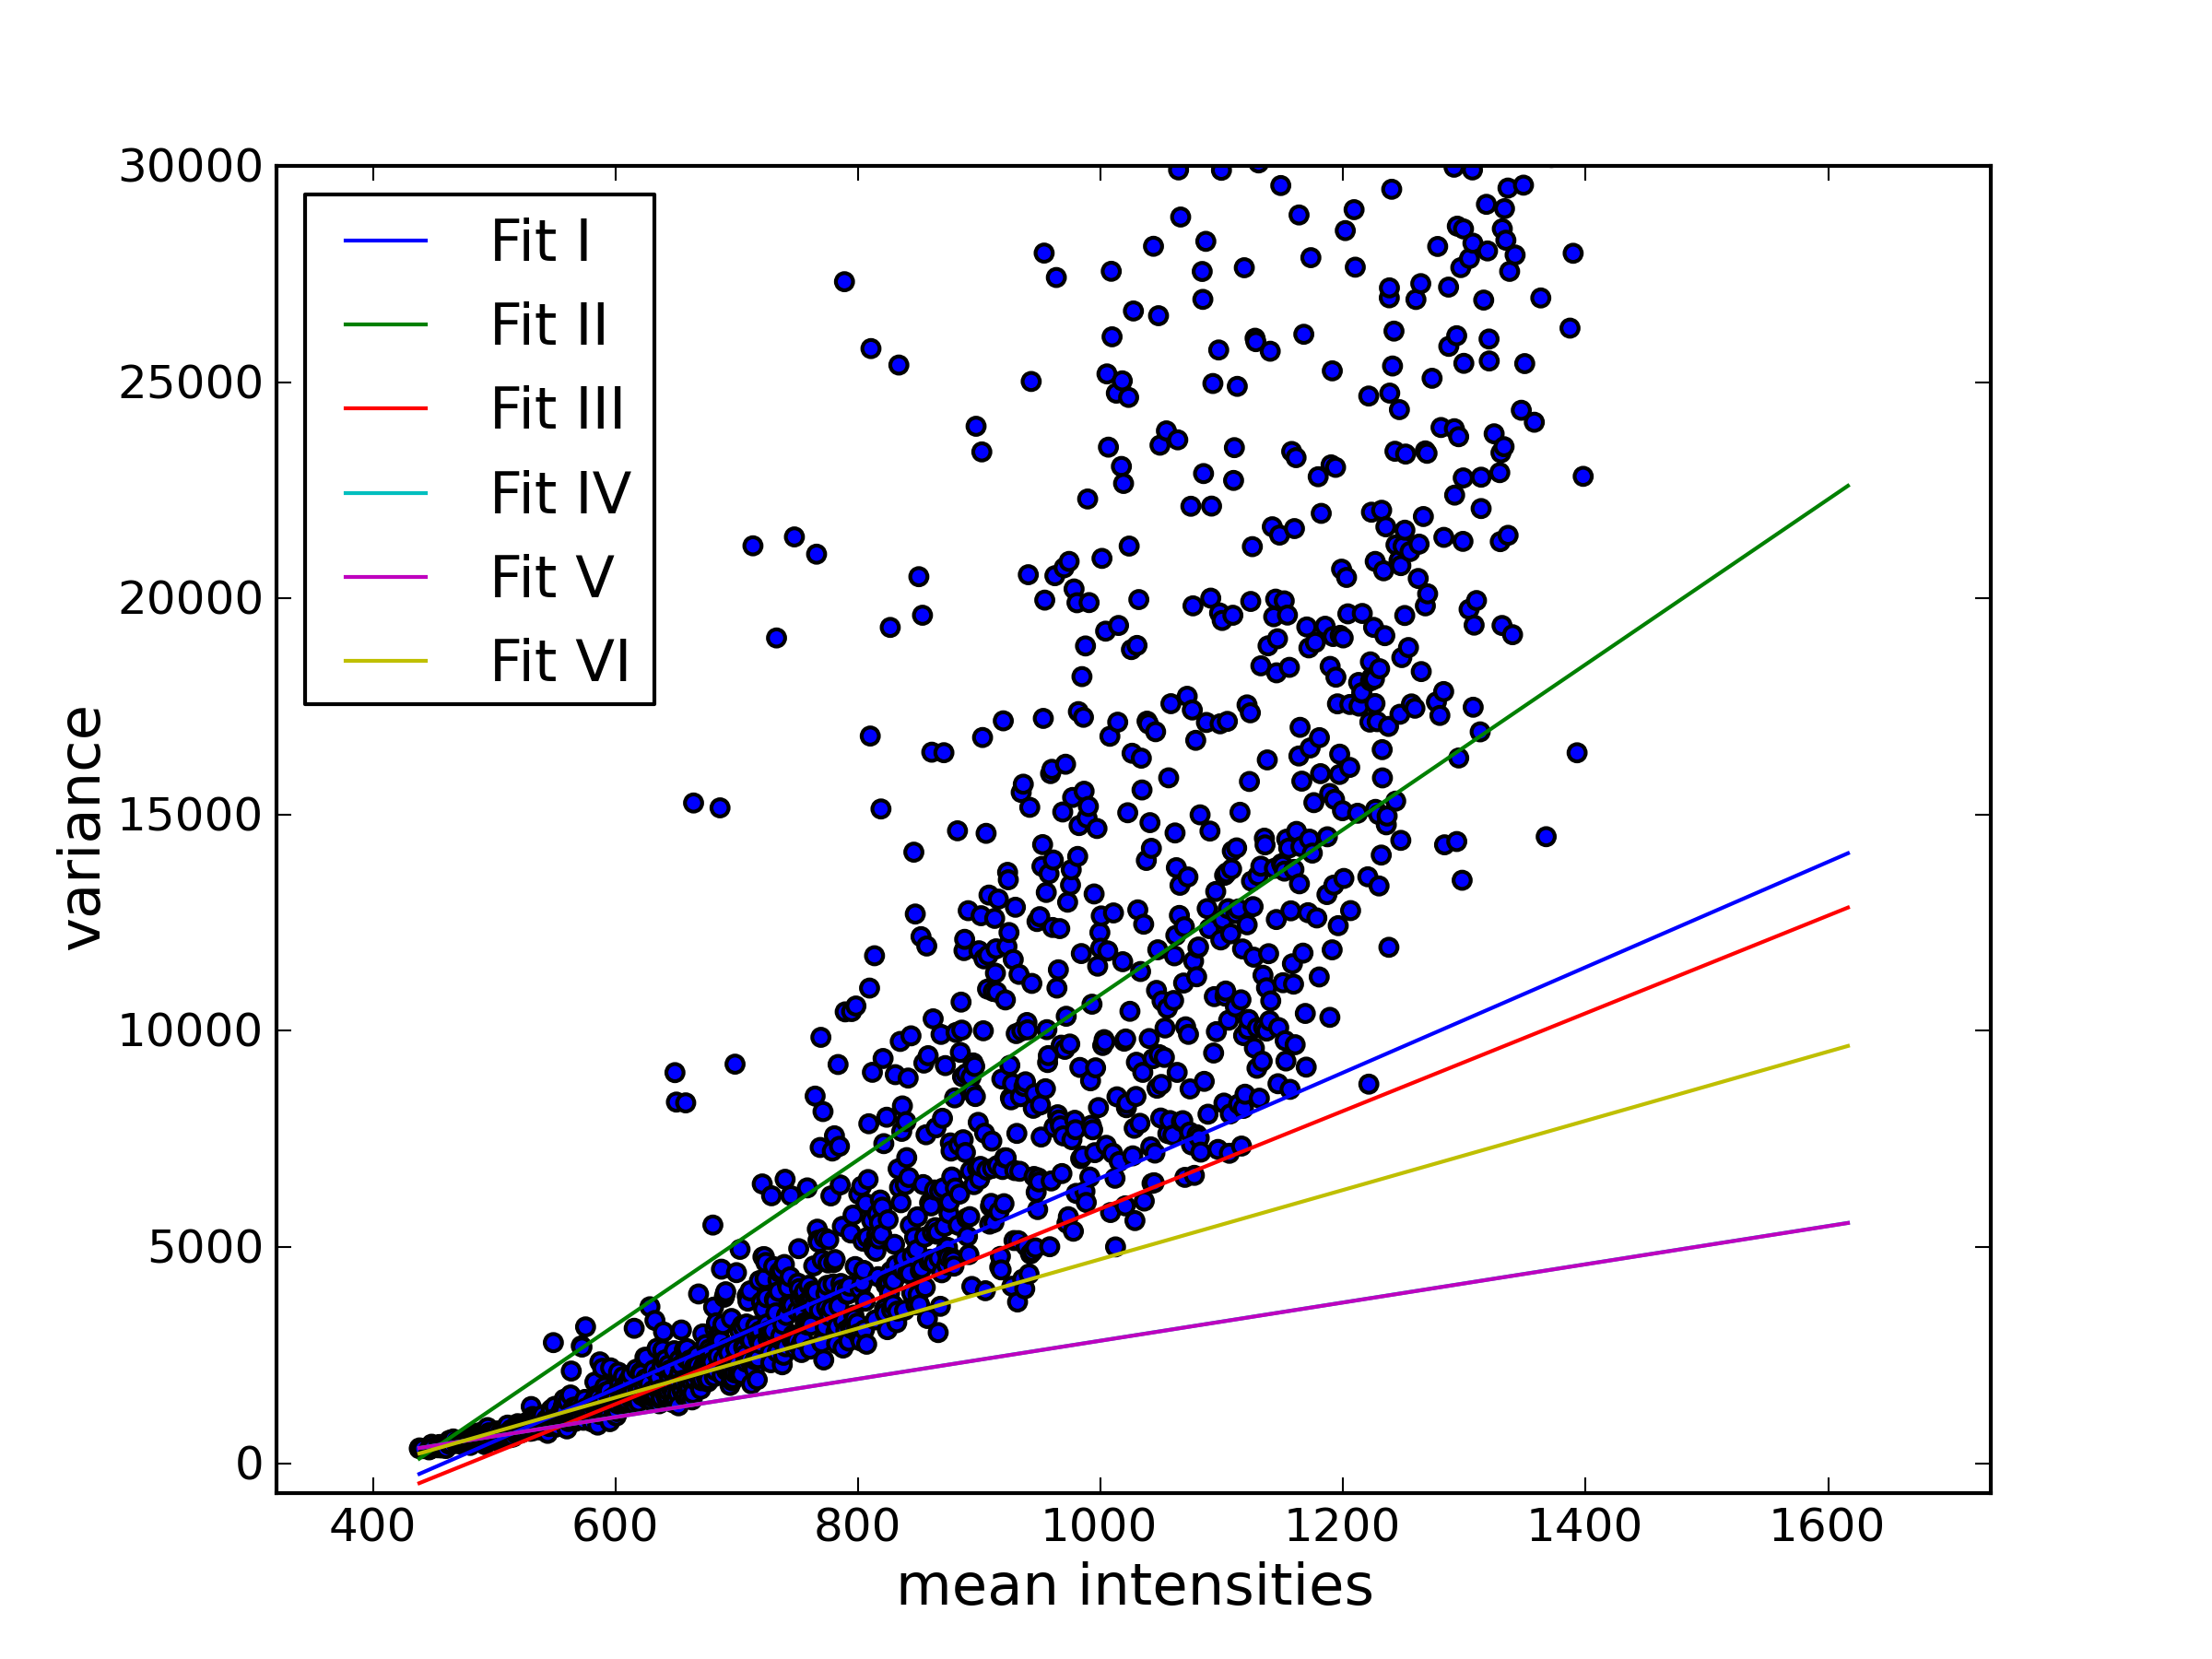
\includegraphics[width =0.48\textwidth]{pictures/geradenplots/110302alexa647.png}}\\
\subfloat[110302\_HeLa1\_ER647]{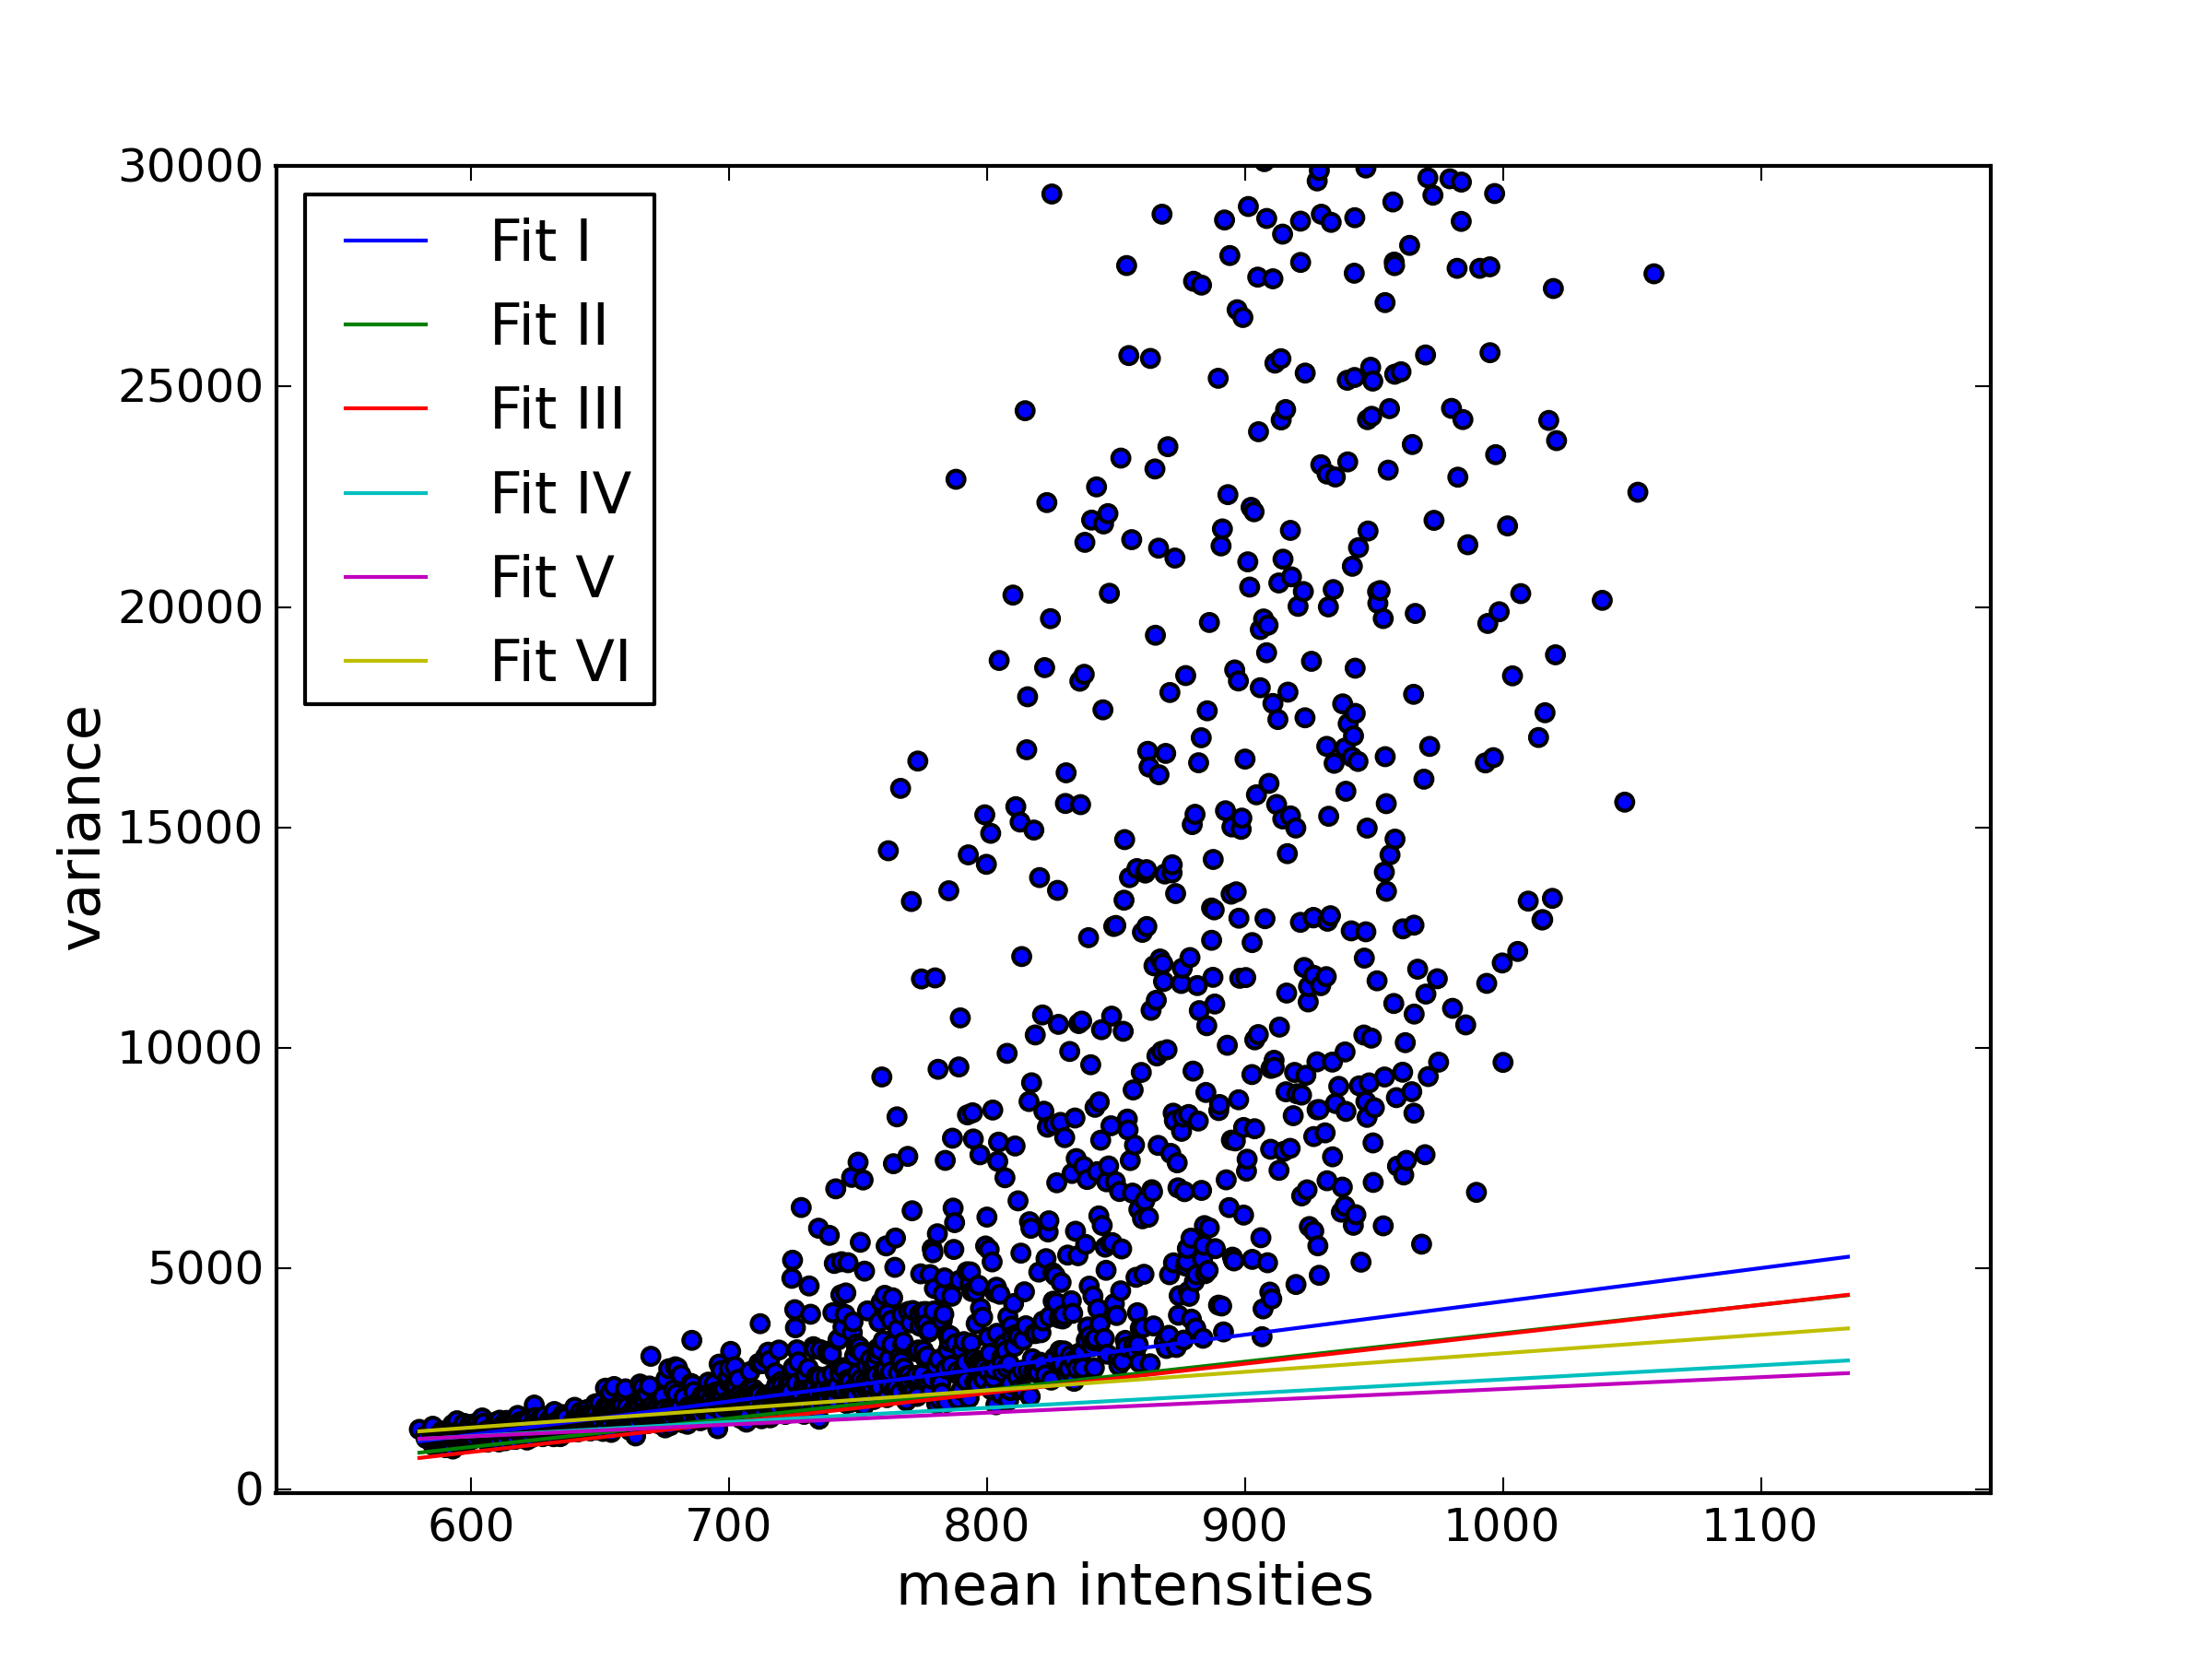
\includegraphics[width =0.48\textwidth]{pictures/geradenplots/110302hela647.png}}\hfill
\subfloat[Pos2\_2\_green]{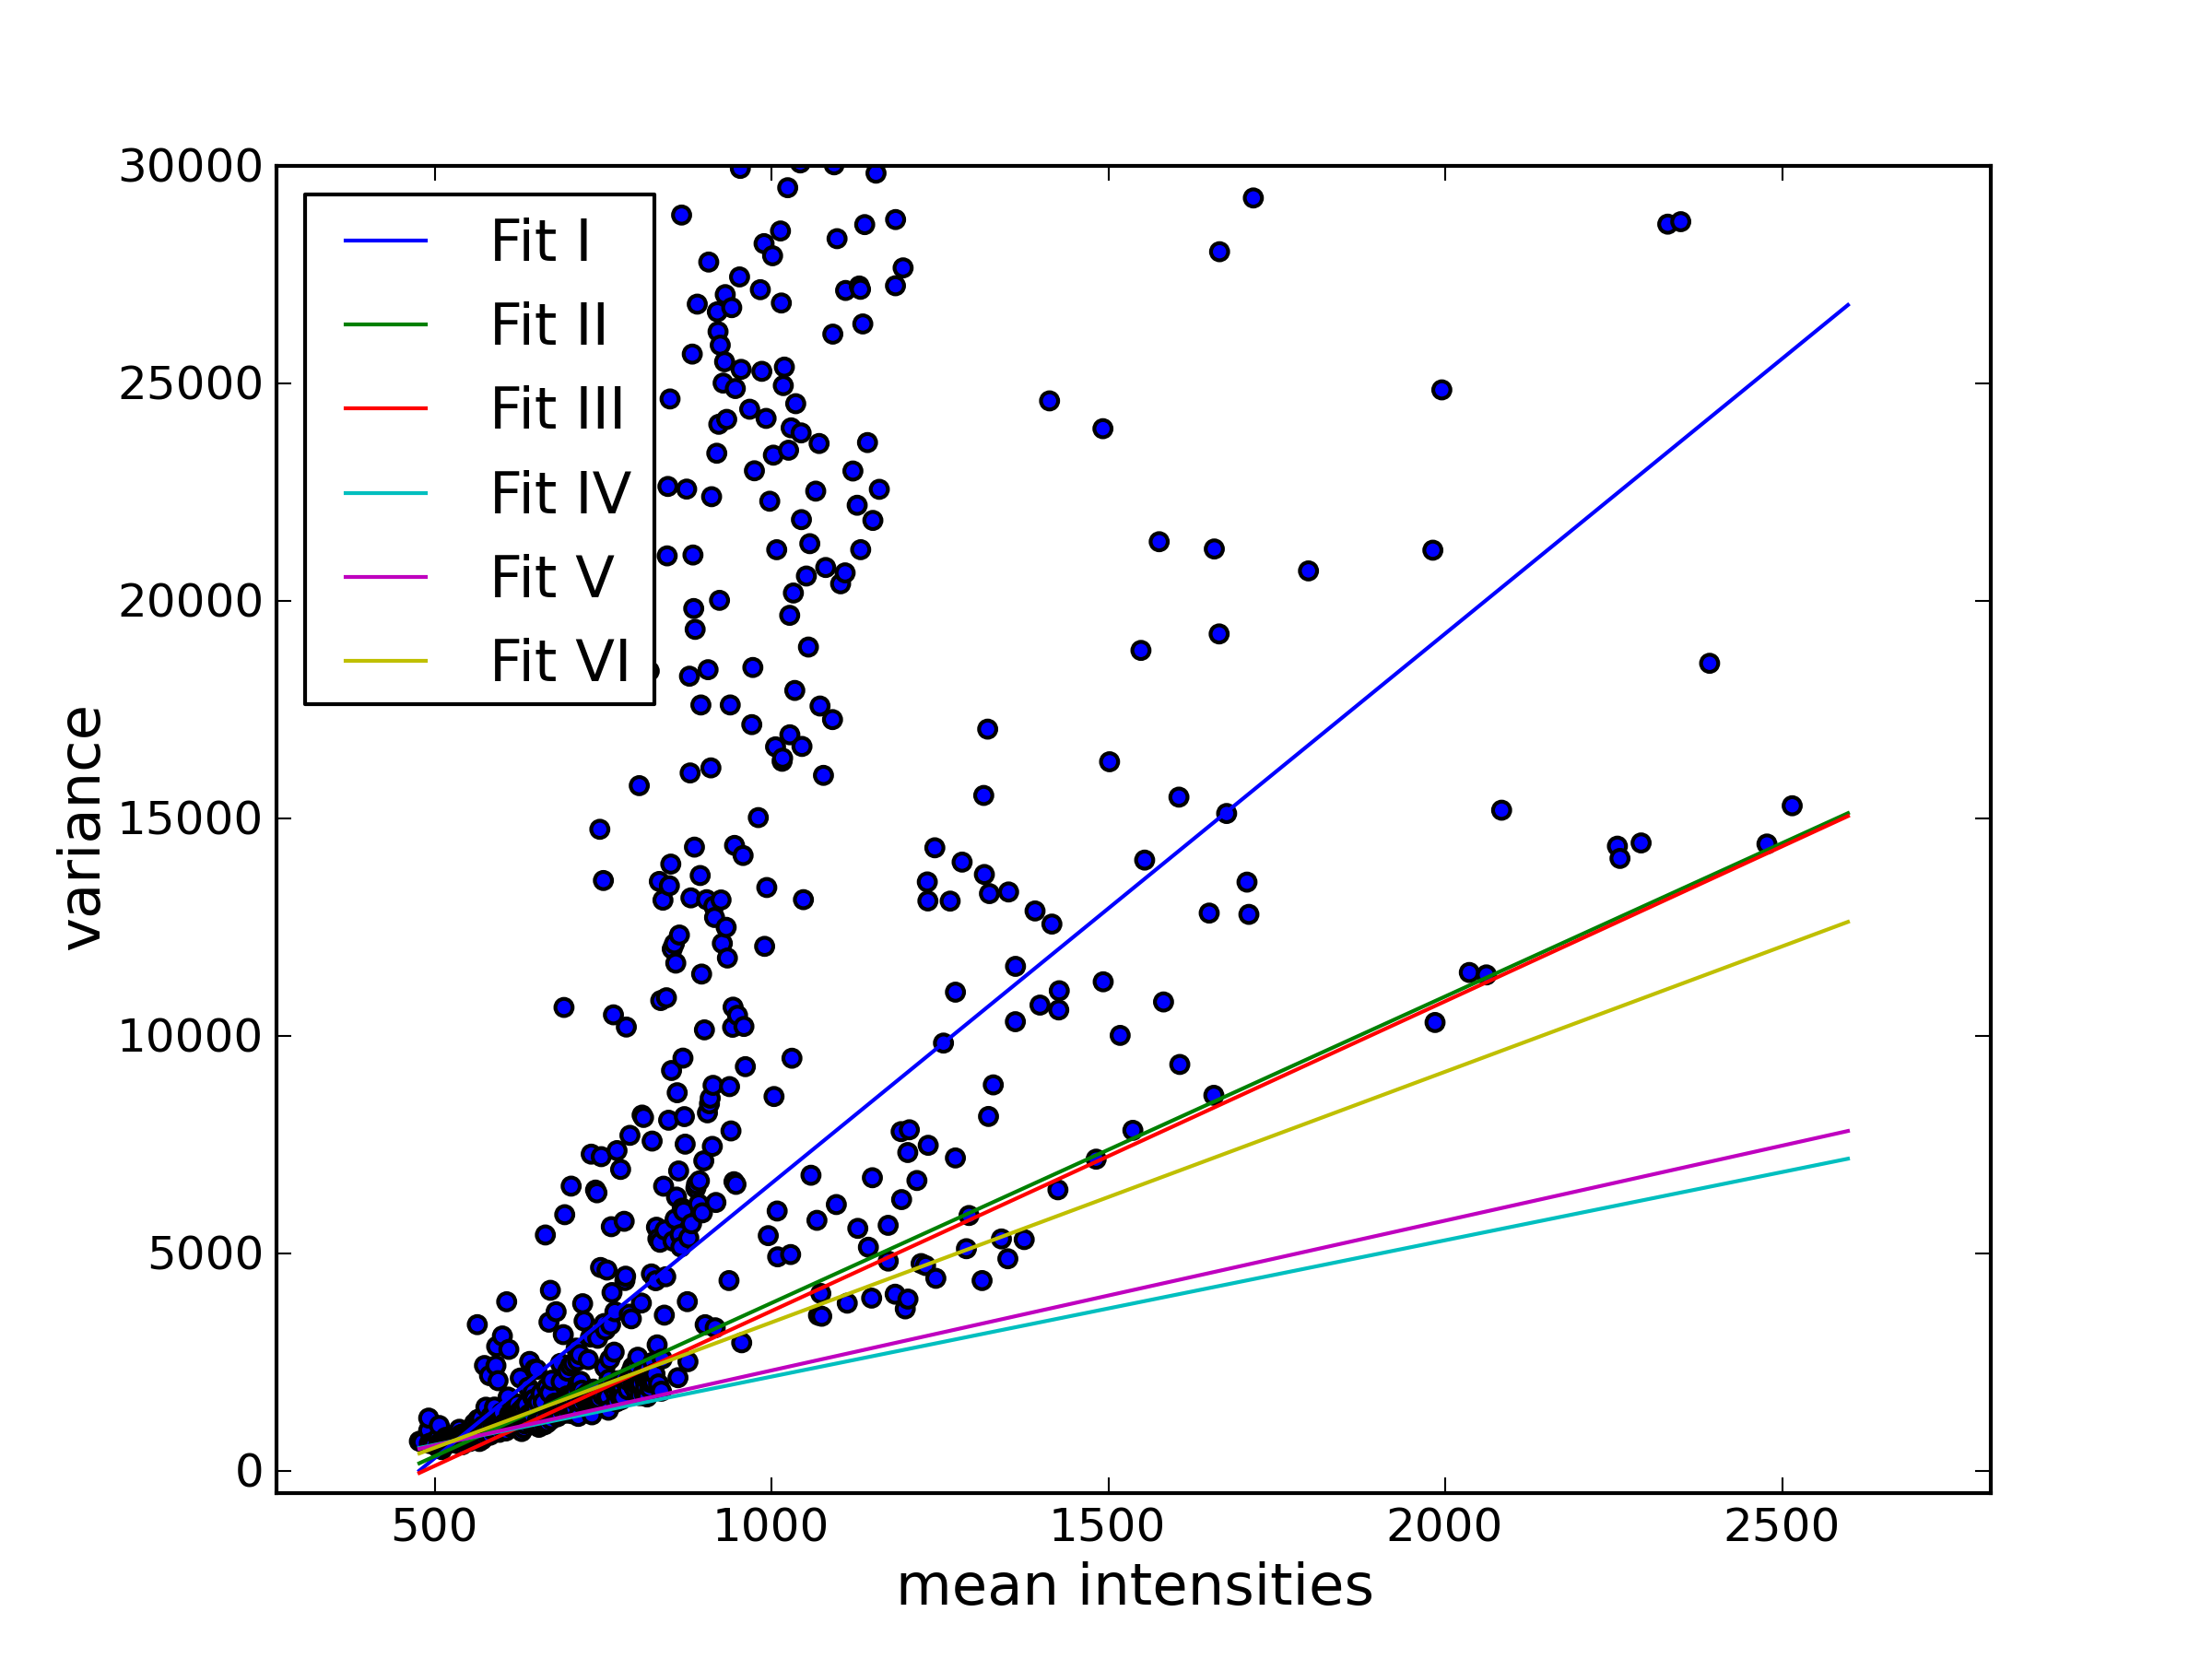
\includegraphics[width =0.48\textwidth]{pictures/geradenplots/pos2green.png}}\\
\subfloat[Pos2\_2\_red]{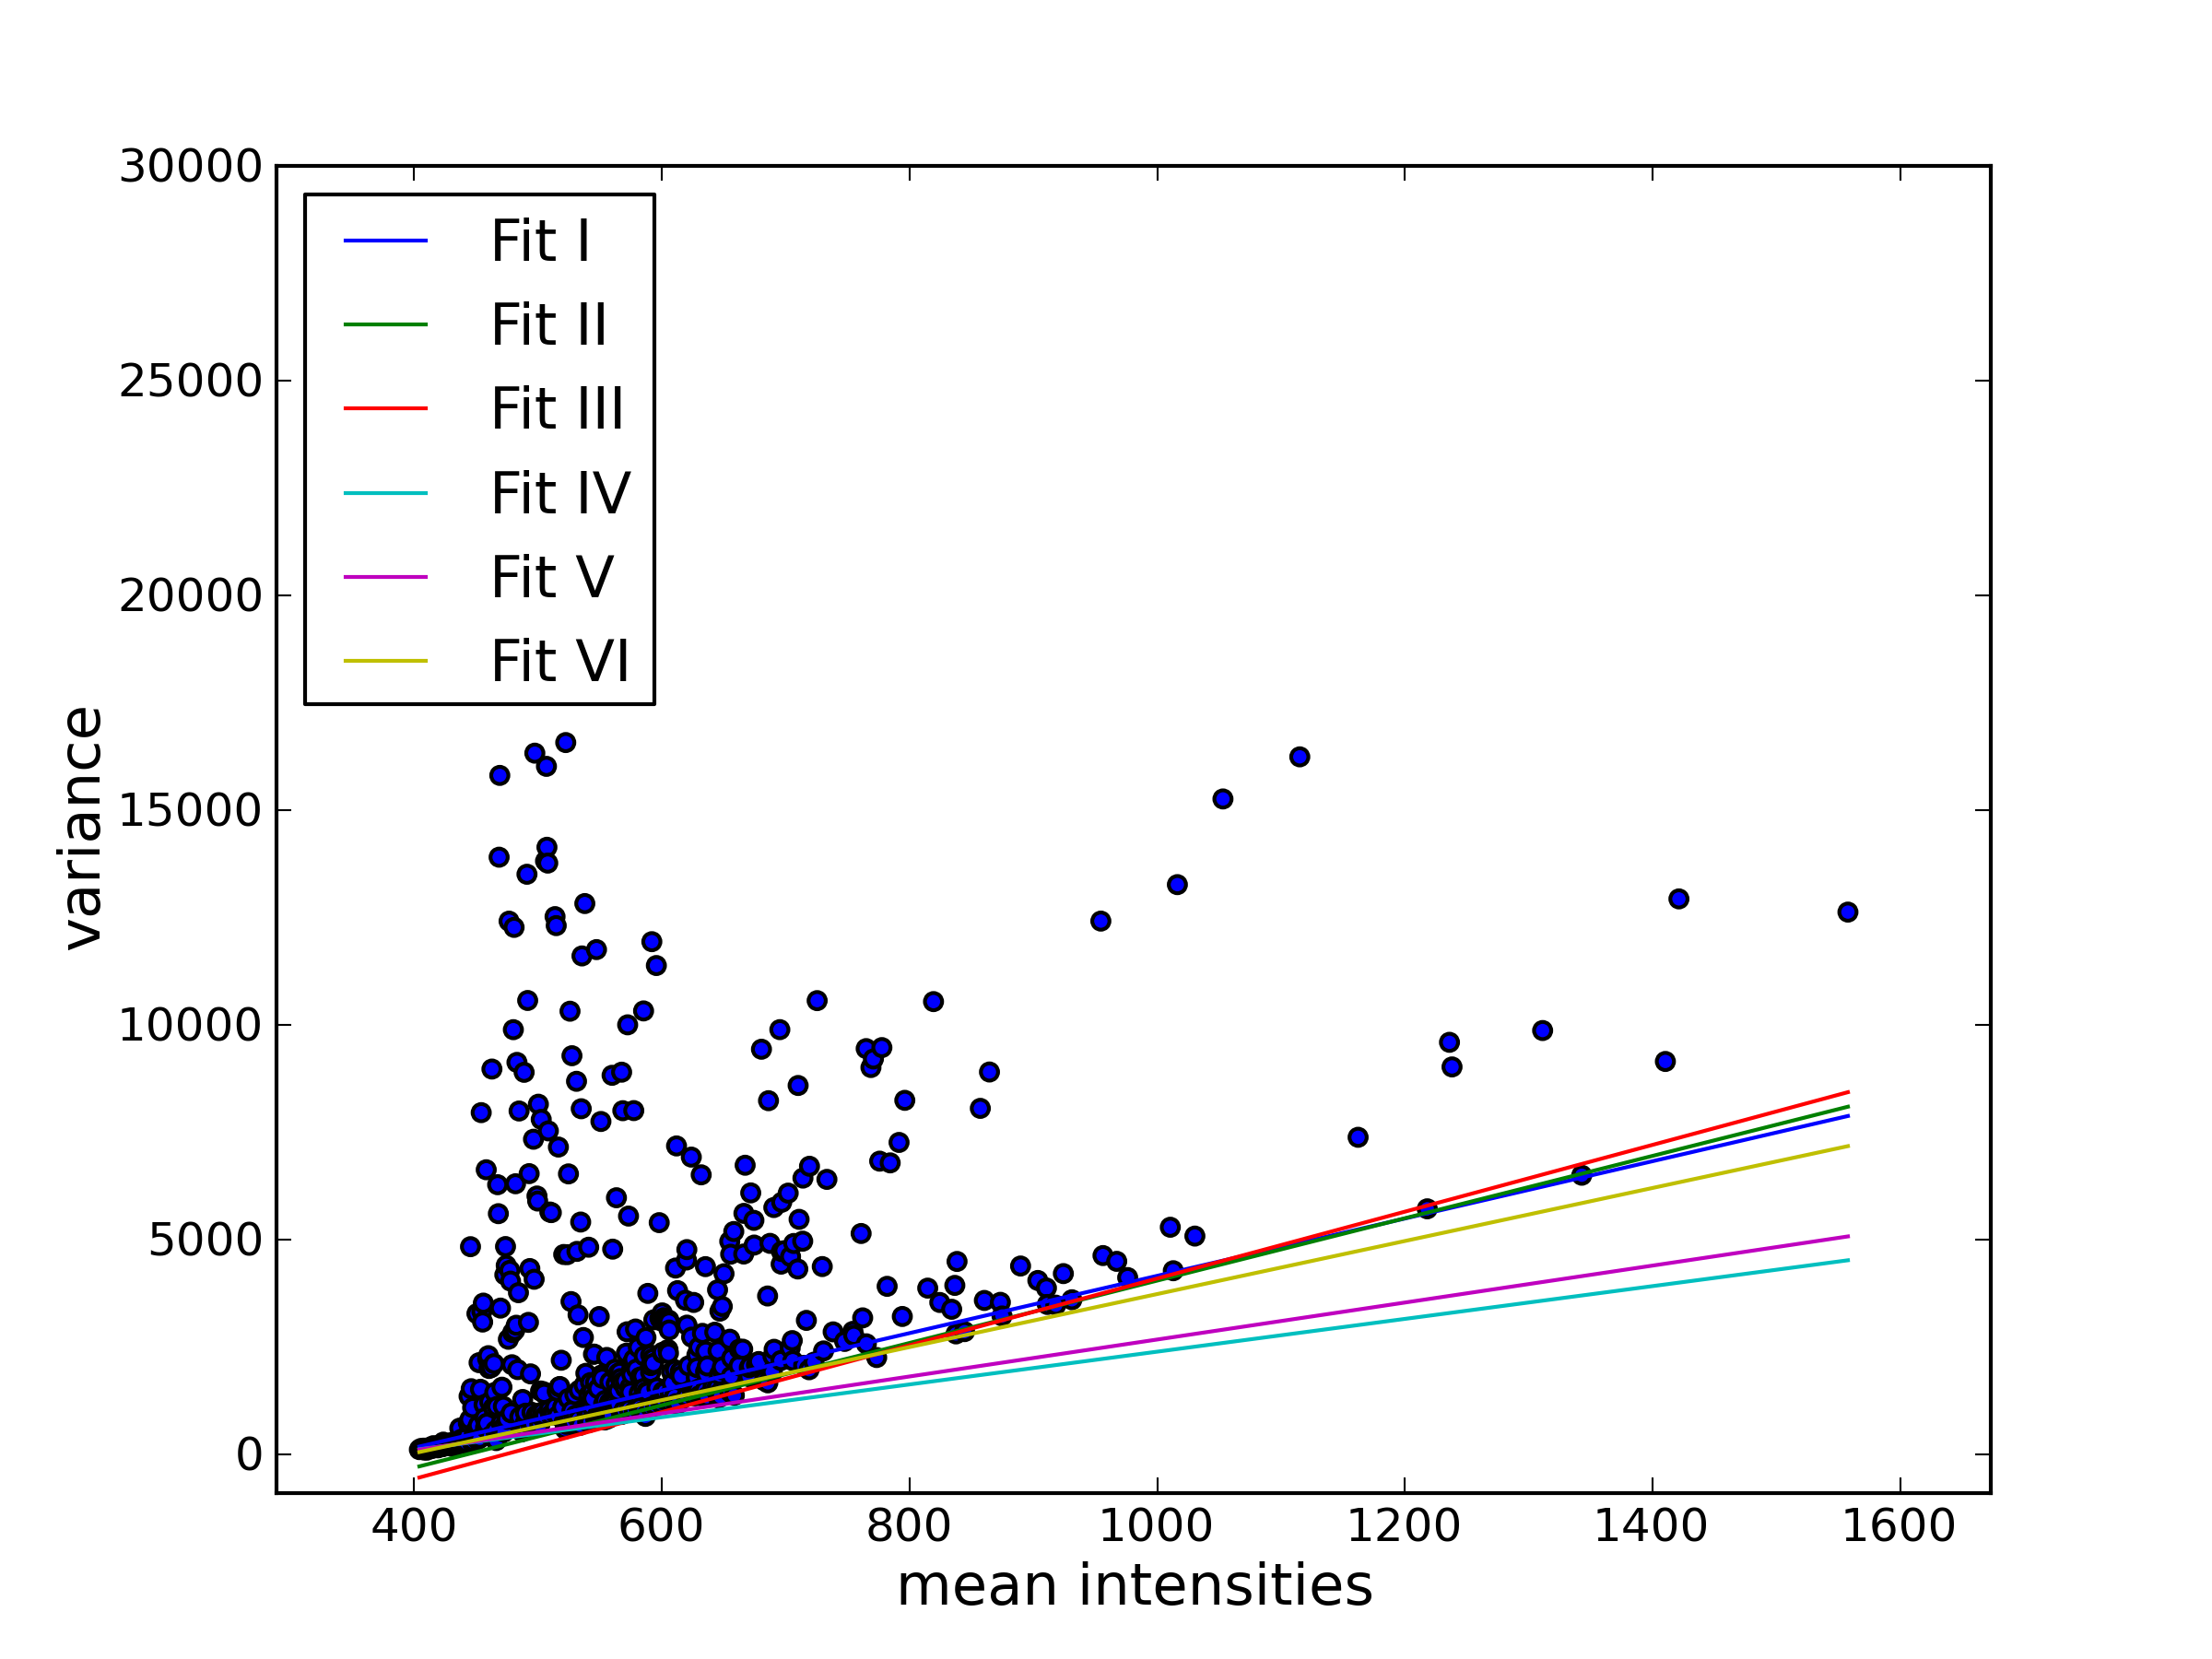
\includegraphics[width =0.48\textwidth]{pictures/geradenplots/pos2red.png}}\hfill
\subfloat[Pos11\_2\_green]{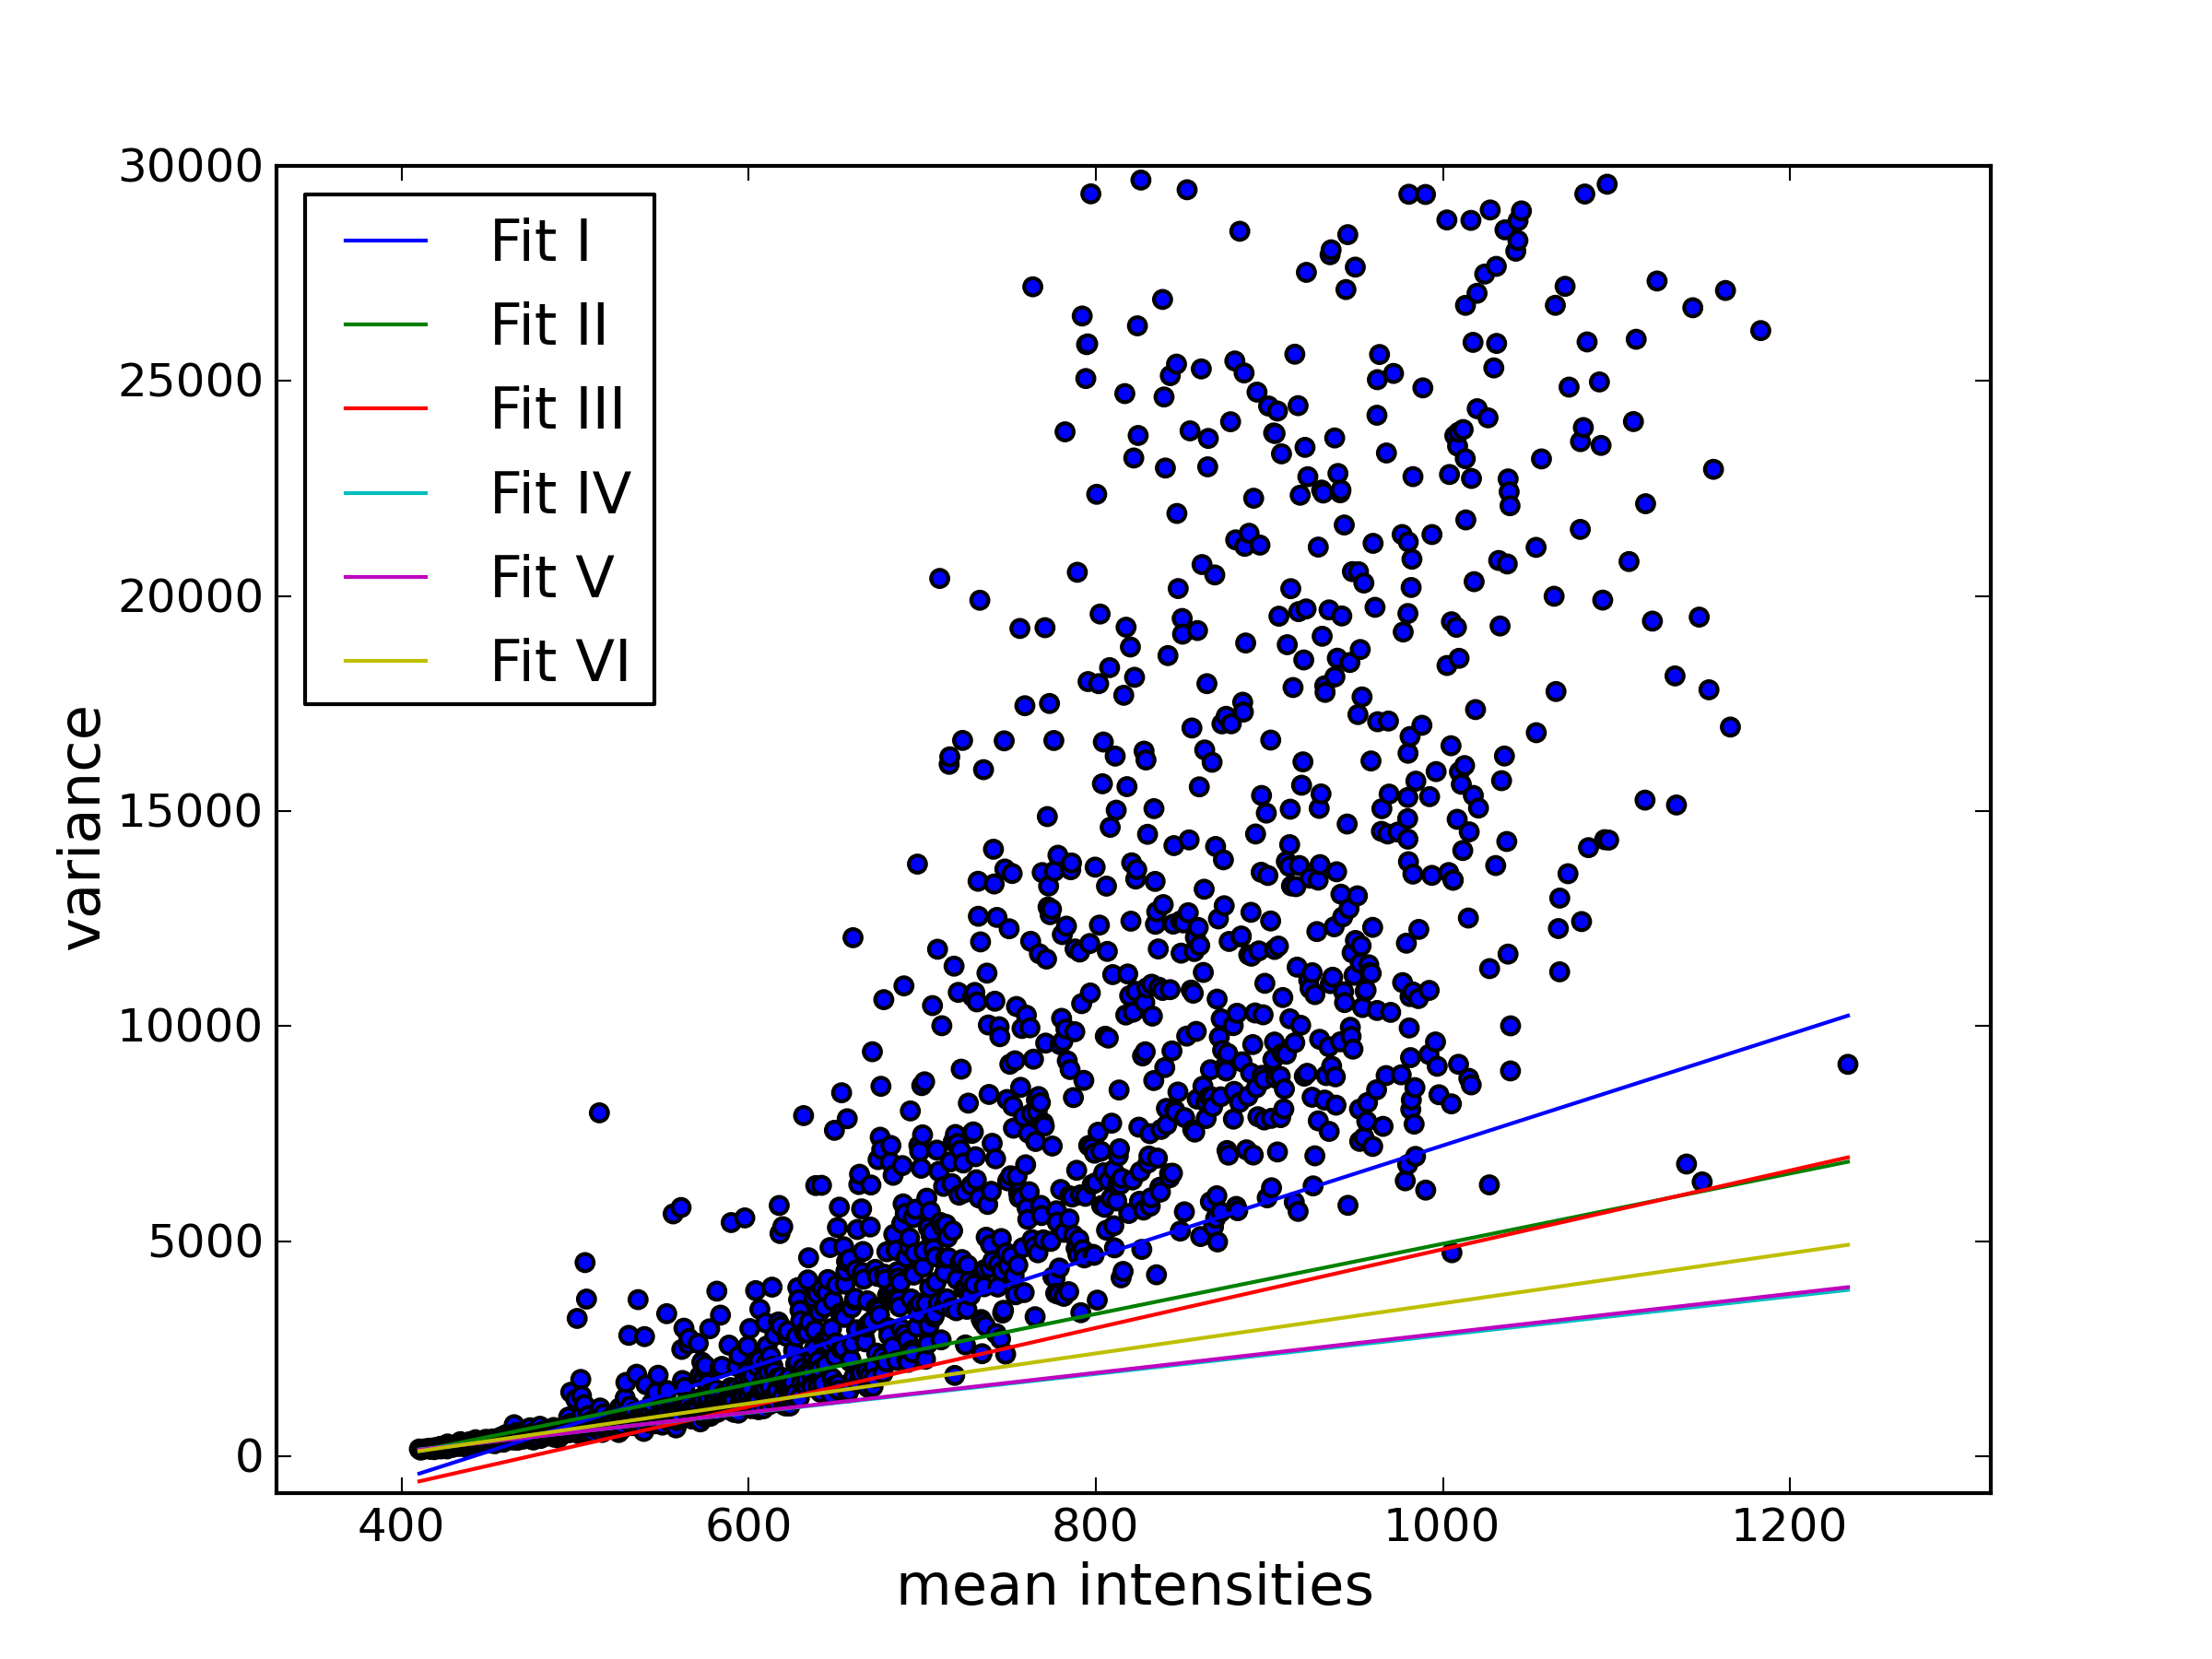
\includegraphics[width =0.48\textwidth]{pictures/geradenplots/pos11green.png}}
\caption{Scatter plot variance over mean for different data sets and the fitting results.}
\label{lineplot1}
\end{figure}

\begin{figure}
\subfloat[Pos11\_2\_red]{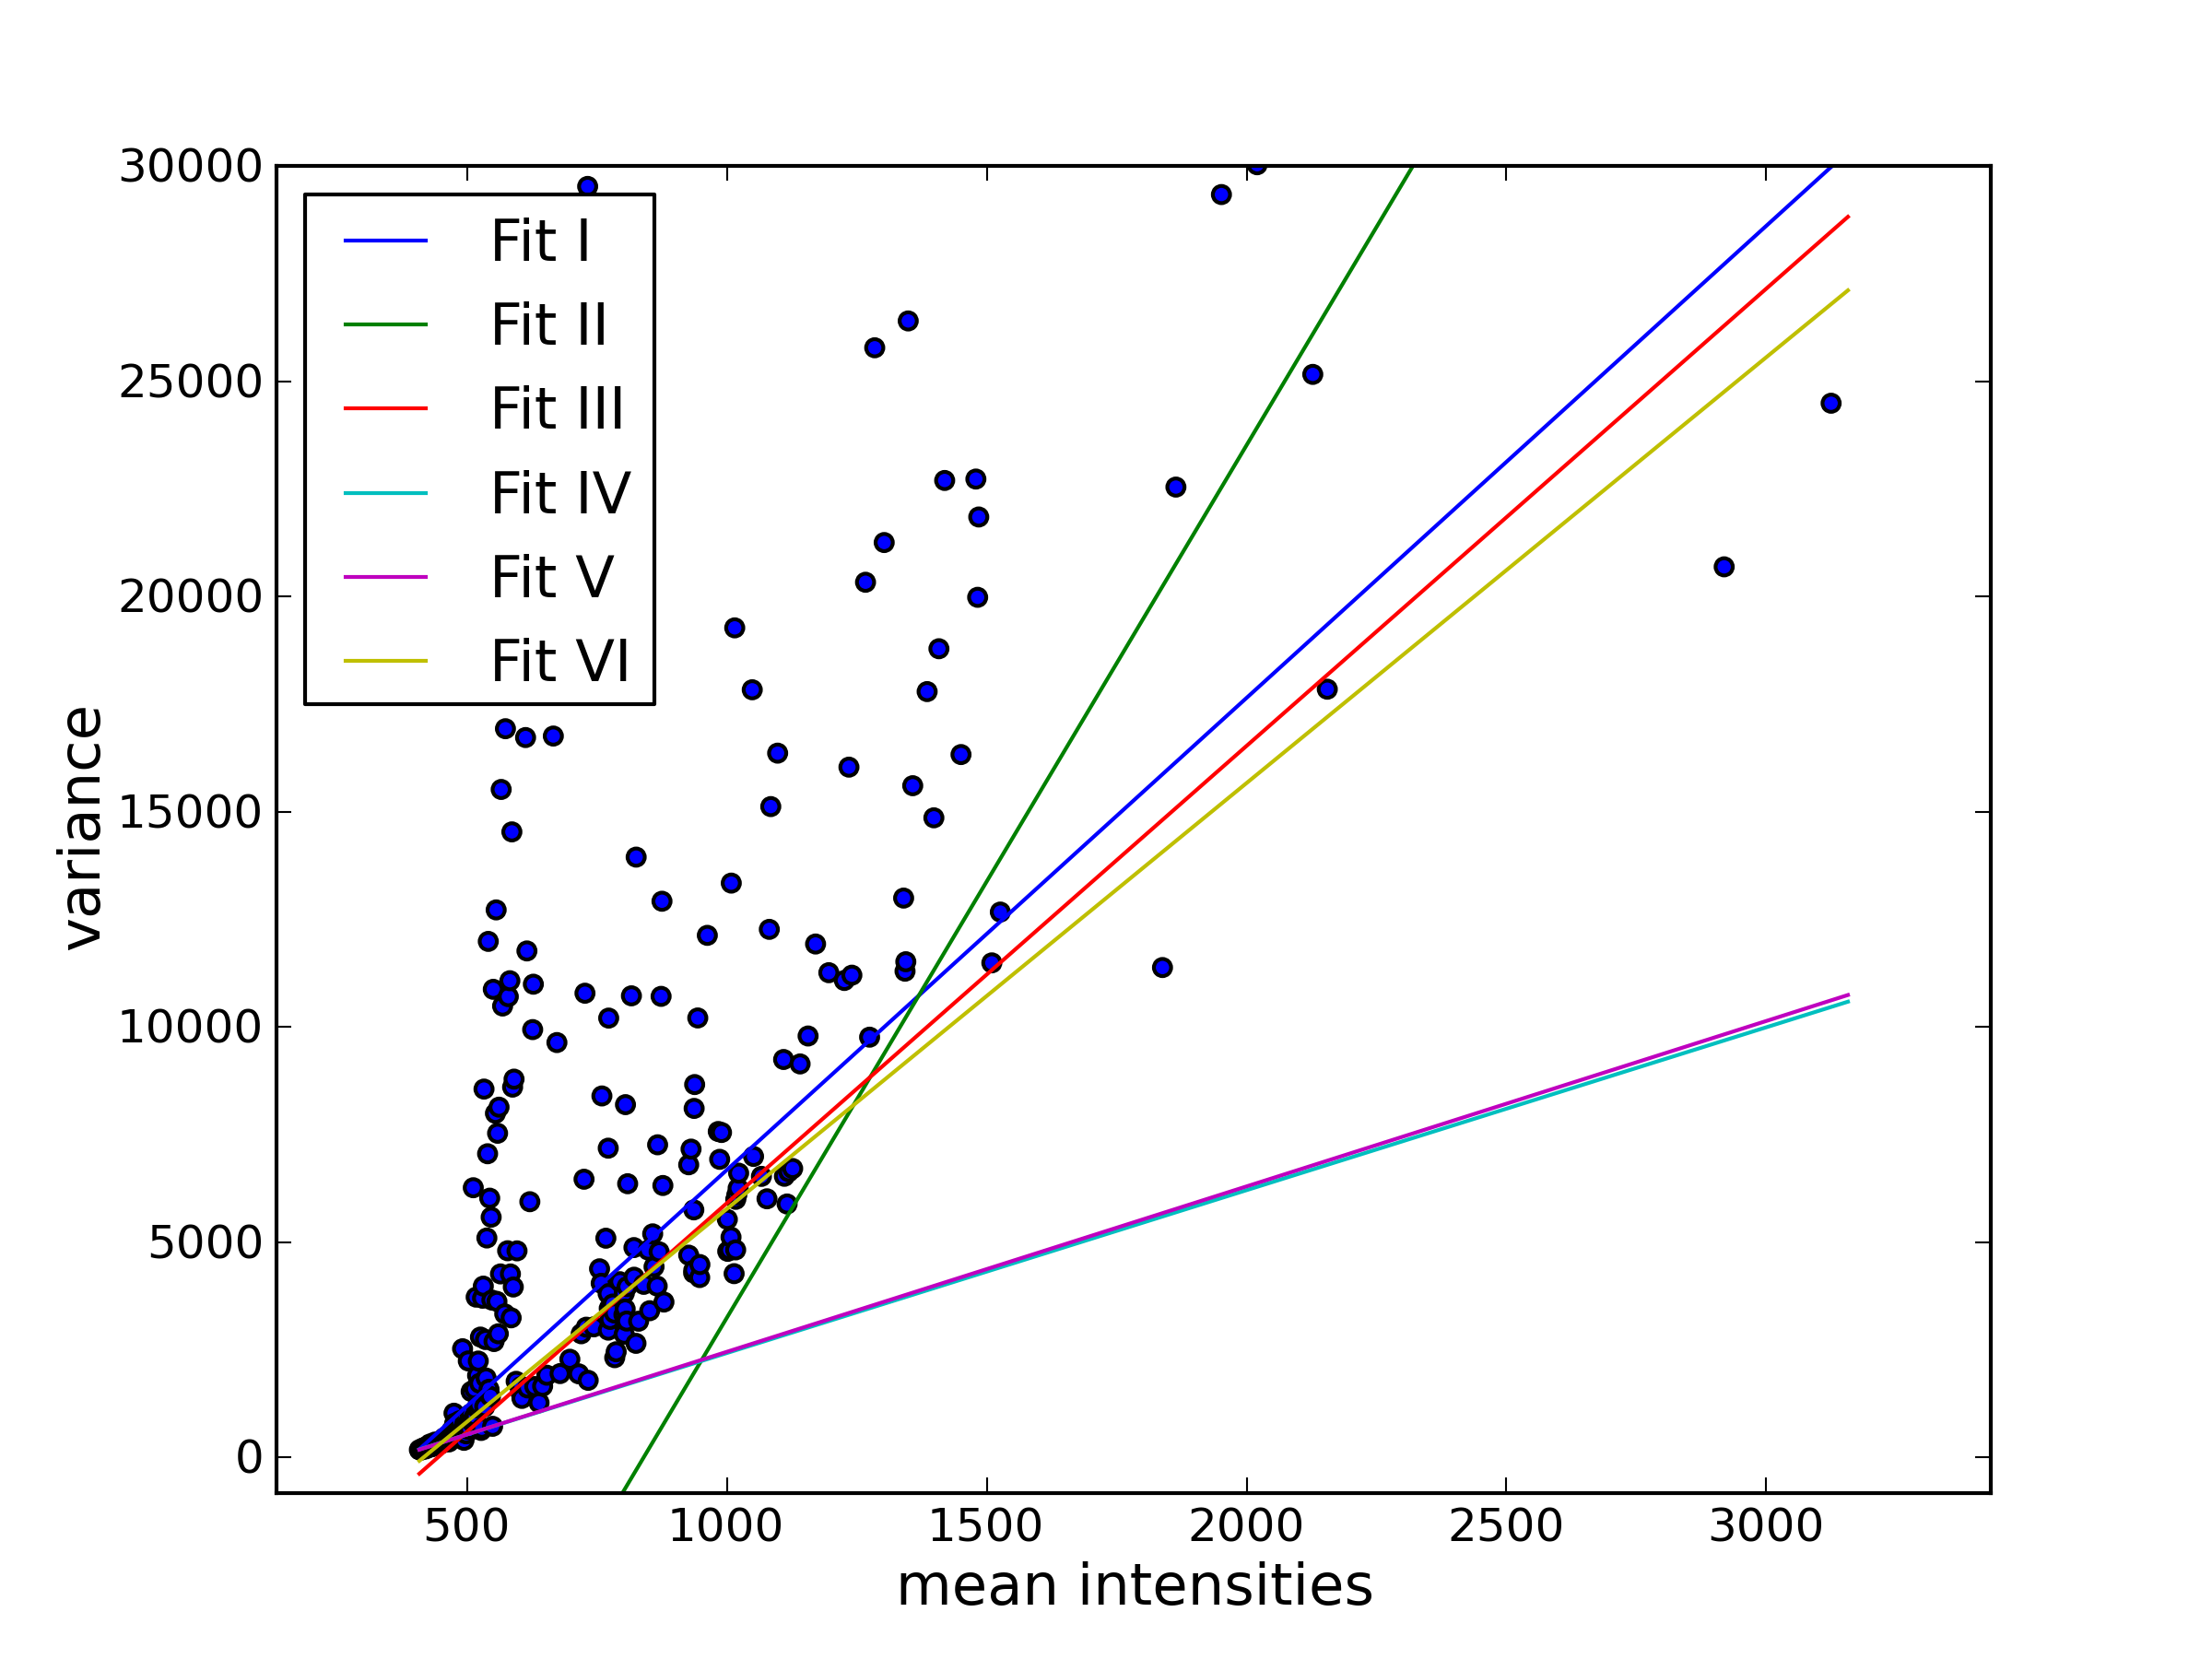
\includegraphics[width =0.48\textwidth]{pictures/geradenplots/pos11red.png}}\hfill
\subfloat[Tetra1\_high\_568]{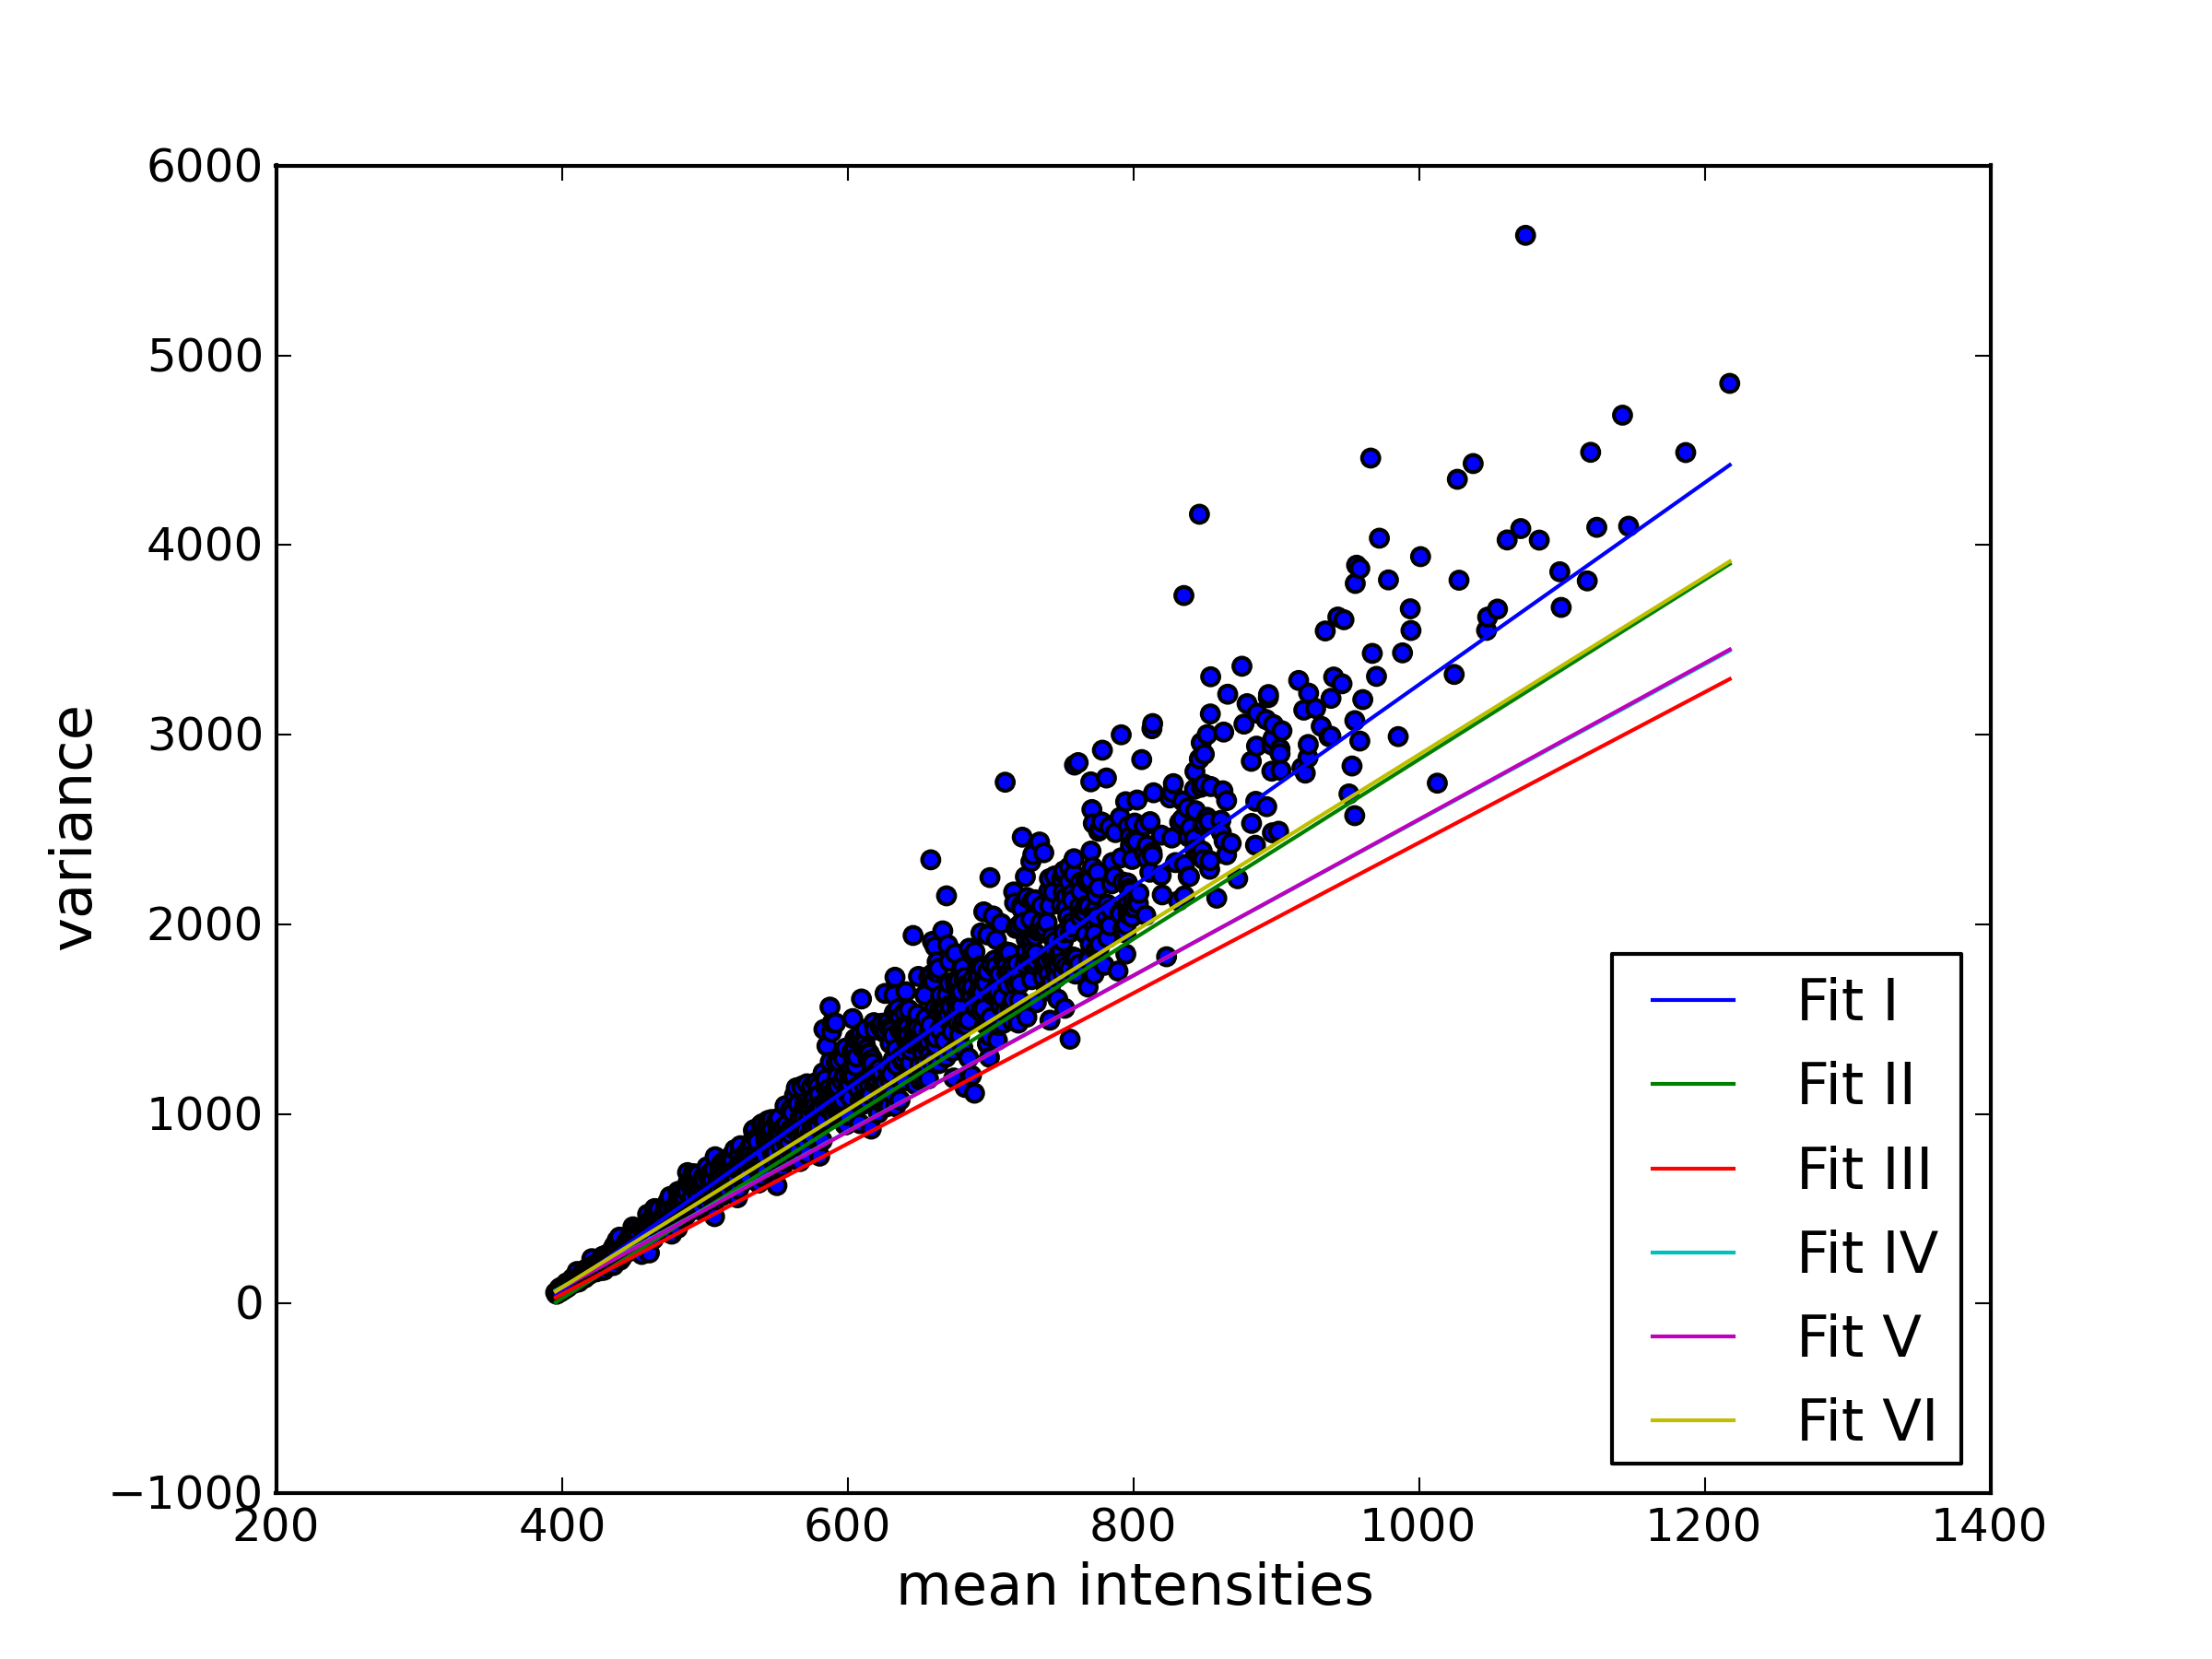
\includegraphics[width =0.48\textwidth]{pictures/geradenplots/tetrahigh568.png}}\\
\subfloat[Tubulin1]{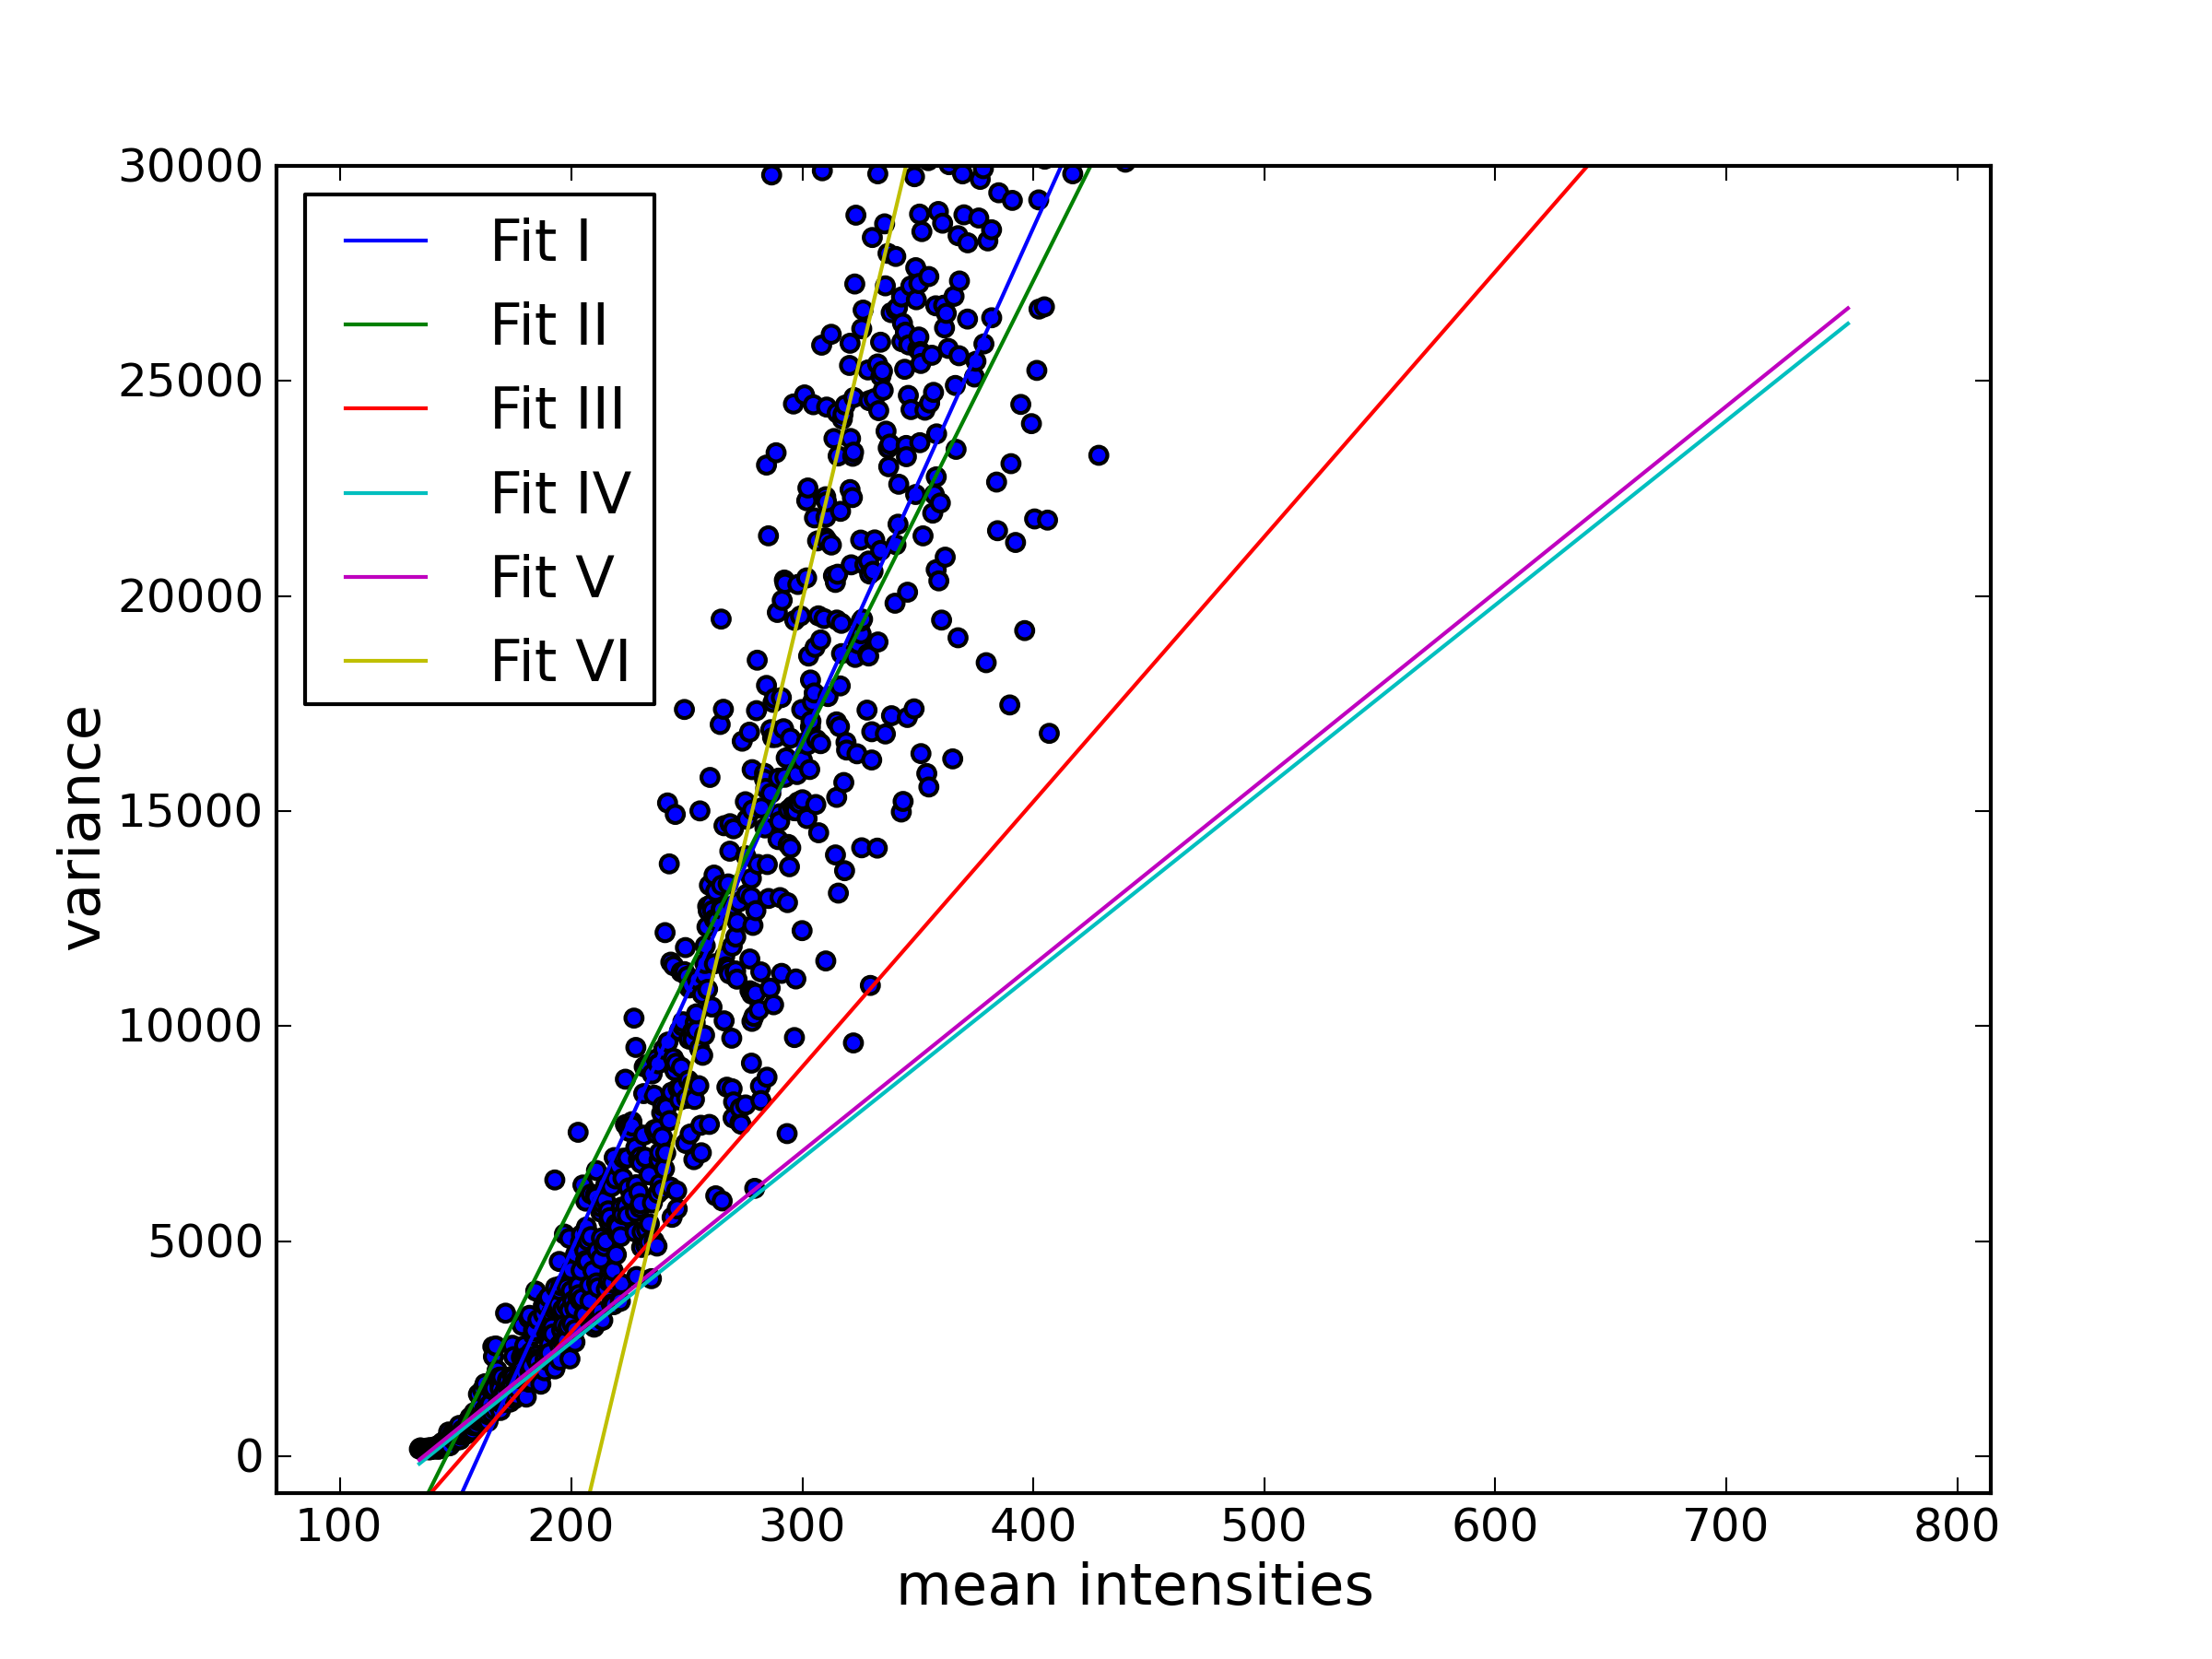
\includegraphics[width =0.48\textwidth]{pictures/geradenplots/bundledtubeshigh.png}}\hfill
\subfloat[Bundled tubes high density]{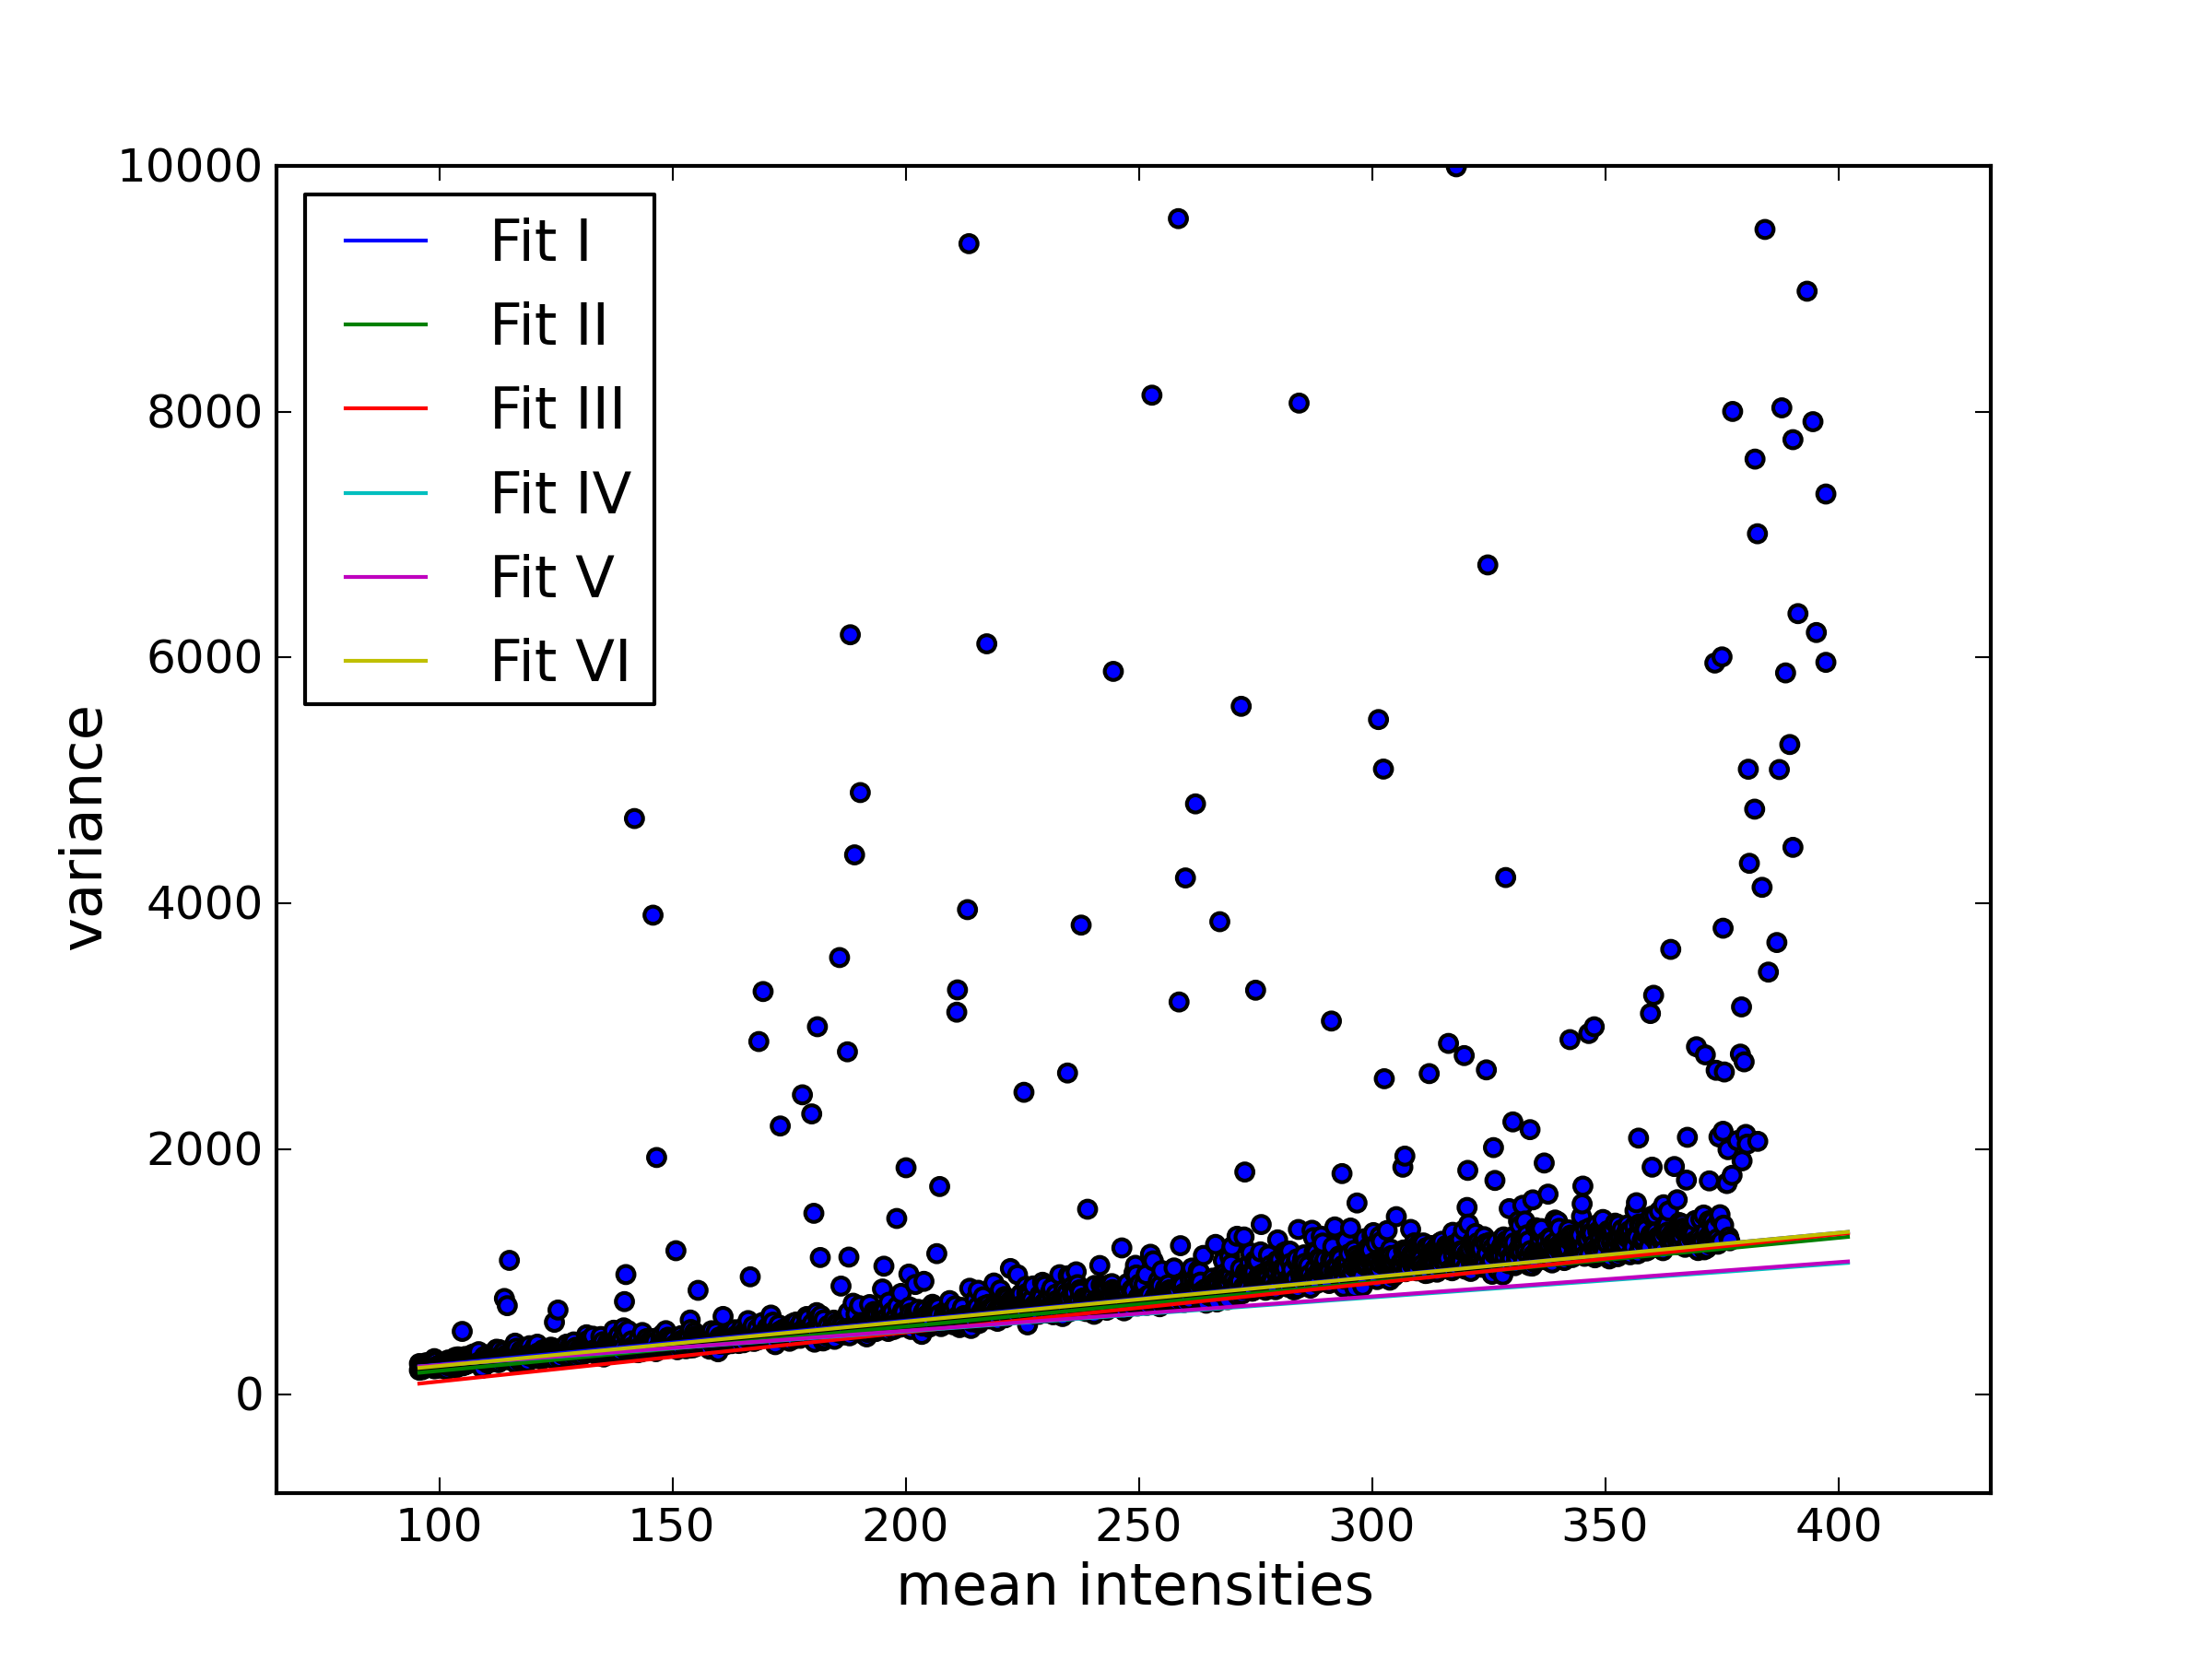
\includegraphics[width =0.48\textwidth]{pictures/geradenplots/tubulin1.png}}
\caption{plot plot2}
\end{figure}
\chapter{Multicolor registration}
Biological samples are often labeled with more than one kind of fluorophore to show different structures within the sample. To align images from
different color channels despite chromatic aberration, beads are used. Beads are
fluorophores added to the probe that emit light of the same wavelengths the
different markers do, and therefore are visible in all channels. The beads can be
used as landmarks, because their position in the aligned image must be the same. The task is to find a transformation that maps corresponding beads on each
other.\newline
The aligned images can then be investigated for colocalized structures.\newline
Both tasks can be done using the improved version of the Colorcomposer.

\section{Chromatic aberration}
In microscopy it is often desirable to label different cell structures with
different colors. To do so our collaborators use different fluoroscent molecules
that emit light at different and therefore distinguishable wavelengths. Using appropriate
filters it is possible to capture pictures containing light emitted from only one
kind of fluorophore.\newline
The propagation speed of light depends on the substance it is propagating through. The property of the substance that describes the ratio of the speed of light in vacuum $c$ and in the substance $v$ is called refraction index $n = c/v$.\newline
The refraction index for any substance depends on the wavelength. Different wavelengths are refracted under different angles. This effect causes the splitting of white light into its components when shining through a prism.\newline
The same effect causes the focal length of the microscope to be wavelength dependent, as sketched in  Figure \ref{wikibild1}. This means that the light for the same spot but with
different wavelengths is not mapped to the same spot in the image. This is the reason why the images of different colors have to be aligned.

\begin{figure}
	\centering
	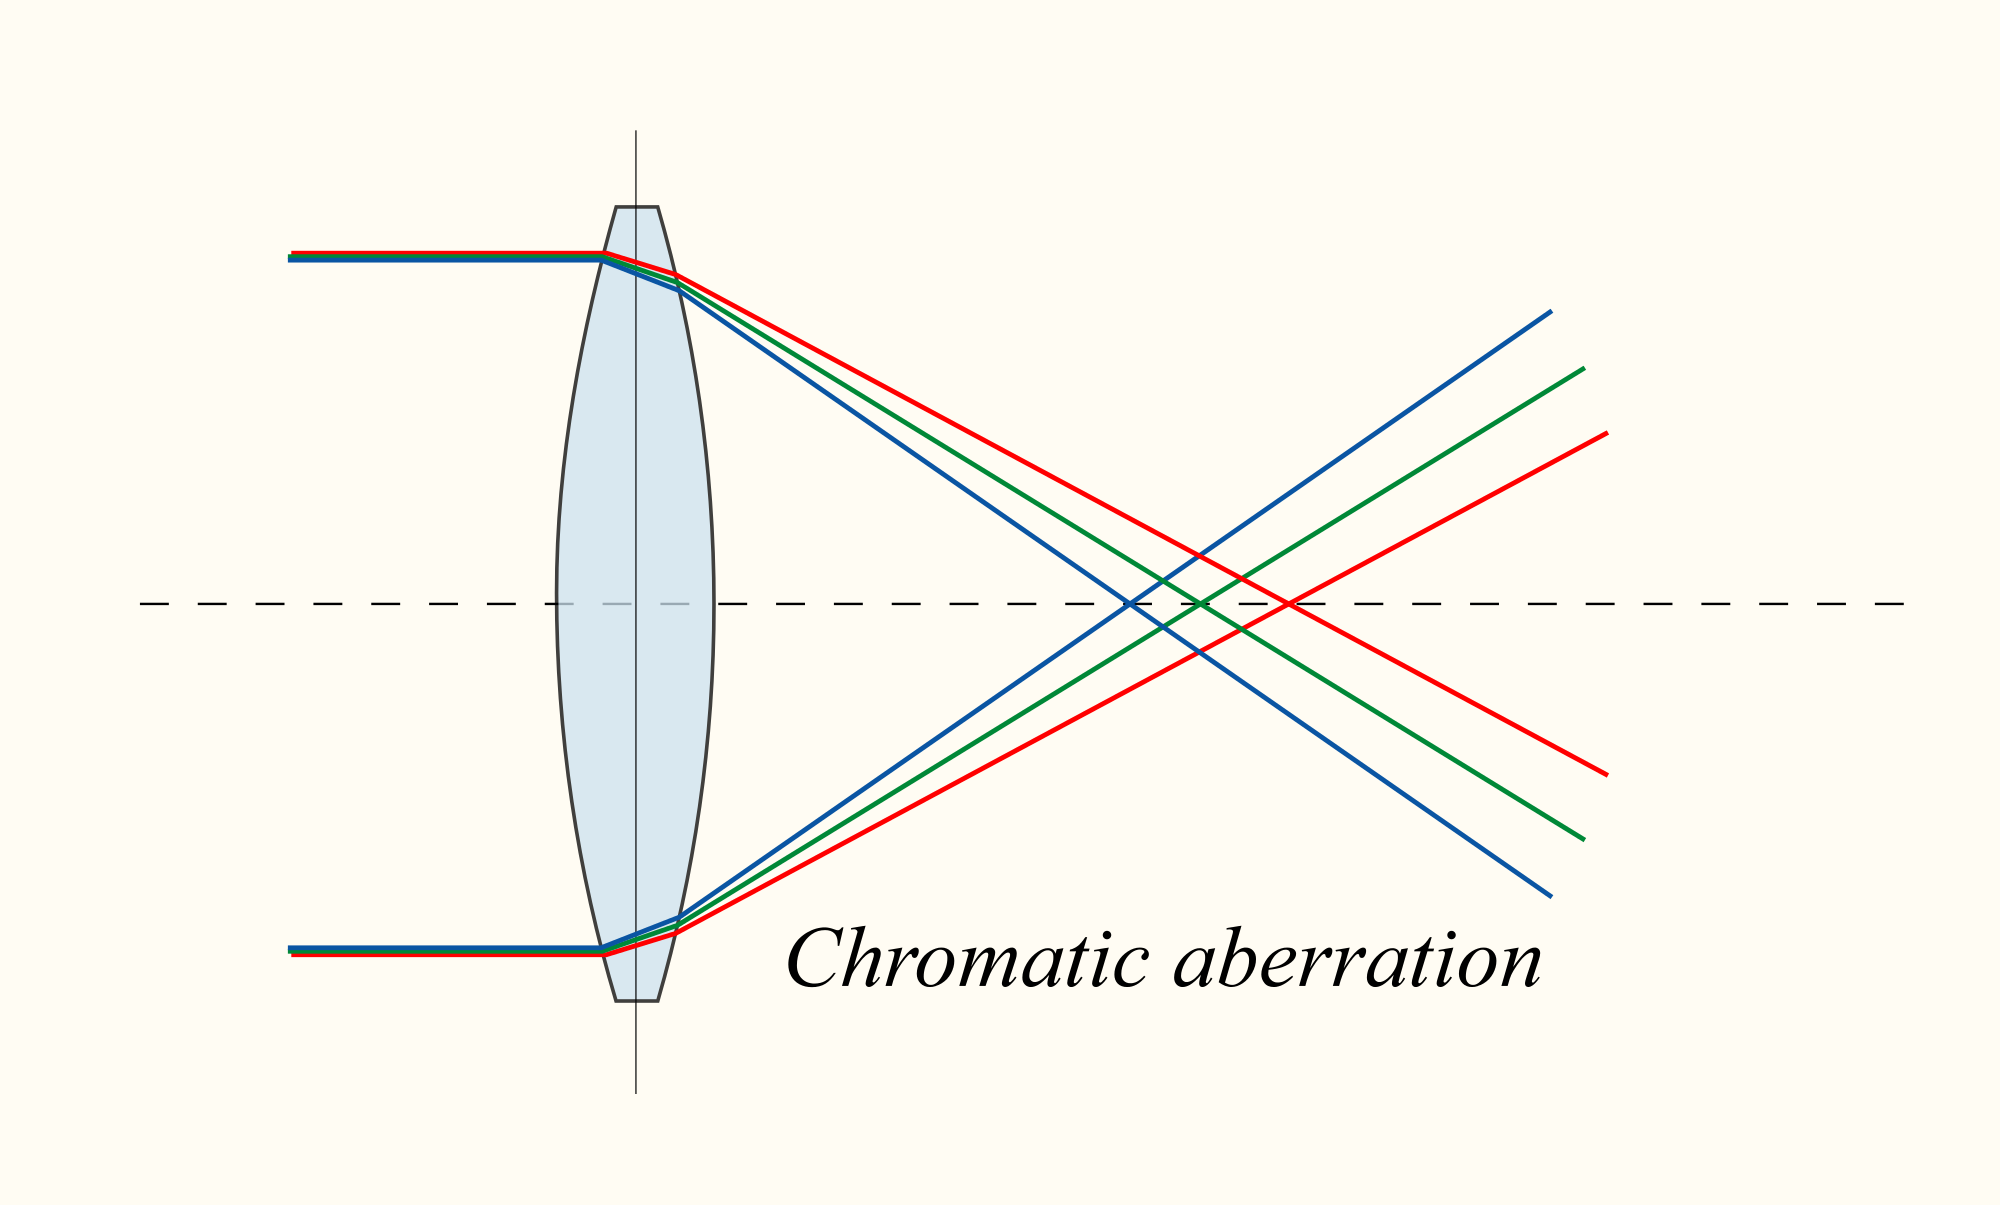
\includegraphics[width = 0.5\textwidth]{pictures/bildabberationwiki.png}
	\caption[Chromatic aberration, picture taken from http://en.wikipedia.org/wiki /File:Chromatic\_abberation\_lens\_diagram.svg, at 23rd of May 2013]{Sketch of the dependency of the focal length on the wavelength.}
	\label{wikibild1}
	\end{figure}


\section{Colorcomposer GUI}
The goal of the Colorcomposer tool is to provide software that is easy to use, flexible and powerful. The current version of the Colorcomposer is easy to use, because the different channels can be aligned by selecting the auto-align option.\newline
Beads can also be manually selected or deleted, if the user wishes to do so. After the transformation the user can use the implemented tool for colocalization detection or save the transformed images and process them with the tool of his or her choice.\newline
The Colorcomposer is powerful as it provides information about the number of points currently under the cursor or their intensities. The estimated transformation error and the localization error are computed and stored.\newline
The basic framework for the Colorcomposer was set up by \cite{MAJoachim}. It contained the workflow for importing and exporting images the handling of bead objects and a linear transformation that used the beads in the order they were found. This early version was unpractical.\newline
Figure \ref{Colorcomposer} shows improved Colorcomposer GUI with two datasets loaded. The buttons on the right give the user the option to add or remove beads in addition to the autodetected beads. There are different sliders to control the values used for bead detection. In the lower right corner additional information is provided about the total number of points within a rectangle with the selected cursor radius' size. The sum of the intensities and the total number of frames for each data set are also given. This information is helpful to determine whether a cluster of points is a bead or not.\newline
At the top there is a menu bar with new options, that enable the user to discard all beads, automatically detect beads, calculate colocalization measures and show or hide the colocalization heatmap.
\begin{figure}
\centering
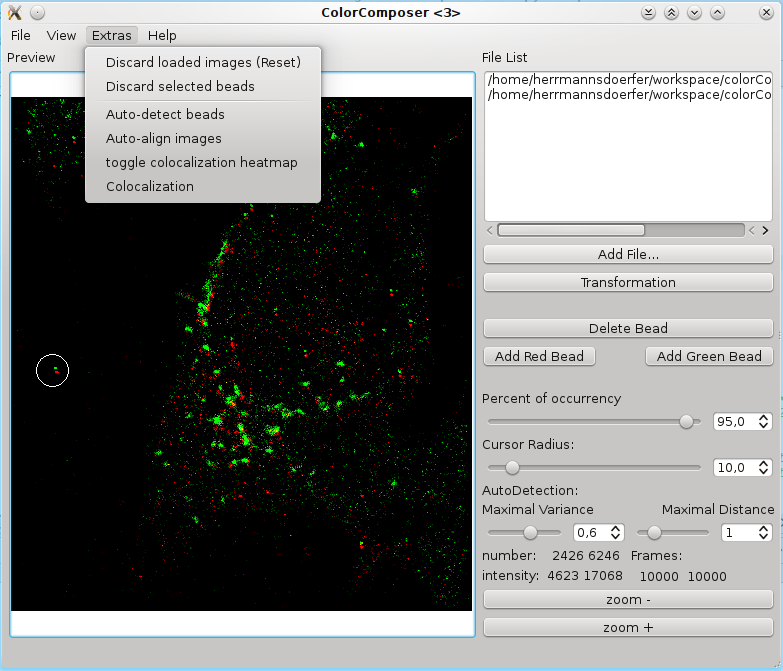
\includegraphics[width = 0.88\textwidth]{pictures/GuiColorcomposer/BeforeAlignmentWithMenu.png}
\caption{Improved Colorcomposer GUI. On the right are the sliders to set the parameters. There are also buttons to add or delete single beads. In the lower right additional information about the area under the cursor is displayed, such as numbers of pixels, total intensity and the number of frames in total.}
\label{Colorcomposer}
\end{figure}


\section{Features of the Colorcomposer application}
\subsection{Invariance of input data units}
The resulting coordinate files from SimpleSTORM or other STORM algorithms may be given in units of pixels relatively to the unprocessed data or in nanometers. Treating coordinates given in nanometer as pixel units would lead to very huge and very sparse images displayed in the Colorcomposer. Therefore the Colorcomposer reads out additional information from the coordinates text files header. These information are the pixel to nanometer ratio and the used factor. With this information the picture can be reconstructed as an upsampled version of the input image by the used factor, regardless of the units used to save the coordinates file. If none of this information is given a pixel to nanometer ratio of 1 is assumed which guarantees backward compatibility with older coordinate files given in pixel units.
\subsection{Manual bead selection and removal}
With the improved version of the Colorcomposer it is possible to add beads manually. To do so the desired location is clicked in the preview image and after that either the button "add green bead" or "add red bead" is hit. If there are enough frames containing localizations near the given location a bead is added to the center of mass of the intensities in that area. If the button "delete bead" is pressed all beads in the selected area are deleted.\newline
This feature can be used to add beads missed by the automatic bead detection.
\subsection{Automatic bead detection}
The input for the Colorcomposer application is a text file created by the storm
algorithm that contains information about the position, intensity, symmetry,
frame number and signal-to-noise ratio of each detection. The beads should
ideally appear in most of the images. This means they can be found by searching for
detections that appear in almost every frame at the same position.\newline
There was already an automatic bead detection implemented by Joachim Schleicher. This was improved as follows.\newline
All important parameters for the bead detection can now be set in the GUI. The bead detection works by searching for points that appear in most of the frames. Instead of taking all localizations from the first frame as expected bead positions without considering locations that do not appear in the first frame, now a good subset of positions from the first 50 frames is found. This is done by skipping redundant positions based on the minimal distance of a new position to all positions already in the set. The range of 50 frames to look for beads is sufficient because it is very unlikely that all 50 detections of the bead have been missed.\newline
After good candidates are found their number of points, variance and mean position is determined like described by \cite{MAJoachim}.\newline
In the end beads that are too close are merged to a new bead with its center right between the merged beads.

\subsection{Alignment of two multicolor images}
After the beads for each channel are found, the next task is to find the corresponding
beads in each channel. It happens that some beads only occur in one channel.
If this happens there will be no corresponding bead in the other
channels.\newline
The first step is to discard beads that are far away from any bead of the other color. From the resulting subset of beads the maximal number of possible bead pairs is estimated by taking the smaller number of beads per color.\newline
The iteration begins that tries to find the best transformation to map all beads from one color to the beads of the other color. Therefore all beads from the color with less beads are chosen and the same number from the other color are selected. This selection is based on
a probabilistic approach and the distance matrix containing the information about the
distances between all beads of the two channels. It is more likely for nearer beads of the other channel to be selected, but any bead within a certain range can be chosen.\newline
Using these pairs of beads, a linear transformation is found, as described by
\cite{MAJoachim}.\newline
This transformation is used to test how many other beads, that were not used to calculate the transformation match. It is assumed that the correct transformation will match additional bead pairs. 
This step is repeated multiple times.\newline
The maximal number of matching bead pairs is compared with the number of assumed bead pairs. If less bead pairs are found than expected the number of expected bead pairs is reduced by one and the previous procedure is repeated with the appropriate number of beads randomly chosen from the channel with less beads.\newline
All transformations that match more or equal bead pairs are stored. Also all bead pairs that are aligned under these transformation are stored. The number of assumed bead pairs is reduced by one and the iteration started again. \newline
This loop ends when the assumed number of bead pairs is lower than 3, the minimal number of bead pairs necessary for the calculation of the transformation.\newline
All candidates for the transformation are checked for the occurrence of shearing.
In principle shearing should also be allowed for a linear transformation, but tests
indicate that shearing does not occur, so it is disabled to improve stability. \newline 
If there are only
three beads in each channel used for the transformation, then a perfect transformation is found every time,
but the correct one, if possible, is the one without shearing. There will be another problem with this transformation if the bead density is very high it is possible that a transformation with much shearing is found. This compresses the beads of one channel to a slim band. The probability to find a matching point by chance is much greater then. \newline
Figure \ref{badshearing} shows the result of an incorrect transformation of simulated data. The red channel was created by randomly placing beads. The green channel was slightly shifted and rotated. The green channel was transformed to match with the red channel. Only a subset of beads was used to calculate the transformation and so this solution was found and chosen from the algorithm because of the additional matching point.\newline
These effects can be suppressed by not allowing shearing for the transformation.

\begin{figure}
\centering
\includegraphics[width = 0.95\textwidth]{pictures/shearingBad2.png}
\caption{Affine transformation with shearing enabled. The green channel is deformed and one bead matches by chance which led to selection of this transformation. The beads that match are highlighted.}
\label{badshearing}
\end{figure}
\subsection{Information about localization certainty}
The detected spots from SimpleSTORM contain some localization error. This error was derived in section \ref{detectionError}. It depends on the signal-to-noise ratio and the scale of the point spread function of a single fluorophore.

Within all transformations that do not show shearing, the transformation is chosen that has the least root mean square error for all matching pairs of beads.

\section{Total localization error}
There are four contributions to the total localization error considered in this thesis.\newline
First there is the error that arises from the linear transformation to align the beads. To estimate this error the variance of the estimator is used. Since the transformation matrix is calculated by linear regression from the matrices $B$ and $R$ of the localizations of the first and the second layer of beads, with $B$ being the matrix of the first layer to that the second layer $R$ is transformed to. The variance of the estimator is
\begin{align}
\text{variance registration}&= \sigma^2 x_0\left(R^TR\right)^{-1}x_0^T, \text{ with }x_0 = \left(x_0,x_1,1\right) \label{gl22}
\end{align}
Using equation \ref{gl22} the variance $\sigma^2$ for all pixel can be calculated.\newline
The second contribution to the total localization error is the localization error of the SimpleSTORM algorithm. Its formula is
\begin{align}
 \text{variance localization} = \frac{N^2\pi}{2S_0^2} \left(1+\frac{\sigma_\text{PSF}^2}{\sigma_\text{filter}^2}\right)^2\left(\sigma_\text{filter}^2+\sigma_\text{PSF}^2\right)^2
\end{align}
It is derived in \ref{detectionError} and can be calculated for each detection individually based on the known signal-to-noise ratio. The signal-to-noise ratio gives directly the signals intensity $S$, because of the known noise variance of one which gives the nois' standard deviation $N$ of also one. The PSFs width was either given or estimated and is passed to the Colorcomposer in the detection coordinate file's header along with the prefactor $f$ for the actually used filter. Using this the localization error can be written as
\begin{align}
 \text{variance localization} &= \frac{N^2\pi}{2S_0^2} \left(1+\frac{\sigma_\text{PSF}^2}{f^2\sigma_\text{PSF}^2}\right)^2\left(f^2\sigma_\text{PSF}^2+\sigma_\text{PSF}^2\right)^2 \\
 &=\frac{N^2\pi}{2S_0^2}\left(1+\frac{1}{f^2}\right)^2\left(1+f^2\right)^2\sigma_\text{PSF}^4\\
 &= \frac{N^2\pi}{2S_0^2}\left(2+\frac{1}{f^2}+f^2\right)^2\sigma_\text{PSF}^4
\end{align}
The third contribution results from the fact that the fluorophors are not directly attached to the sample of interest, since the antibodies used for staining are in between. The upper bound of this error can be estimated under the assumption that the target of the antibodies is much smaller than the antibodies, so that there is no occlusion in the projection. This assumption does not hold in reality. Structures like cell membranes are certainly larger than the antibodies, but the assumption gives an upper bound. 
\begin{align}
\text{variance position} &=\frac{1}{\Omega_\text{Sphere}}\int\limits_{\Omega_\text{Sphere}} x^2 dV\\ 
&=\frac{1}{\Omega_\text{Sphere}}\int\limits_0^{2\pi}\int\limits_0^\pi R^2\sin\theta \left(R\cos\phi \sin\theta\right)^2 d\theta d\phi\\
&=\frac{R^2}{4\pi} \int\limits_0^{2\pi}\int\limits_0^\pi \cos^2\phi \sin^3\theta d\theta d\phi\\
&=\frac{R^2}{4\pi} \left[\frac{1}{2}\phi +\frac{1}{4}\sin 2\phi \right]_0^{2\pi}\int\limits_0^\pi \sin^3\theta d\theta \\
&=\frac{ R^2}{2} \left[\frac{1}{12}\cos3\theta -\frac{3}{4}\cos\theta \right]_0^\pi=\frac{2}{3} R^2
\end{align}
$R$ is the assumed distance of the fluorophore to the structure it is attached to (about 20~nm/0.09~px).\newline
The fourth and minor contribution to the total localization error for each pixel is the quantization noise. It occurs when continuous intensities, as the photons forming the PSF, are transformed into integer values. Quantization noise describes the round-off error. The round-off error can be any value between -0.5 and 0.5 and is uniformly distributed. Its variance is
\begin{align}
 \text{variance quantization} =\int\limits_{-\frac{1}{2}}^{\frac{1}{2}} x^2 dx = \frac{1}{12}
\end{align}
The unit of this error is the pixel size of the upscaled image and therefore more and more negligible the higher the upscaling factor is.\newline
To get the total localization error all four variances are summed up for each pixel.

\section{Colocalization}
Colocalization in wide field microscopy is a measure of the overlap of data point from different channels. It can provide information whether or not two molecules interact. With increasing resolution of the images colocalization becomes more and more a measure of similar structures near each other. Two structures cannot be at the very same position in the cell. The Colorcomposer software provides both global and local colocalization measurements.
\subsection{Global colocalization}
The most common colocalization measure is Pearsons correlation coefficient (\cite{pearson}). It is given as:
\begin{align}
\text{Pearson correlation coefficient =}\frac{\sum ^n _{i=1}(X_i - \bar{X})(Y_i - \bar{Y})}{\sqrt{\sum ^n _{i=1}(X_i - \bar{X})^2} \sqrt{\sum ^n _{i=1}(Y_i - \bar{Y})^2}}
\end{align}
It is the ratio between the covariance between the points of two channels and their standard deviation.\newline

Also the Manders correlation coefficients $M_1$ and $M_2$ and the overlap coefficient (\cite{manders}) are calculated. Two channels, a red and a green one, are assumed.
\begin{align}
M_1 =& \frac{\sum_i R_{i,\text{coloc}}}{\sum_i R_i}&M_2 = & \frac{\sum_i G_{i,\text{coloc}}}{\sum_i G_i}
\end{align}
With $R_{i,\text{coloc}} = R_i$ if $G_i >0$ and $R_{i,\text{coloc}} = 0$ otherwise and $G_{i,\text{coloc}} = G_i$ if $R_i >0$ and $G_{i,\text{coloc}} = 0$. $G_i$, $R_i$ are the intensities of the pixel of the green and red channel. Only pixels with at least a small component of the other color are used.
\begin{align}
\text{overlap coefficient} = \frac{\sum_i R_i \cdot G_i}{\sqrt{\sum_i \left(R_i\right)^2 \cdot \sum_i \left(G_i\right)^2}}
\end{align}

\subsection{Local colocalization}
Global colocalization has the drawback that there is only one value for the whole image, not yielding any information about where colocalization is localized. If there are regions in the image that show a lot of colocalization and other regions without colocalization the same colocalization coefficient might be achieved as if one channel is distributed randomly.\newline
For local colocalization analysis the algorithm from \cite{coloc} is used. It was further developed to gain a speed boost and runs approximately 40 times faster now. This was achieved by using scipys (\cite{scipy}) ckdtree function, which is a k-d tree implemented in C.\newline
The concept of the localization algorithm is to compute a colocalization value for each coordinate. This is done by calculating the distribution of all detections of both channels around each detection within a maximal radius $R$. This maximal radius determines the longest distance for which colocalization can be detected.\newline

Figures \ref{radius50} and \ref{radius100} show the results from the colocalization calculation for both the red and green channel from Figure \ref{cropedOrig}. The difference between Figure \ref{radius50} and Figure \ref{radius100} is that the maximal distance is larger for the later. This example shows that the larger the maximal distance the more colocalization is detected. The choice for the maximal distance depends strongly on the sample and the question that shall be answered.





%\subsection{Validation of colocalization approaches}
%"Image set CBS001RGM-CBS010RGM from the Colocalization Benchmark Source
%(www.colocalization-benchmark.com) was used to validate colocalization."

\begin{figure}
\begin{minipage}[t]{0.99\textwidth}
\centering
	\includegraphics[width = 0.65\textwidth]{pictures/colocalization/cropedOrig.png}
	\caption{Aligned image showing colocalization.}
	\label{cropedOrig}	
\end{minipage}\\
\begin{minipage}[t]{0.99\textwidth}
\subfloat[]{\includegraphics[width = 0.455\textwidth]{pictures/colocalization/cropedCh0.png}}\hfill
\subfloat[]{\includegraphics[width = 0.455\textwidth]{pictures/colocalization/cropedCh1.png}}
	\caption{Colocalization for the red and green channel with a maximal radius $R=50$~nm}
	\label{radius50}	
\end{minipage}\\
\begin{minipage}[t]{0.99\textwidth}
\subfloat[]{\includegraphics[width = 0.455\textwidth]{pictures/colocalization/cropedCh0100.png}}\hfill
\subfloat[]{\includegraphics[width = 0.455\textwidth]{pictures/colocalization/cropedCh1100.png}}
	\caption{Colocalization for the red and green channel with a maximal radius $R=100$~nm}
	\label{radius100}	
\end{minipage}
\end{figure}
\chapter{Related work}
There are many groups all over the world that have developed their own software to work on localization microscopy. This chapter shows the related work to give a better understanding what other concepts are used.\newline
There are several algorithms that estimate the PSF from the data:\newline

The DAOSTORM algorithm (\cite{DAO}) adapts algorithms from a software that is used to investigate crowded stellar fields. For spot localization a fit of multiple PSFs is used. This is done to small clusters of molecules and not globally. A model PSF is automatically generated from single PSFs in the data. DAOSTORM runs on the CPU.\newline
FPGA Estimator (\cite{simulated}) is an algorithm developed from a group at the Kirchoff-Institut f\"ur Physik in Heidelberg. It provides background subtraction by smoothing the pixels intensity over time, assuming Poisson distributed intensities. For high density data a method is used that sets all further pixel to zero once a local minimum is detected. A Gaussian estimator is used to determine the parameters of the Gaussian. The estimated scale can be compared with the given scale.\newline
QuickPALM (\cite{quickpalm}) uses the methods from rapidSTORM (\cite{rapidstorm}) which was published earlier. RapidSTORM uses a Spalttiefpass filter and the H\"ogborn "CLEAN" method for background suppression and a to select the local maxima, a Gaussian function with scales either given or estimated from the data is fitted. An amplitude threshold is used to distinguish between signal and background pixels. 
A maximum likelihood estimate of the PSFs parameters is used by GPUgaussMLE (\cite{alg3}). For background subtraction either a constant threshold or a dark imaged acquired from all frames is used. Two filters of different size are applied to the data to determine signal candidates. A patch around the candidates is then used for maximum likelihood estimation of the PSFs parameters. Based on the estimated parameters filters are applied that compare these values with given input values for the PSF width. Also the uncertainty of the estimation was used to filter the candidates. This algorithm runs on the GPU and can also be applied to 3d data.\newline

Most of the algorithms use a maximum likelihood estimator to localize the maxima. An other example that uses the same method as simpleSTORM is called M2LE (\cite{M2LE}) which uses an user defined threshold for candidate selection and the median of a ROI for background suppression, an user specified ellipticity threshold which can be made intensity depended to discard candidates with an too high ellipticity. The PSFs position is determined using a maximum likelihood estimator, separated Gaussians are used for speed up. \newline

There are algorithms that provide their functionality as plugins for ImageJ or python packages. This makes it easier to implement this methods in ones workflow.\newline
There is the ImageJ plugin PeakFit (\cite{peakFit}) that uses a 2d Gaussian non-linear least squares Levenberg-Marquardt algorithm for fitting. The candidates are acquired by subtracting two filters of different sizes. The PSFs width can either be specified or estimated from the data. The fitted spots are filtered based on their signal-to-noise ratio. For high density data multiple Gaussians are fitted to the data. As an ImageJ plugin it can deal with any kind of data processable via ImageJ.\newline
PYME (\cite{PYME}) is a python package with functionalities that can be used for localization microscopy and other forms of widefield microscopy. Besides the STORM data analysis it also provides reconstruction and postprocessing algorithms. It is applicable to 2d and 3d data. For noise treatment a Gaussian-Poisson noise mixture model is used.\newline


\chapter{ISBI Challenge 2013}
\section{Introduction}
The goal of the ISBI Challenge, as announced on their website (\cite{challenge}), is to give an overview and understanding of availible algorithms for single particle localization microscopy. The focus was on 2d localisation, to give information about the depth of a localisated spot was optional. To benchmark results one needs groundtruth. Therefore the organizers created synthetic datasets of biologically relevant structures such as tubulins. To match realistic conditions the data was transformed to contain different kinds of noise and background.\newline
The participants were given training data sets and the corresponding groundtruth. One month before the deadline of the challenge the test sets were released. There were two different kinds of datasets in principle. One with very dense spots and shorter sequences, the other with longer sequences and fewer spots per frame.\newline
All participants were asked to submit their results, including thee it took to run the algorithm and the hardware configuration of the used system.

\section{Terminology}
To be able to compare different algorithms there must be a way to determine the correctly detected spots. To do so for each estimated positon of a fluorophor, the nearest correct position of the molecule in the groundtruth data was searched within a lateral tolerance disc. Once a match was found these two spots were taken out of consideration for the matching.\newline
One important parameter for this evaluation is the radius of the lateral tolerance disk, because it has great influence on the number of detections considered to be true positives (TP).\newline
Detections with no associated spot in the groundtruth are called false positives (FP), spots in the groundtruth with no matching detection are called false negatives (FN).\newline
This matching is done frame by frame, it is not possible to match a point from different frames even if the $x$ and $y$ coordinates match perfectly but the frame differs.\newline
The precision ($p$) of a classification task is defined as the ration between the number of true positives and the sum of true positives and false positives:
\begin{equation}
\text{precision: }p = \frac{\text{TP}}{\text{TP}+\text{FP}} 
\end{equation}
It is a number between 0 at worst and 1 at best, showing how reliable the result is, how likely it is that a labeld sample really belongs to the predicted class. In this context it means how certain a detected spot has its origin in a fluorophore attached to the investigated structure and its origin is not wrongly detected background noise.\newline
An other important value is the recall $r$ that is defined as the ratio of true positives and the sum of true positives and false negatives:
\begin{equation}
\text{recall: }r = \frac{\text{TP}}{\text{TP}+\text{FN}}
\end{equation}
The recall lies also in a range from 0 to 1  and gives an impression on how many relevant spots were found.

\section{Measures} \label{measuresISBI}
For the evaluation three different measures were used. The f-score index $f$, the Jaccard index $J$ and the root-mean square distance RSME. 
\subsection*{F-score}
The f-score $f$ is directly computed from precision and recall.
\begin{eqnarray}
	\text{f-score: }f &=\frac{2\cdot p \cdot r}{p+r} 
\end{eqnarray}
It ranges from zero for bad performance up to one for perfect results.
\subsection*{Jaccard index}
Let $A$ be the set of points of the groundtruth and $B$ be the set of detected points. The Jaccard index $J$ is then defined as:
\begin{equation}
\text{Jaccard: }J = \frac{\left|A\cap B\right|}{\left|A\cup B\right|}
\end{equation}
The intersection is done frame by frame. This means two spots from the groundtruth and the detection set only match if they occure in the same frame. 
\subsection*{RSME}
The root-mean square distance gives an impression on how big the squared distance between a spot in the groundtruth and an associated detection was in average. It can be calculated as follows:
\begin{equation}
\text{RSME} = \frac{1}{\left|A\cap B\right|}\sum\limits_{i=1}^{\left|A\cap B\right|} \left(p_a(x,y)-p_b(x,y)\right)^2
\end{equation}
\section{Training data}
All pictures shown in this section are reconstructed from data as provided by the \cite{challenge}.
\subsection{Bundled tubes datasets}
There were two kinds of bundled tubes data sets, both created from the same underlying structure. One set with a high spot density and a short sequence of 360 frames, the other with fewer spots per frame but 12000 frames in total. Picture \ref{bundledtubesHighowDensityFrame} shows one frame of each data set.\newline
\begin{figure}
\begin{minipage}[t]{0.60\textwidth}
\subfloat[High spot density]{\includegraphics[width = 0.485\textwidth]{pictures/bundledTubesHighDensityFrameFarbig.png}}\hfill
\subfloat[Low spot density]{\includegraphics[width = 0.485\textwidth]{pictures/bundledTubesLowDensityFrameFarbig.png}}
	\caption{One frame from bundled tubes training data set}
	\label{bundledtubesHighowDensityFrame}	
\end{minipage}\hfill
\begin{minipage}[t]{0.33\textwidth}
\centering
\includegraphics[width = 0.88\textwidth]{pictures/maximumProjectionBundledTubesLSFarbig.png}
	\caption{Maximum projection of bundled tubes data set}
	\label{pctMaximumProjBundledTubes}

\end{minipage}
\end{figure}
The original images were very small, with only 64 pixels in each dimension. Both sequences had spatial and temporal constant background. Figure \ref{pctMaximumProjBundledTubes} shows the maximum projection of the bundled tubes data set. The maximum projection is used to reduce the dimensionality of a data set. In this case for each pixel in $x$- and $y$-dimension, in a three dimensional dataset, the brightes value from all frames is taken. 


\subsection{Tubulin data sets}
The other training data sets models 7 microtubules, a structure that is a long filament up to several micrometers long and with a diameter of about 25 nanometers. The spot density lies somewhere between the high density and the low density of the bundled tubes data sets. These data sets show strong inhomogenity in spatial dimensions and moderate inhomogenity in temporal dimension, see Figure \ref{tubulinVariableBg}. This is the reason why in the lower left corner of the maximum projection in Figure \ref{pctMaximumProjTubulin} a brighter area can be seen.

\begin{figure}
\subfloat[Tubulin2 frame 10]{\includegraphics[width = 0.485\textwidth]{pictures/Tubulin2Frame10.png}}\hfill
\subfloat[Tubulin2 frame 1010]{\includegraphics[width = 0.485\textwidth]{pictures/Tubulin2Frame1010.png}}
	\caption{This pictures show the variability of the background in the spatial and temporal dimensions}
	\label{tubulinVariableBg}	
\end{figure}

\begin{figure}
\centering
\includegraphics[width = 0.88\textwidth]{pictures/maximumProjectionTubulinFarbig.png}
	\caption{Maximum projection of tubulin data set}
	\label{pctMaximumProjTubulin}


\end{figure}

\section{Submissions}
Now the question arose what it means to be the best algorithm. Is the one the best that finds the most true positives regardles of the number of false positives and the accuracy of detection? Or is it more favorable to find exclusivly correct spots, but less? There are different definitions for the best algorithm possible.\newline
For that reason each dataset was processed with three different settings described below. All parameters were set manually.
\subsection{High precision}
A biological question to be answered by STORM microscopy can be: "How are the labeled proteins distributed over the cell?" There might be just a couple of fluorophors attached to each protein. In that case a high precision is crucial. Otherwise homogenously distributed false positives all over the image might leed to the conclusion that the protein of intest is distributed all over the cell, intead of beeing clustered in some spots.\newline
The high precision submission set the $\alpha$ value to low values to get almost 100 percent precision.
\subsection{High score}
The parameters for the high score submission were set to maximize the Jaccard index. This was done by increasing the $\alpha$ value and estimating the number of true positives and false positives that were found in addition compared to the previously used $\alpha$ value. Based on tests on the trainings date the highest Jaccard index is achieved if the number of new false positives is equal to the number of new true positives. 
\subsection{Highest score via postprocessing}
The higher the $\alpha$ value the more likely it is to detect false positives. But these false positives are distributed all over the image. For the postprocessing the assumption is that the true structur in the image shows a higher density of spots than the background with false positives. A mask was created by smoothing the reconstructed image and then thresholding it. This results in a mask that covers image regions with high density. This mask was used to discard all detections which are not covered and are therefore assumed to be false positives in the background.\newline
For the submission a high $\alpha$ was chosen to get also darker true positives. Afterwards the postprocessing was applied. The postprocessing worked well on the contest data because it contained only dense structures. For biological applications the postprocessing has to be used carefully because it discards small, isolated structures, which might be not noise but widly spread proteins.\newline
Figure \ref{postproc} shows the data before postprocessing, the mask and the result.
\begin{figure}
\subfloat[Image before postprocessing]{\includegraphics[width = 0.3\textwidth]{pictures/postproc2.png}}\hfill
\subfloat[Mask]{\includegraphics[width = 0.30\textwidth]{pictures/postproc1.png}}\hfill	
\subfloat[Result of postprocessing]{\includegraphics[width = 0.3\textwidth]{pictures/postproc3.png}}

\caption{Overview over the steps of postprocessing.}
\label{postproc}	

\end{figure}


\section{Results}
All tables shown in this section and all diagrams are created from the results released by the \cite{challenge}.
\subsection{High density data}
Table \ref{reshd1}, \ref{reshd2} and \ref{reshd3} show the results of the SimpleSTORM algorithm for the different submissions. The submission with postprocessing applied gave the best results for the Jaccard index, compared to the other two submissions. As expected the settings for high score, but without postprocessing yielded better Jaccard indices than the high precission settings, but also worse precision. As expected the high precision settings resulted in the highest possible precision of one hundred percent. Also the postprocessed data has a perfect precision. This demonstrates that the postprocessing removed the false positives, which decreased the precision in the high score (without postprocessing) results. The accuracy was the same for all three submissions.\newline
The time the software needed was submitted with the results, this means that it depends strongly on the system the algorithms run on. Over all SimpleSTORM took about 90 seconds to process the high density data sets running on an ordinary laptop. This was an average runtime. Most of the faster algorithms used the GPU.

Figures \ref{meanJaccardHighDensity} and \ref{meanRSMEHighDensity} show the mean of the Jaccard index and the RSME score taken over all high density data sets. The results for SimpleSTORM are highlighted. SimpleSTORM achieved an average rank for the Jaccard index and a top five rank for the RSME score. With 100 percent precision it was among 6 other participants on the first rank.




\subsection{Low density data}
The tables \ref{resls1}, \ref{resls2} and \ref{resls3} show the same trends as for the high density data. But with this data sets, the difference between the precisions is greater between the high precision submission and the other two submissions. The runtime was about five minutes. This was, like for the high density data sets, average.



As for the high density data sets the mean scores were calculated for the low density data set and are shown in figure \ref{meanJaccardLowDensity} and \ref{meanRSMEHighDensity}. The results for the precision are also shown in figure \ref{meanPrecisionLowDensity}. SimpleSTORM achieved the third rank in the Jaccard index and intermediate ranks for accuracy and precision.



\subsection{Overall}
Of the 29 participants of the challenge just 15 submitted results for the high density data sets. There is no winner since no software performed well on each score. This can be explained by a trade-off between high accuracy (a low RSME) and the number of spots detected (influence on Jaccard index). For example, bright spots are easier to localize. Just finding the brightest spots yields a good performance on the RSME score but less points. This trade-off can be seen not just in our results, where a high Jaccard index goes along with an intermediate RSME score and vice versa, but also for other algorithms like Fast-ML-HD, which has the highest Jaccard index on the high density data but the second worst RSME score for the same data set.\newline
To compare the different algorithms some metric has to be used that takes the shown trade-off between Jaccard index and accuracy into account. One way is to use the rank each software achieved on the different data sets for different scores and average over it. The results averaging just the mean rank for the Jaccard index and for the RSME score are shown in figure \ref{meanRankLow} for the low density data sets and in figure \ref{meanRankHigh} for the high density data sets.\newline
SimpleSTORM achieves the best mean rank for high density data and the third best result for the low density data sets. \newline
Figure \ref{meanRankOverall} shows the result if the average rank for each data set and for RSME score and the Jaccard index is calculated just based on the ranks of all algorithms that processed both high density and low density data. All other algorithms were taken out of this consideration. Although this methode of comparison did not weight the ranks which means that extraordinary good performance makes no difference to slightly better performance between two consecutive softwares, it shows that SimpleSTORM provides a good compromise between a high number of correct detections and high accuracy.



\begin{figure}
\centering
\includegraphics[width = 0.88\textwidth]{pictures/diagrammsChallenge/MeanRankOverallCropped.pdf}
	\caption{Averaged rank over Jaccard index and RSME score for all data sets. Lower ranks are better}
	\label{meanRankOverall}
\end{figure}
\chapter{Summary and outlook}
\section{Summary}
A new easy to use and robust data processing algorithm was presented. It enables even users that are new to STORM imaging techniques to get reasonable results without reading and understanding about several parameters and their influence on the algorithm and without finding a good set of parameters.\newline
SimpleSTORM is also a powerful tool that allows tweaking of the parameters. Its performance has been shown in the ISBI localization microscopy challenge where SimpleSTORM showed good performance overall data sets.\newline
With the improved colorcomposer software an easy to use and powerful tool for image reconstruction of multi-channel microscopy data is provided. The reconstructed images of different channels can be aligned automatically. A colocalization analysis can be performed.
\section{Outlook}
\subsection{3d Storm}
STORM imageing techniques have been extended to capture 3-D structures up to a thickness of micrometers with super resolution. This will become more an more important in the future. There are different ways to get the information about the depth. One way is to use a cylindric lense which results in point spread functions that are symmetrical if the fluorophore lies in the confocal plane, but is more and more assymetric the farer away the captured spot lies off the confocal plane.\newline
An other way for depth estimation is to use normal lenses but use the information that the width of the PSF exceeds with greater distance of the spot to the confocal plane.\newline
Both methodes might be implemented as only the part of the maximum detection hase to be altered.
\subsection{Improved method to detect maxima}
Instead of lookong for the maxima in an upsampled image, a model for the point spread functions could be used to find the maxima. This would make it possible to find maxima that are too close together so that their maxima merge into just one maxima between them.\newline
This changes can be implemented without affecting the structure of the other parts of the SimpleSTORM software, just the maxima detection part must be changed.
\subsection{Colorcomposer implemented in Storm-Gui}
The Colorcomposer could be implemented in the SimpleSTORM-GUI. The benefits beside increased performance are an easier and more direct way of the processing and just one tool is needed.
\subsection{Combination of Wiener filter and Gaussian filter}
Depending on the spot density and the datas atributes like the signal-to-noise ratio it might be favorable to combine the usage of a Wiener filter and a Gaussian filter in a way to chose the filter that performs best on the data given.
\subsection{Interactive parameter selection}
An unprocessed image is shown to the user. The user marks areas with spots of interest. Especially the darkest spots that should be detected. Then the program sets the parameters in a way that at the user labeled spots will be detected in the end. This would be a good way to set the best alpha value or the signal-to-noise ratio limit.\newline

Alternatively one could set the parameters and get a direct feedback which points would be selected in the shown frame. If the results are not satisfying the parameters can be changed instantly.

\chapter{Appendix}


\listoffigures
\listoftables

\section{Additional tables of ISBI challenge results}

%\begin{table}[H]
\begin{center}
%\caption{Results for the main submission (with postprocessing)}
\begin{minipage}{\textwidth}
\captionof{table}{Results for the main submission for the high density data set (with postprocessing)}\label{reshd1}%
\begin{tabular}{lrrrr}
Dataset&Jaccard (in \%)&Precsision (in \%)& Recall (in \%) & RMSE (in nm)\\
HD1&40.44&100&41&40.13\\
HD2&30.84&100&31&63.18\\
HD3&12.55&100&13&61.8
\end{tabular} 
\end{minipage}
\end{center}
%\end{table}


%\begin{table}[H]
\begin{center}
\begin{minipage}{\textwidth}
\captionof{table}{Results for the high precission submission for the high density data set}\label{reshd2}
\begin{tabular}{lrrrr}
Dataset&Jaccard (in \%)&Precsision (in \%)& Recall (in \%) & RMSE (in nm)\\
HD1&37.62&100&38&40.23\\
HD2&28.37&100&28&60.70\\
HD3&12.66&100&13&62.58
\end{tabular}
\end{minipage}
\end{center}
%\end{table}

\begin{center}
\begin{minipage}{\textwidth}
\captionof{table}{Results for the high score submission for the high density data set (without postprocessing)}\label{reshd3}
\begin{tabular}{lrrrr}
Dataset&Jaccard (in \%)&Precsision (in \%)& Recall (in \%) & RMSE (in nm)\\
HD1&37.96&100&38&40.22\\
HD2&29.73&94&30&63.33\\
HD3&13.00&99&13&63.95
\end{tabular}
\end{minipage}
\end{center}


\begin{center}
\begin{minipage}{\textwidth}
\includegraphics[width = 0.88\textwidth]{pictures/diagrammsChallenge/MeanHighDensityJaccardCropped.pdf}
	\captionof{figure}{Results for high density data sets. The Jaccard indices are averaged over all three data sets. For this score higher is better.}
	\label{meanJaccardHighDensity}
	\end{minipage}
\end{center}

\begin{center}
\begin{minipage}{\textwidth}
\includegraphics[width = 0.88\textwidth]{pictures/diagrammsChallenge/MeanHighDensityRSMECropped.pdf}
	\captionof{figure}{Results for high density data sets. Averaged RSME scores over all three datasets. For this score lower is better.}
	\label{meanRSMEHighDensity}
	\end{minipage}
\end{center}



\begin{center}
\begin{minipage}{\textwidth}
\captionof{table}{Results for the main submission for low density data sets(with postprocessing)}
\begin{tabular}{lrrrr}
Dataset&Jaccard (in \%)&Precsision (in \%)& Recall (in \%) & RMSE (in nm)\\
LS1&86.12&100&86&26.32\\
LS2&69.64&97&71&37.43\\
LS3&47.48&99&48&54.2
\end{tabular}\label{resls1}
\end{minipage}
\end{center}


\begin{center}
\begin{minipage}{\textwidth}
\captionof{table}{Results for the high precission submission for low density data sets}\label{resls2}
\begin{tabular}{lrrrr}
Dataset&Jaccard (in \%)&Precsision (in \%)& Recall (in \%) & RMSE (in nm)\\
LS1&83.39&100&83&27.91\\
LS2&63.21&100&63&39.57\\
LS3&40.82&100&41&49.55
\end{tabular}
\end{minipage}
\end{center}

\begin{center}
\begin{minipage}{\textwidth}
\captionof{table}{Results for the high score submission for low density data sets (without postprocessing)}\label{resls3}
\begin{tabular}{lrrrr}
Dataset&Jaccard (in \%)&Precsision (in \%)& Recall (in \%) & RMSE (in nm)\\
LS1&87.23&99&88&28.10\\
LS2&65.95&89&72&44.60\\
LS3&40.82&96&48&54.40
\end{tabular}
\end{minipage}
\end{center}



\begin{center}
\begin{minipage}{\textwidth}
\includegraphics[width = 0.88\textwidth]{pictures/diagrammsChallenge/MeanLowDensityJaccardCropped.pdf}
	\captionof{figure}{Results for low density data sets. The Jaccard indices are averaged over all three data sets. For this score higher is better.}
	\label{meanJaccardLowDensity}
\end{minipage}
\end{center}

\begin{center}
\begin{minipage}{\textwidth}
\includegraphics[width = 0.88\textwidth]{pictures/diagrammsChallenge/MeanLowDensityRSMECropped.pdf}
	\captionof{figure}{Results for low density data sets. Averaged RSME scores over all three datasets. For this score lower is better.}
	\label{meanRSMELowDensity}
\end{minipage}
\end{center}

\begin{center}
\begin{minipage}{\textwidth}
\includegraphics[width = 0.88\textwidth]{pictures/diagrammsChallenge/MeanLowDensityPrecisionCropped.pdf}
	\captionof{figure}{Results for low density data sets. Averaged Precision over all three datasets. For this score higher is better. The y axis is broken to show the differences better.}
	\label{meanPrecisionLowDensity}
\end{minipage}
\end{center}

\begin{center}
\begin{minipage}{\textwidth}
\includegraphics[width = 0.88\textwidth]{pictures/diagrammsChallenge/MeanRankLowDensityCropped.pdf}
	\captionof{figure}{Averaged rank over Jaccard index and RSME score for all low density data sets. Lower ranks are better.}
	\label{meanRankLow}
\end{minipage}
\end{center}

\begin{center}
\begin{minipage}{\textwidth}
\includegraphics[width = 0.88\textwidth]{pictures/diagrammsChallenge/MeanRankHighDensityCropped.pdf}
	\captionof{figure}{Averaged rank over Jaccard index and RSME score for all high density data sets. Lower ranks are better}
	\label{meanRankHigh}
	\end{minipage}
\end{center}


\bibliographystyle{te}

\bibliography{research}
\newpage
\thispagestyle{empty}
\setlength{\parindent}{0em}

Erkl\"{a}rung:\par
\vspace{3\baselineskip}
Ich versichere, dass ich diese Arbeit selbstst\"{a}ndig verfasst habe und keine
anderen als die angegebenen Quellen und Hilfsmittel benutzt habe.\par
\vspace{5\baselineskip}
Heidelberg, den 8. Juni 2013\hspace{3cm}\dotfill

\end{document}
